
%!TEX root = ../PhD_thesis__Lilian_Besson

% \chapter{Non-Stationary MAB Models and Possible Applications for IoT Networks}
% \chapter{The Piece-wise Stationary MAB Model and the GLR-klUCB Algorithm}
\chapter{Piece-Wise Stationary Multi-Armed Bandits}
\label{chapter:6}

\graphicspath{{2-Chapters/6-Chapter/Images/}}

\paragraph{Abstract.}

In this last chapter, we study a generalization of the stationary multi-armed bandit model,
to account for possible non-stationarity of the rewards.
% % that is, for problems that could be tackled with MAB algorithms.
% Instead of dealing with changes happening possibly at every time step, like in adversarial models, we rather consider a finite small number $\Upsilon_T$ of \emph{change-points}, and we consider problems that are stationary on any interval between two consecutive change-points.
%
We review existing works on piece-wise stationary MAB models.
% for which the two main families of proposed solutions are either passively or actively adaptive. In practice, it was already observed that actively adaptive strategies usually greatly outperform the passively adaptive ones.
% The more efficient strategies from the current state-of-the-art are based on a combination of an efficient algorithm for the stationary problem with an efficient online change detection algorithm, like CUSUM, PHT or the Generalized Likelihood Ratio Test (GLRT), and so we pursue on this direction.
%
We study the Generalized Likelihood Ratio Test (GLRT) for
% Using finite-time results of a recent paper studying the GLRT for sub-Gaussian distributions, we then extend the results to the GLRT for any 
bounded or sub-Bernoulli distributions.
Our test enjoys finite-time guarantees
% its \emph{false alarm probability}, meaning that in a stationary model, the test should not detect any change,
% and its \emph{detection delay}, meaning that in a model with a change-point, the test should detect within a reasonable delay.
%
of its \emph{false alarm probability} and \emph{detection delay}, and can be combined with an efficient bandit policy (\klUCB), to propose an efficient algorithm for piece-wise stationary problems, \GLRklUCB.
% Our policy takes ideas from the two most recent and most efficient policies, \CUSUMUCB{} and \MUCB, that enjoys good regret bounds of the order of $R_T = \bigO{\sqrt{\Upsilon_T T \log(T)}}$, if $T$ is the horizon and $\Upsilon_T$ the number of change-points (known before hand).
% % \MUCB{} restarts the underlying \UCB{} bandit policy on all arms when a change is detected, while \CUSUMUCB{} restarts the observations of only the arm on which a change is detected.
%
% We give the first unified analysis of a piece-wise stationary bandit algorithm for the two variants, and our analysis
We analyze its regret, and show that it achieves state-of-the-art non-asymptotic regret bounds.
% and yield regret bounds with explicit constants.
% Moreover, our regret bounds are the first ones to be of the order $\bigO{\sqrt{\Upsilon_T T \log(T)}}$, when the algorithm runs with no prior knowledge of the problem other than the horizon $T$ and the number of change-points $\Upsilon_T$ (both \MUCB{} and \CUSUMUCB{} require to know before hand a certain measure $\Delta^{\text{change}}$ of the difficulty of the problem).
%
Finally, we compare our approach against other state-of-the-art solutions on extensive numerical experiments.
% , on different piece-wise stationary bandit problems.
% % , of increasing difficulty.
% %
% We also include additional details about our policy \GLRklUCB, including a sensitivity analysis of its two parameters, a numerical evaluation of its time and memory costs, as well as details on an easy but efficient way to speed up the B-GLRT test while not loosing too much in terms of regrets.


% \TODOL{C'est bizarre ce problème d'espacement vertical ici... je ne sais pas comment le corriger !}


\minitoc
% ----------------------------------------------------------------------

\newpage


% This chapter is basically a raw include from my paper ``The Generalized Likelihood Ratio Test meets klUCB: an Improved Algorithm for Piece-Wise Non-Stationary Bandits'', see https://hal.inria.fr/hal-02006471

% - ``The Generalized Likelihood Ratio Test meets klUCB: an Improved Algorithm for Piece-Wise Non-Stationary Bandits'', see https://hal.inria.fr/hal-02006471

% \TODOL{Be much more concise, if I already give an abstract in the beginning of the chapter...}

% We propose a new algorithm for the piece-wise \iid{} non-stationary bandit problem with bounded rewards.
% Our proposal, \GLRklUCB, combines an efficient bandit algorithm, \klUCB, with an efficient, \emph{parameter-free}, change-point detector, the Bernoulli Generalized Likelihood Ratio Test, for which we provide new theoretical guarantees of independent interest. We analyze two variants of our strategy, based on \emph{local restarts} and \emph{global restarts}, and show that their regret is upper-bounded by  $\cO(\Upsilon_T \sqrt{T \log(T)})$ if the number of change-points $\Upsilon_T$ is unknown, and by $\cO(\sqrt{\Upsilon_T T \log(T)})$ if $\Upsilon_T$ is known.
% This improves the state-of-the-art bounds, as our algorithm needs no tuning based on knowledge of the problem complexity other than $\Upsilon_T$.
% We present numerical experiments showing that \GLRklUCB{} outperforms passively and actively adaptive algorithms from the literature, and highlight the benefit of using local restarts.


% -----------------------------------------------------------------
\section{Motivation}
\label{sec:6:Introduction}

% \TODOL{Be much more concise: in the thesis, MAB models and applications have already been introduced, motivated etc!}

% Multi-Armed Bandit (MAB) problems form a well-studied class of sequential decision making problems, in which an agent repeatedly chooses an action $I_t \in\{1,\dots,K\}$ or ``arm'' --in reference to the arm of a one-armed bandit-- among a set of $K$ arms. In the most standard version of the stochastic bandit model, each arm $i$ is associated with an \iid{} sequence of rewards $(r_{i,t})$ that follow some distribution of mean $\mu_i$. Upon selecting arm $I_t$, the agent receives the reward $r_{I_t,t}$ associated to the chosen arm, and her goal is to adopt a sequential sampling strategy that maximize the expected sum of these rewards. This is equivalent to minimizing the \emph{regret}, defined as the difference between the total reward of the oracle strategy always selecting the arm with largest mean, $\mu^*$, and that of our strategy:

% \[ R_T = \bE[\sum_{t=1}^T(\mu^* - \mu_{I_t})]. \]

% Regret minimization in stochastic bandits has been extensively studied since the works of \cite{Robbins52} and \cite{LaiRobbins85}, and several algorithms with a $\cO(\log(T))$ \emph{problem-dependent} regret upper bound have been proposed (see, \eg, \cite{LattimoreBanditAlgorithmsBook} for a survey). Among those, the \klUCB{} algorithm \cite{KLUCBJournal} has been shown to be asymptotically optimal for Bernoulli distributions (in that it exactly matches the lower bound given by \cite{LaiRobbins85}) and can also be employed when the rewards are assumed to be bounded in $[0,1]$.
% \emph{Problem-independent} upper bounds of the form $R_T=\Omega(\sqrt{KT})$ (with no hidden constant depending on the arms distributions) have also been established for stochastic algorithms, like MOSS, or \klUCB-Switch by \cite{Garivier18}, while \klUCB{} is known to enjoy a sub-optimal $\cO(\sqrt{KT\ln(T)})$ problem-independent regret.

% Stochastic bandits were historically introduced as a simple model for clinical trials, where arms correspond to some treatments with unknown efficacy \cite{Thompson33}.
% More recently, MAB models have been proved useful for different applications, like cognitive radio, where arms can model the vacancy of radio channels, as presented in Chapter~\ref{chapter:4}, or parameters of a dynamically configurable radio hardware \cite{Maghsudi16,Bonnefoi17,KerkoucheAlami18}.
% Another application is the design of recommender systems, where arms model the popularity of different items (\eg, news recommendation, \cite{Li10}).
%
For both cognitive radio and recommender systems, the assumption that the arms distribution \emph{do not change over time} may be a big limitation. Indeed, in cognitive radio new devices can enter or leave the network, which impacts the availability of the radio channel they use to communicate; whereas in online recommendation, the popularity of items is also subject to trends. Hence, there has been some interest on how to take those \emph{non-stationary} aspects into account within a multi-armed bandit model.

A first possibility to cope with non-stationary is to model the decision making problem as an \emph{adversarial bandit problem} \cite{Auer02NonStochastic}. Under this model, rewards are completely arbitrary and are not assumed to follow any probability distribution.
For adversarial environments, the pseudo-regret, which compares the accumulated reward of a given strategy with that of the best fixed-arm policy, is often studied. The pseudo regret of the EXP3 algorithm has been shown to be $\cO(\sqrt{KT})$, which matches the lower bound given by \cite{Auer02NonStochastic}. However, this model is a bit too general for the considered applications, where reward distributions do not necessarily vary at every round. For these reasons, an intermediate model, called the \emph{piece-wise stationary MAB}, has been introduced by \cite{Kocsis06} and \cite{YuMannor09}.
It is sometimes referred to as the abruptly changing \cite{WeiSrivastava18Abruptly}, or switching environments \cite{MellorShapiro13}.
%
In this model, described in full details in Section~\ref{sec:6:BanditSetting}, the (random) reward of arm $i$ at round $t$ has some mean $\mu_i(t)$, that is constant on intervals between two \emph{breakpoints}, and the regret is measured with respect to the \emph{current} best arm $i_t^* = \arg\max_{i} \mu_i(t)$.

\TODOL{I need to write a paragraph about using the ``adversarial setting'' for piece-wise stationary. It is very important to state that EXP3.S from \cite{Auer02NonStochastic} (Section~8) achieves $\bigO{\sqrt{K \Upsilon_T T}}$ regret with NO prior knowledge of $T$ and $\Upsilon_T$.}

% In this chapter, we propose a new algorithm for the piece-wise stationary bandit problem with bounded rewards, called \GLRklUCB. Like previous approaches -- \CUSUM{} \cite{LiuLeeShroff17} and \MUCB{} \cite{CaoZhenKvetonXie18} -- our algorithm relies on combining a standard multi-armed bandit algorithm with a change-point detector. For the bandit component, we propose the use of the \klUCB{} algorithm, that is known to outperform {\UCB}1 used in previous works. For the change-point detector, we propose the Bernoulli Generalized Likelihood Ratio Test (GLRT), for which we provide new non-asymptotic properties that are of independent interest. This choice is particularly appealing because unlike previous approaches, the Bernoulli GLRT is \emph{parameter-free}: it does not need the tuning of a window size ($w$ in \MUCB), or the knowledge of a lower bound on the magnitude of the smallest change ($\varepsilon$ in \CUSUM).

% In this chapter we jointly investigate, both in theory and in practice, two possible combinations of the bandit algorithm with a change-point detector, namely the use of \emph{local restarts} (resetting the history of an arm each time a change-point is detected on that arm) and \emph{global restarts} (resetting the history of \emph{all} arms once a change-point is detected on one of them).
% We provide a regret upper bound scaling in $\cO(\sqrt{\Upsilon_T T \log(T)})$ for both versions of \GLRklUCB{}, matching existing results (when $\Upsilon_T$ is known).
% Our numerical simulations reveal that using local restart leads to better empirical performance, and show that our approach often outperforms existing competitors.


\paragraph{Outline.}
%
% This chapter is structured as follows.
We introduce the model and review related works in Section~\ref{sec:6:BanditSetting}. In Section~\ref{sec:6:ChangePointDetector}, we study the Generalized Likelihood Ratio test for sub-Bernoulli distributions (B-GLRT) as a Change-Point Detector (CPD) algorithm.
We introduce the two variants of \GLRklUCB{} algorithm in Section~\ref{sec:6:GLRklUCB_Algorithm}, where we also present upper bounds on the regret of both variants.
The unified regret analysis for these two algorithms is given in Section~\ref{sec:6:RegretAnalysis}.
Numerical experiments are presented in Section~\ref{sec:6:NumericalExperiments}, with more details in the Appendix.

% \TODOL{Rename GLR, GLRT and GLR Bernoulli to B-GLRT like what we did in our GRETSI 2019 paper \cite{Besson2019Gretsi}.}


% -----------------------------------------------------------------
\section{The piece-wise stationary bandit model}
\label{sec:6:BanditSetting}

A \emph{piece-wise stationary bandit model} is characterized by a set of $K$ arms.
A (random) stream of rewards $(X_{i,t})_{t\in\N^*}$ is associated to each arm $i \in \{1,\dots,K\}$. We assume that the rewards are bounded, and without loss of generality we assume that $X_{i,t} \in [0,1]$. We denote by $\mu_{i}(t) :=  \bE[X_{i,t}]$ the mean reward of arm $i$ at round $t$. At each round $t$, a decision maker has to select an arm $I_t\in\{1,\dots,K\}$, based on past observation and receives the corresponding reward $r(t) = X_{I_t,t}$. At time $t$, we denote by $i_t^*$ an arm with maximal expected reward, \ie, $\mu_{i_t^*}(t) = \max_i \mu_i(t)$, called an optimal arm (possibly not unique).

A policy $\pi$ chooses the next arm to play based on the sequence of past plays and obtained rewards.
The performance of $\pi$ is measured by its (piece-wise stationary) \emph{regret}, the difference between the expected reward obtained by an oracle policy playing an optimal arm $i^*_t$ at time $t$, and that of the policy $\pi$,
%
\begin{equation}\label{def:6:nti}
    R_T^{\pi} = \E\left[\sum_{t=1}^T \left(\mu_{i^*_t}(t) - \mu_{I_t}(t)\right)\right].
\end{equation}


In the piece-wise \iid{} model, we furthermore assume that there is a (relatively small) number of \emph{breakpoints}, denoted by $\Upsilon_T:=\sum_{t=1}^{T-1} \indic\left(\exists i\in\{1,\dots,K\}: \mu_t(i) \neq \mu_{t+1}(i)\right)$.
If we denote $\tau^{(0)} = 0$, we define the $k$-th breakpoint recursively by
\begin{equation}
    \tau^{(k)} = \inf\{t > \tau^{(k-1)} : \exists i : \mu_i(t) \neq \mu_{i}(t+1)\}.
\end{equation}
%
Hence for $t\in[\tau^{(k)} + 1,\tau^{(k+1)}]$, that is on any stationary segments, the rewards $(X_{i,t})$ associated to each arm are \iid{} (hence the name of \emph{piece-wise stationary} problems).

Note than when a breakpoint occurs, we do not assume that all the arms means  change, but that \emph{there exists} an arm whose mean has changed.
Depending on the application, many scenario can be meaningful: changes occurring on all arms simultaneously (due to some exogenous event), or only one or a few arms change at each breakpoint.
For instance, for a cognitive radio application in a IoT-like network, we can imagine that all the objects of one company use a fixed channel or subset of channels, and on a particular day in a particular city, if the company deploys a lot of new objects, then one or some channels see their mean occupancy rates abruptly change.

We define the \emph{number of change-points} on arm $i$,
$\NCi := \sum_{t=1}^{T-1} \indic\left(\mu_t(i) \neq \mu_{t+1}(i)\right)$,
for which it clearly holds that
$\NCi \leq \Upsilon_T$, but there can be an arbitrary difference between these two quantities for some arms. Letting $C_T := \sum_{i=1}^K \NCi$ be the total number of change-points on the arms, one can have $C_T \in \{ \Upsilon_T, \dots, K\Upsilon_T \}$.
We illustrate the two extreme cases in problems $1$ and $2$ presented in Figures~\ref{fig:6:Problem_1} and \ref{fig:6:Problem_2} below.


\paragraph{An interesting interpolation.}
%
The piece-wise stationary bandit model can be viewed as an interpolation between stationary and adversarial models, as the stationary model corresponds to $\Upsilon_T = 0$, while some adversarial models can be considered as a special (worst) case, with $\Upsilon_T = T$ (when considering an adaptive or an oblivious adversary).
However, analyzing an algorithm for the piece-wise stationary bandit model requires to assume a small number of changes, typically $\Upsilon_T = o(\sqrt{T})$.
Note that the adversarial model of \cite{Auer02NonStochastic} is quite powerful, and the authors presented in Section~8 of their paper the EXP3.S algorithm for the piece-wise stationary problem.
\TODOL{Explain here that we should have been more careful regarding this sentence?}


\paragraph{Illustrations of two problems.}\label{par:6:benchmark1}

To illustrate the setup presented above, we give here two examples of piece-wise stationary problems.
% problems of our benchmark,
used for the numerical experiments presented in Section~\ref{sec:6:NumericalExperiments}.

% - Pb 1 changes are only on one arm at a time
\textbf{Problem $\bm 1$.}
We consider $K=3$ arms changing $\Upsilon_T=4$ times until $T=5000$.
The arm means $(\mu_i(t))_{1\leq i\leq K,1\leq t\leq T}$ are shown in Figure~\ref{fig:6:Problem_1}.
% (and Figure~\ref{fig:6:Problem_1} in Appendix),
Note that changes happen on only one arm (\ie, $C_T=\Upsilon_T=4$),
and the optimal arm changes once at $\tau_2^{(1)}=2000$.
%  with a large gap of $0.6$.

\begin{figure}[h!]  % [htbp]
    \centering
    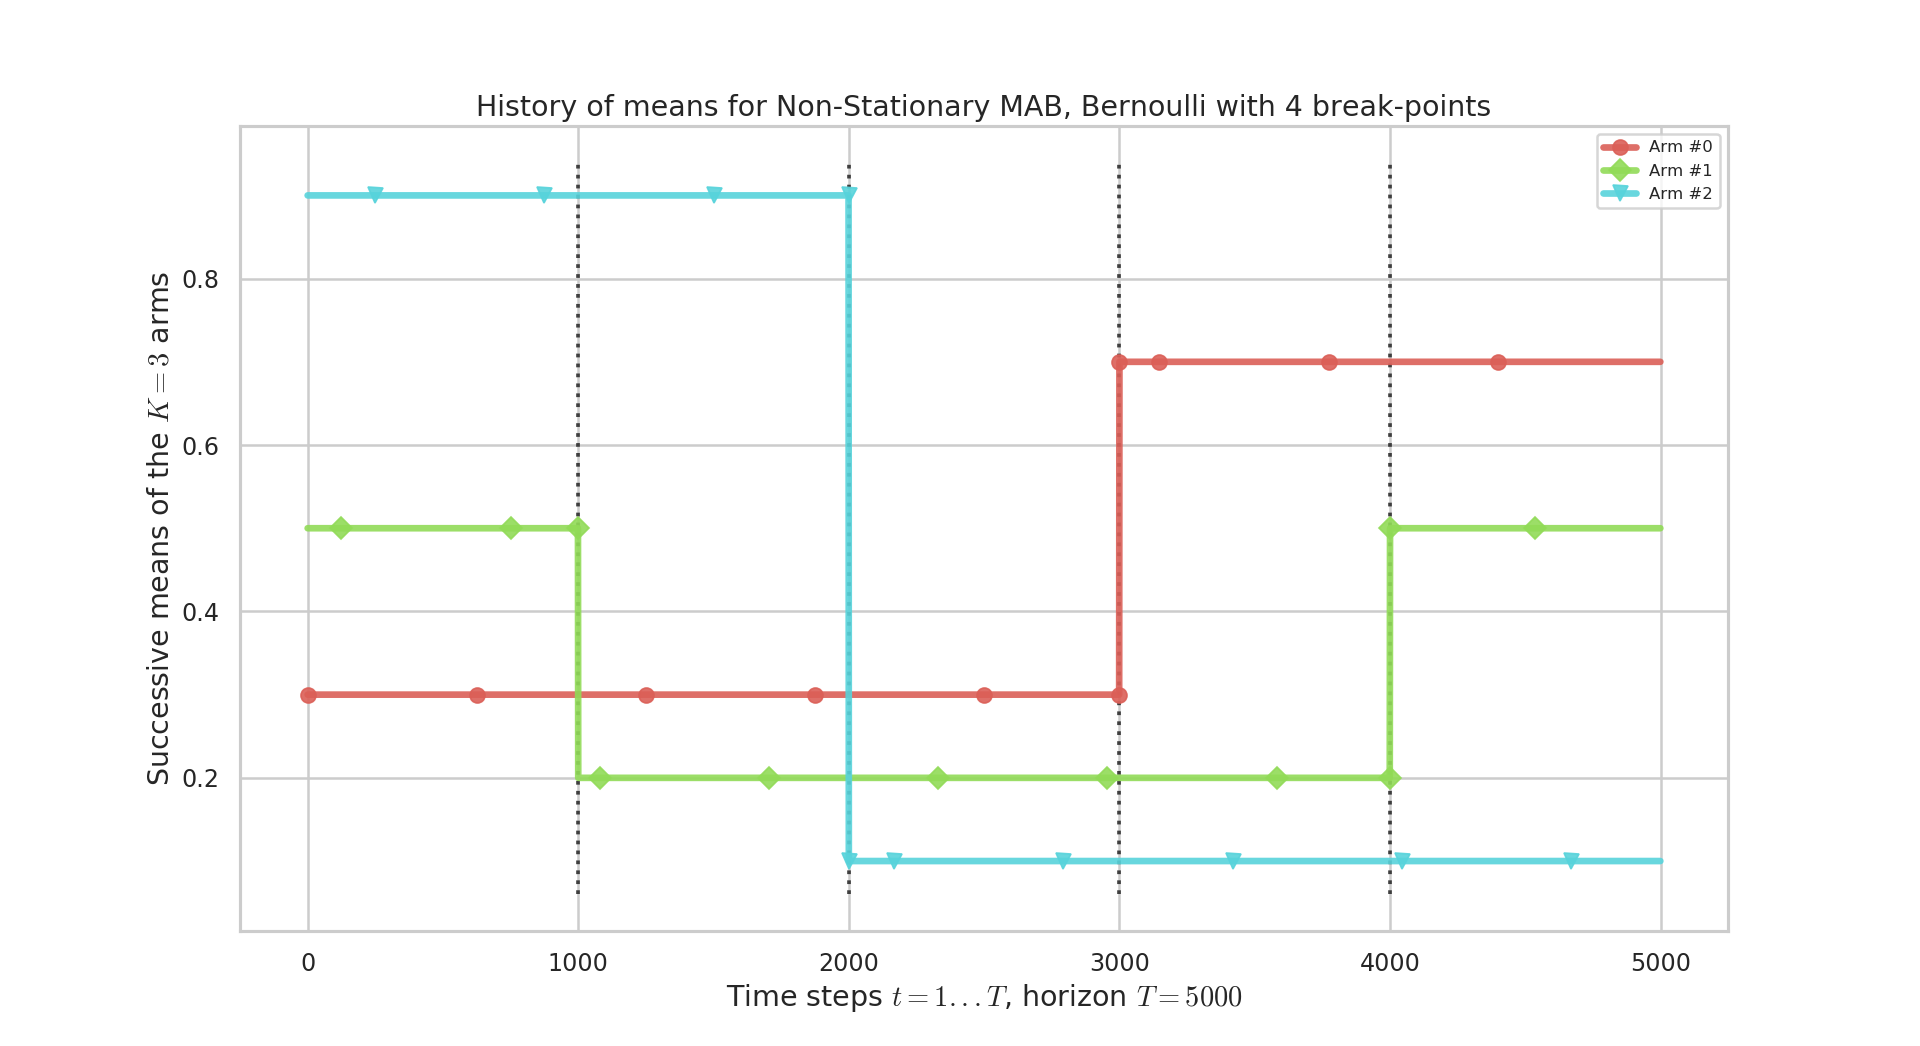
\includegraphics[width=0.90\linewidth]{2-Chapters/6-Chapter/nonstatbandits.git/figures/6_Problems/Problem_1.pdf}
    \subcaption{\textbf{Problem $1$}: $K=3$ arms with $T=5000$, and $\Upsilon=4$ changes occur on only one arm at a time (\ie, $C=4$).}
    \label{fig:6:Problem_1}
\end{figure}


% - Pb 2 changes are on all arms at a time
\textbf{Problem $\bm 2$.}
This problem is close to Problem 1, with a minimum optimality gap of $0.1$ (at any time, the smallest difference between two means is at least $0.1$),
and shown in Figure~\ref{fig:6:Problem_2}.
However, all arms change at every breakpoint (\ie, $C_T=K\Upsilon_T=12$), with identical gaps of $0.1$ for arms $0$ and $1$, and of $0.2$ for arm $2$ (between two breakpoints, the mean change of $+0.1$ for arm $0$ and $-0.1$ for arm $1$ and $-0.2$ for arm $2$).
The first optimal arm decreases at every change (\textcolor{blue}{$2$ with $\nabla$ markers}), and one arm stays the worst (\textcolor{darkgreen}{$1$ with $\diamond$ markers}).

\begin{figure}[h!]  % [htbp]
    \centering
    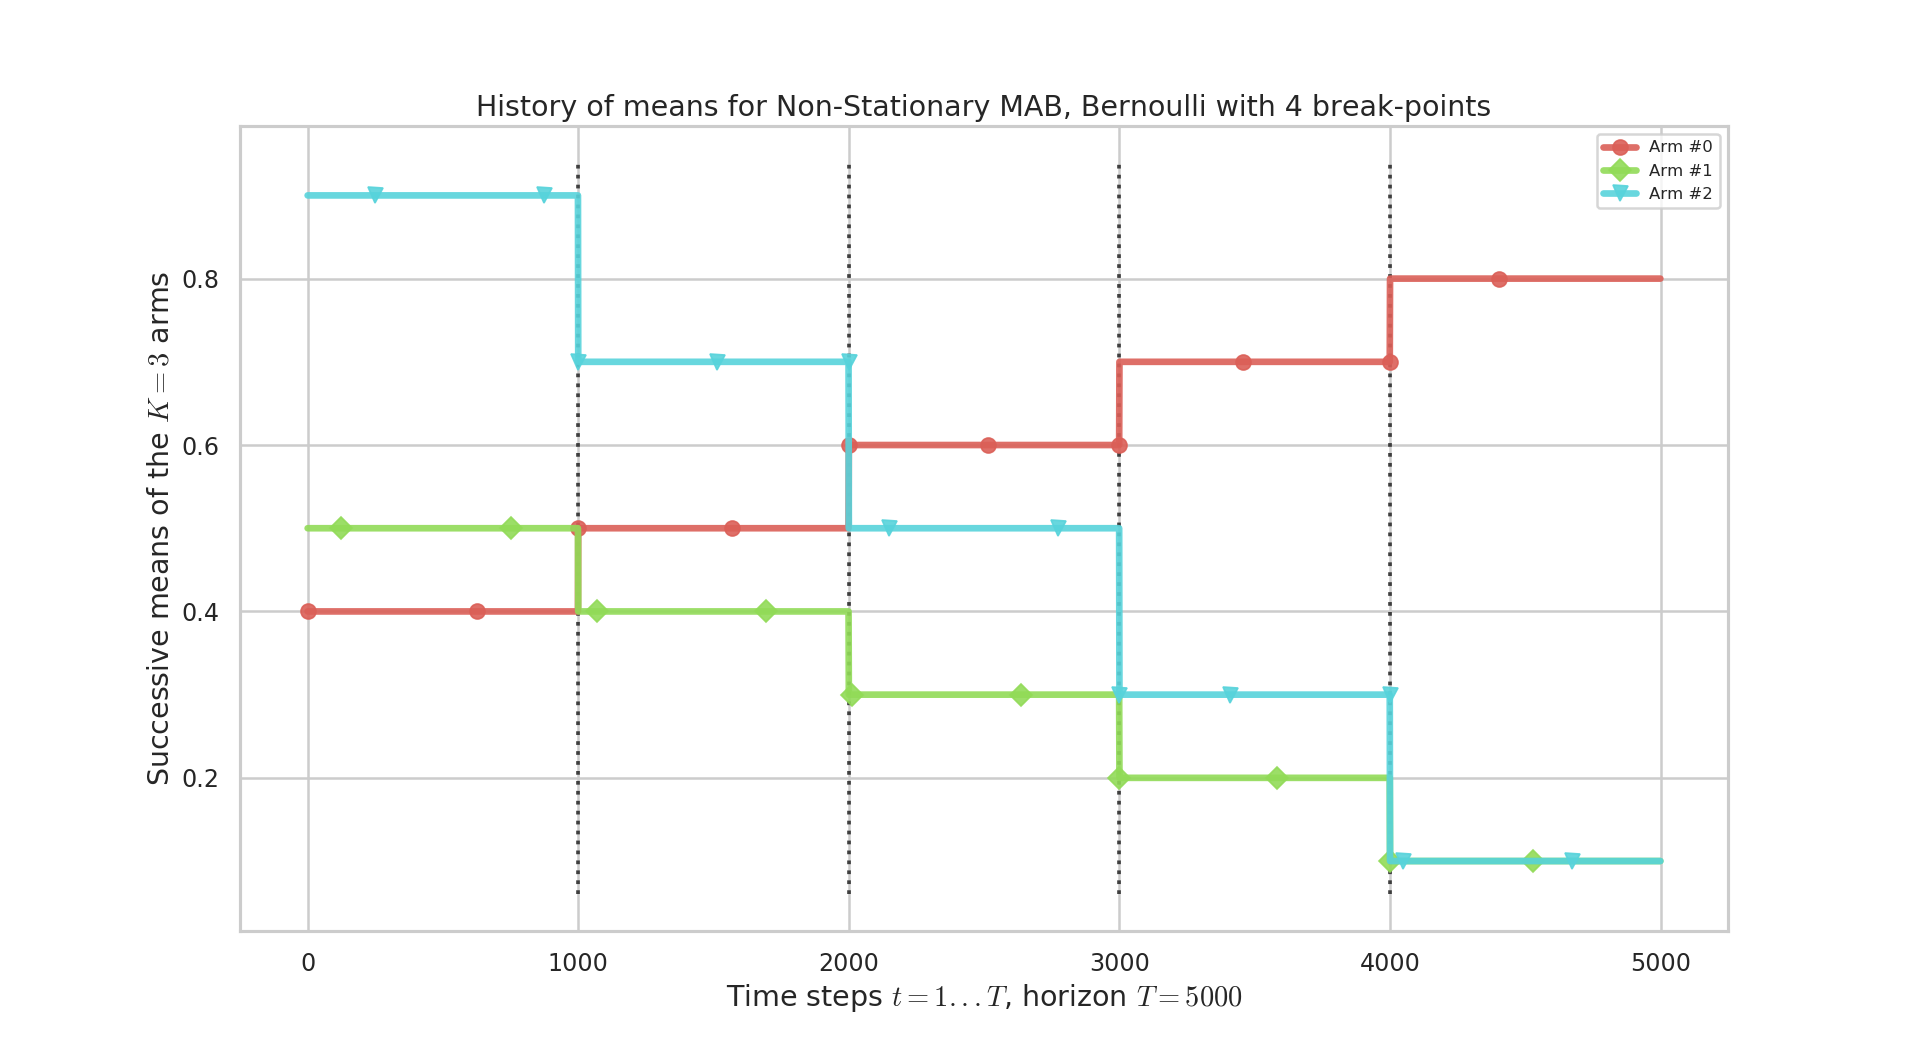
\includegraphics[width=0.90\linewidth]{2-Chapters/6-Chapter/nonstatbandits.git/figures/6_Problems/Problem_2.pdf}
    \subcaption{\textbf{Problem $2$}: $K=3$ arms with $T=5000$, and $\Upsilon=4$ changes occur on all arms (\ie, $C=12$).}
    \label{fig:6:Problem_2}
\end{figure}


% -----------------------------------------------------------
\section{Review of related works}
\label{sec:6:relatedWork}

We review previous works that studied the piece-wise stationary bandit model, or variants of this model.
To our knowledge, all the previous works are based on the idea of combining a classical bandit policy, such as Thompson sampling, \UCB{} or EXP3, with a strategy to account for changes in arms' distributions.
Following the vocabulary used in previous works, we make the distinction between passively and actively adaptive strategies.
Active strategies monitors the rewards of each arm by using a change detection algorithm \cite{Basseville93}, and reset the history of pulls and rewards of one or all the arms as soon as a change is detected.
Passive strategies use a (fixed) discount factor or a limited memory size, while most active strategies use a growing memory.
% , while active strategies are usually tuned with a threshold for the statistical test.


\paragraph{Passively adaptive algorithms.}
%
Their common idea is to adapt a classical policy into forgetting old rewards, .
If the forgetting behavior is done efficiently, then the policy can efficiently focus mostly on the most recent rewards, and passively adapt to changes when they happen.
%
The Discounted UCB (D-UCB) algorithm was first introduced in \cite{Kocsis06}, and it is an adaptation of the \UCB{} algorithm, with a discount factor $\gamma\in(0,1)$. It works by decreasing all the past rewards by a multiplicative factor, when receiving a new reward from an arm, so that the recent rewards weight more in the (discounted) empirical mean used for the computation of the \UCB{} indexes.
The regret of D-UCB was proved to be upper-bounded by $\cO(\sqrt{\Upsilon_T T }\log(T))$ in \cite{Garivier11UCBDiscount}, with a tuning $\gamma = 1 - \sqrt{\Upsilon_T/T}/4$, dependent on $\Upsilon_T$.
%
The Sliding-Window UCB (SW-UCB) uses a sliding window of a fixed size $\tau$, to store only the most $\tau$ recent rewards for each arm,
and it was proposed by \cite{Garivier11UCBDiscount}.
They prove that tuning its window-size to $\tau = 2 \sqrt{T\log(T)/\Upsilon_T}$, gives a bound on the regret of SW-UCB of the form $\cO(\sqrt{\Upsilon_T T \log(T)})$.

Both D-UCB and SW-UCB builds on a stationary policy, but for example EXP3.S from \cite{Auer02NonStochastic}
builds on the EXP3 policy, which is designed for the adversarial case.
EXP3.S actually achieves a good regret upper-bound, of the form $\cO(\sqrt{K \Upsilon_T T})$, with no additional prior knowledge except that of $T$ and $\Upsilon_T$.
It constitues a good baseline for our numerical experiments in ,
even if we did find that EXP3.S performs worse that the most of the other approaches based on extensions of stationary bandit algorithms (\eg, SW-UCB).
% , so we do not include it in .
Similarly, previous works showed that older algorithms have no or weaker regret guarantees, and have been proved to be less efficient empirically, or are designed for more specific settings.


The idea of using a simple discount factor, as for D-UCB, was recently adapted to a Bayesian policy, with the Discounted Thompson sampling (DTS) algorithm presented by \cite{RajKalyani17}.
Even if no theoretical guarantee was given, it can be empirically very efficient, but we found that DTS is not robust in the choice of if its discount factor $\gamma\in(0,1)$, contrarily to what was highlighted in the paper.
The DTS algorithm can perform well in practice, for instance with $\gamma=0.75$ on Problems $1$ and $2$ (see Section~\ref{sec:6:NumericalExperiments}). However, no theoretical guarantees are given for this strategy, and our experiments did not really confirm the robustness to $\gamma$.
%
In general, we found that passively adaptive approaches can be efficient when their parameters are well tuned, but our experiments show that actively adaptive algorithms perform significantly better.

% Finally, XXX use two discount factors at the same time, see the NEWMA algorithm from \cite{Keriven2018}.

% \TODOL{Talk about NEWMA and its possible application to generalize/improve D-UCB, \cite{Keriven2018}, if I have the time.}


\paragraph{Actively adaptive algorithms.}
%
We distinguish two families,
the first line of research uses frequentist change-point detectors \cite{Basseville93}, combined with stationary policies, usually index policies like \UCB.
When using an efficient CD algorithm with an efficient index policy, these approaches usually perform more efficiently than the passively algorithms.
%
The Adapt-EVE algorithm from \cite{Hartland06} uses a Page-Hikley (PH) Test and the \UCB{} policy, but no theoretical guarantee was given.
%
The Windowed-Mean Shift algorithm from \cite{YuMannor09} is more generic and combines any efficient bandit policy with a CD test based on a sliding window, but there approach is not applicable to the bandit setting of interest in this chapter, as they consider side observations.
%
The EXP3.R algorithm from \cite{Allesiardo15,Allesiardo17} combines a CD algorithm with EXP3, and the history of all arms are reset as soon as a suboptimal arm is detecting to become optimal.
A regret bound of $\cO(\Upsilon_T \sqrt{T \log(T)})$ was proved, even when $\Upsilon_T$ is known.

Two recent and related works use
the two-sided \CUSUM{} CD algorithm for \CUSUMUCB{} in \cite{LiuLeeShroff17}
or a specific and simpler CD algorithm for the Monitored UCB (\MUCB) algorithm introduced in \cite{CaoZhenKvetonXie18}.
%
The \CUSUM{} test is rather complicated and parametric: it uses the first $M$ samples (for a fixed $M$) from one arm to compute an average $\hat{u_0}$, and then builds two random walks, using the remaining observations for this arm. A change is detected when either random walks cross a threshold $h$.
It requires the tuning of three parameters, $M$ and $h$ as well as a drift correction parameter $\varepsilon\in(0,1)$.
The PH test, also studied in \cite{LiuLeeShroff17}, is similarly complex,
and we found that \PHT-\UCB{} perform very similarly to \CUSUMUCB{} in our experiments.
Even if it has the advantage of not requiring a parameter $M$,
it has no theoretical guarantee, so we do not include \PHT-\UCB{} in the experiments presented below.
%
In comparison, \MUCB{} uses a much simpler test, based on the $w$ most recent observations on one arm (for a fixed and even number $w$), and compares with a fixed threshold $h$ the difference of the sum of rewards for the first half and the second half. It is numerically much simpler, and has the advantage of using only a bounded memory (of the order $\bigO{K w}$ for $K$ arms).
%
Both approaches also introduced a mechanism to force a uniform exploration of each arm, parametered by $\alpha\in(0,1)$.
% \CUSUMUCB{} uses a randomized exploration, by sampling arm $i$ with probability $\alpha/K$ at each time step,
% and \MUCB{} uses a more deterministic scheme, to force exploring the $K$ arms (when the time since the last restart, $t - \tau$, is found to be in $\{1,\dots,K\}$ modulo $\left\lceil 1/\alpha \right\rceil$).
% Both solutions ensure that all arms are sampled enough on each stationary sequence, in order for the CD algorithm to have enough \iid{} samples to detect changes.

When all their parameters are tuned correctly, both approaches are proved to achieve a good regret upper-bound, of order $\cO(K \sqrt{\Upsilon_T T \log(K T)})$.
As both results are valid under different assumptions, we consider the two results to be the current state-of-the-art.
As for previous works, tuning their parameters requires to know both the horizon $T$ and the number of breakpoints $\Upsilon_T$, but most importantly it requires a prior knowledge of the problem difficulty, by assuming to know a lower bound on both the length of stationary segments (\eg, $L$ for \MUCB) and on the changes on the means of arms (\eg, $\varepsilon$ for \CUSUM).
%
\CUSUMUCB{} achieves a better regret upper bound, of the order of $\cO(\sqrt{\Upsilon_T T \log(T / \Upsilon_T)})$, but \emph{only} for Bernoulli distributions,
and when its $4$ parameters ($\alpha,\varepsilon,M,h$) are tuned based on problem-dependent knowledge.
%
\MUCB{} achieves a regret bounded by $\cO(\sqrt{\Upsilon_T T \log(T)})$, for bounded distributions, and when its $4$ parameters ($\alpha,w,b,\gamma$) are also tuned based on a problem-dependent knowledge of $\tilde{\delta}$ and $L$ (see Assumption~1 and Remark~1 in \cite{CaoZhenKvetonXie18}).


% \CUSUMUCB{} is based on a rather complicated two-sided \CUSUM{} test, that uses the first $M$ samples from one arm to compute an initial average, and then detects whether a drift of size larger than $\varepsilon$ occurred from this value by checking whether a random walk based on the remaining observations crosses a threshold $h$. Thus it requires the tuning of three parameters, $M$, $\varepsilon$ and $h$.
On the one hand, \CUSUMUCB{} performs \emph{local restarts} using this test, to reset the history of \emph{one arm} for which the test detects a change.
% \MUCB{} uses a much simpler test, based on the $w$ most recent observations from an arm: a change is detected if the absolute difference between the empirical means of the first and second halves of those $w$ observations exceeds a threshold $h$. So it requires the tuning of two parameters, $w$ and $h$.
On the other hand, \MUCB{} performs \emph{global restarts} using this test, to reset the history of \emph{all arms} whenever the test detects a change on one of the arms.
Compared to \CUSUMUCB{}, note that \MUCB{} is numerically much simpler as it only uses a bounded memory, of order $\bigO{K w}$ for $K$ arms.


\paragraph{Expert aggregation.}
%
Another of research on actively adaptive algorithms uses a Bayesian point of view.
A Bayesian CD algorithm is combined with Thompson Sampling in \cite{MellorShapiro13},
and more recently \cite{Alami17} introduced the Memory Bandit algorithm.
It is presented as efficient empirically, but no theoretical guarantee are given for these two works, and due to its complexity, we do not include it in our experiments.
The idea behind Memory Bandit is to use an expert aggregation algorithm, like EXP4 from \cite{Auer02}, modified to efficiently aggregate an growing number of experts from techniques presented in \cite{Mourtada17}.
At each time step, a new expert is introduced, and experts corresponds to different Thompson sampling algorithms, each using a different history of pulls and rewards. Intuitively, after a change-point the newest experts will soon become the most efficient, as they are learning by using rewards drawn from the new distribution(s).
%
Note that the regret bound for these methods are still open-problems,
and they are computationally more costly,
therefore we choose to not include them in our experiments.


\paragraph{Slowly-varying model.}

A different setting where the quantity of interest is not $\Upsilon_T$ but the total variational budget $V_T$, was introduced by \cite{Besbes14stochastic}, for which they proposed the RExp3 algorithm.
The total variation budget $V_T$ is defined as $\sum_{t=1}^{T-1} \sum_{i=1}^K D(\nu_i(t), \nu_i(t+1))$, for a certain measure of difference $D$, which measures how much the two distributions of any arm $i$ have changed from time $t$ to time $t+1$.
Two examples can be the total variation distance $\|\cdot\|_{TV}$ or the Kullback-Leibler divergence.
%
The RExp3 algorithm can also be qualified as passively adaptive: it is based on (non-adaptive) restarts of the EXP3 algorithm. Note that this algorithm is introduced for a different setting, where the quantity of interest is not $\Upsilon_T$ but a quantity $V_T$ called the total variational budget (satisfying $\Delta^{\text{change}} \Upsilon_T \leq V_T \leq \Upsilon_T$ with $\Delta^{\text{change}}$ the minimum magnitude of a change-point).
A regret bound of the order of $\cO(V_T^{1/3} T^{2/3})$ is proved, which is weaker than existing results in our setting.

Three recent works proposed algorithms that achieve a small regret under the two models.
For simple bandits, \cite{WeiSrivastava18Abruptly} proposed the SW-UCB\# and LM-DSEE algorithms FIXME.
For contextual bandits, \cite{Luo18} and \cite{ChenLeeLuoWei2019} FIXME.
\TODOL{Parler de ces travaux là, qui sont très forts mais pas non plus encore parfaits.}

This setting is quite different from the setting we are interested by in this chapter, and even if the most recent works on slowly-varying MAB models are very interesting, we preferred to focus on the piece-wise stationary (or abruptly changing) model,
hence we do no include any of these algorithms in the experiments presented in Section~\ref{sec:6:NumericalExperiments}.


\paragraph{Another point-of-view on prior knowledge of $\Upsilon_T$.}
%
In this chapter, like in our two main inspirational works \cite{CaoZhenKvetonXie18,LiuLeeShroff17},
we assume that the algorithm know in advance the number of break-points $\Upsilon_T$.
Another interesting point-of-view is the one presented by \cite{WeiSrivastava18Abruptly,WeiSrivastava18Distributed},
where the authors assume that there exists a number $\nu\in(0,1)$ for which $\Upsilon_T = \smallO{T^{\nu}}$,
and they also assume that any algorithm tackling such problems can know in advance the value of $\nu$ (or an upper-bound on $\nu$), and tweak its parameters from this value $\nu$, but cannot know the exact value of $\Upsilon_T$.
%
This interpretation is interesting too, but due to time and space constraints, we preferred to not explore it further.
Empirically, we found that the SW-UCB\# algorithm proposed in \cite{WeiSrivastava18Abruptly} performs comparably to SW-UCB, and thus we did not include it in the experiments presented below in Section~\ref{sec:6:NumericalExperiments}.

% \TODOL{Speak about the article \cite{WeiSrivastava18Abruptly,WeiSrivastava18Distributed} and their point of view on $\Upsilon_T = \bigO{T^{\nu}}$ with known $\nu$ but unknown $\Upsilon_T$}


\paragraph{Positionning of our results.}
%
\CUSUMUCB{} and \MUCB{} are both analyzed under some reasonable assumptions on the problem parameters --the means $(\mu_i(t))$-- mostly saying that the breakpoints are sufficiently far away from each other.
%
However, the proposed guarantees only hold for parameters \emph{tuned using some prior knowledge of the means}.
Indeed, while in both cases the threshold $h$ can be set as a function of the horizon $T$ and the number of breakpoints  $\Upsilon_T$ (also needed by previous approaches to obtain the best possible bounds), the parameter $\varepsilon$ for \CUSUM{} and $w$ for \MUCB{} require the knowledge of $\Delta^{\text{change}}$ the smallest magnitude of a change-point.
%
In this chapter, we propose \emph{the first algorithm that does not require this knowledge}, and still attains a $\cO(\sqrt{\Upsilon_T T\log(T)})$ regret.
Moreover we propose the first comparison of the use of local and global restarts within an adaptive algorithm, by studying two variants of our algorithm.
% This study is supported by both theoretical and empirical results presented in this chapter.
%
In others words, if we want to apply our proposal to piece-wise stationary problems such as problem $1$ or $2$ presented above (see Figures~\ref{fig:6:Problem_1}, \ref{fig:6:Problem_2}),
it only needs to know before hand that $T=5000$ and $\Upsilon_T=4$ for these examples, but it does not need to know the amplitude of changes $\max_{i,t} |\mu_i(t) - \mu_i(t+1)|$ nor the optimality gap or a bound on the optimality gap at any time step $\max_{i,j} |\mu_i(t) - \mu_j(t)|$.

Moreover, we can use the two problems $1$ and $2$ to illustrate the expected empirical behavior of our proposal \GLRklUCB.
Problem $1$ has only \emph{local changes}, meaning that at any change-point, only one arm sees its distribution change, while problem $2$ has only \emph{global changes}, meaning that all arms see their distribution change at each change-point.
They illustrate both the extreme cases of having $C_T = \Upsilon_T$ (for problem $1$) and $C_T = K \Upsilon_T$ (for problem $2$).
\begin{itemize}
    \item
On the one hand, we expect the \emph{local restart} variant of \GLRklUCB{} to outperform the \emph{global restart} variant for problem $1$, as the intuition suggests that it is sub-optimal to reinitialize the memory of the observations of the $K-1$ arms whose distributions did not change after a change-point is detected (as the \emph{global restart} variant do).
    \item
On the other hand, we expect the \emph{global restart} variant to outperform the \emph{local restart} variant for problem $2$, as detecting a change one any arm is enough to know that all arms changed and to reinitialize the memory of all arms, and thus the intuition suggests that it is sub-optimal to reinitialize only the memory of the observation of the arm on which the change-point was detected (as the \emph{local restart} variant do).
\end{itemize}
%
Of course, on a given problem, without additional prior knowledge on the difficulty of the problem at hand, the algorithm cannot know which situation is more likely to happen, only local changes ($C_T = \Upsilon_T$) or only global changes ($C_T = K \Upsilon_T$) or any intermediate setting between the two extreme cases.
Thus we do not believe to be able to design a policy that could be uniformly better than the two variants of \GLRklUCB.
%
Surprisingly, numerical experiments show that the \emph{local} variant of \GLRklUCB{} actually outperforms the \emph{glocal} variant for both problem $1$ and $2$, as shown below in Table~\ref{table:6:totalResults1}, and in other problems as shown in Table~\ref{table:6:totalResults2}.
%
Understanding this difference in terms of numerical performance of the two variants is left as future work.

Finally, on the practical side, while we can note that the proposed B-GLRT test is more complex to implement than the test used by \MUCB, we propose two heuristics to speed it up while not losing much in terms of regret, in Appendix~\ref{sub:6:IdeasOptimizations}.


\paragraph{About \klUCB.}
%
Our proposal \GLRklUCB{} is inspired by both the \MUCB{} and \CUSUMUCB{} algorithms.
Previous works focussed on using \UCB{} \cite{LiuLeeShroff17,CaoZhenKvetonXie18},
but we propose to use \klUCB{} instead, as it is known to be more efficient for Bernoulli rewards as well as for a more generic case of bounded or one-dimensional exponential families \cite{KLUCBJournal}.
Theoretical results for these works were only given for \UCB, but they both suggest that extending the results to \klUCB{} (or other efficient stationary policies) should not be difficult.
For a fair comparison, we therefore chose to compare the different change-point detector algorithms combined with \klUCB.


% -----------------------------------------------------------------
\section{The Bernoulli GLRT Change-Point Detector}
\label{sec:6:ChangePointDetector}

Sequential change-point detection has been extensively studied in the statistical community.
We refer to the book \cite{Basseville93} for a survey.
%
In this section, we are interested in detecting changes on the mean of a probability distribution with bounded support.

Assume that we collect independent samples $X_1,X_2,\ldots$ all from some distribution supported in $[0,1]$.
We want to discriminate between two possible scenarios: all the samples come from distributions that have a common mean $\mu_0$, or there exists a \emph{change-point} $\tau > 1$ such that $X_1,\ldots,X_\tau$ have some mean $\mu_0$ and $X_{\tau +1},X_{\tau+2},\ldots$ have a different mean $\mu_1 \neq \mu_0$.
%
A sequential change-point detector is a stopping time $\widehat{\tau}$ with respect to the filtration $\cF_t = \sigma(X_1,\dots,X_t)$ such that $(\hat \tau < \infty)$ means that we reject the hypothesis
$\cH_0 : \left(\exists \mu_0 \in [0,1]: \forall i\in\N^*, \bE[X_i] = \mu_0\right)$.

Generalized Likelihood Ratio tests date back to the seminal work of \cite{Wilks1938}, and were for instance studied for change-point detection by \cite{barnard1959control,siegmund1995using}.
Exploiting the fact that bounded distribution are $(1/4)$-sub Gaussian (\ie, their moment generating function is dominated by that of a Gaussian distribution with the same mean and a variance $1/4$), the (Gaussian) GLRT, recently studied in depth by \cite{Maillard2018GLR}, can be used for this problem.
We propose instead to exploit the fact that bounded distributions are also dominated by Bernoulli distributions.

\begin{definition}[Sub-Bernoulli distributions]
    We call a \emph{sub-Bernoulli distribution} any distribution $\nu$ that satisfies
    $\ln \bE_{X\sim\nu}\left[e^{\lambda X}\right] \leq \phi_{\mu}(\lambda)$ with $\mu=\bE_{X\sim \nu}[X]$ and $\phi_{\mu}(\lambda) = \ln(1-\mu + \mu e^\lambda)$ is the log moment generating function of a Bernoulli distribution with mean $\mu$, for any $\mu\in[0,1]$.
\end{definition}

Lemma~1 of \cite{KLUCBJournal} establishes that any bounded distribution supported in $[0,1]$ is a sub-Bernoulli distribution.
Our work can be applied to any bounded distribution without loss of generality, as a reward in $r\in[a,b]$ can clearly be mapped to $[0,1]$ simply by using $r' = (r-a)/(b-a)$ (we assume that the decision maker or the algorithm know before hand the values of $a,b$).


\subsection{Presentation of the test}\label{sub:6:presentationOfGLRTest}

If the samples $(X_t)$ were all drawn from a Bernoulli distribution, this change-point detection problem introduced above would reduce to a parametric sequential test of
\[\cH_0 : (\exists \mu_0: \forall i\in\N, X_i \ \overset{\text{i.i.d.}}{\sim} \ \cB(\mu_0)),\]
against the alternative
\[\cH_1 : (\exists \mu_0 \neq \mu_1, \tau \in \N^*: \ \  X_1, \ldots, X_\tau \ \overset{\text{i.i.d.}}{\sim} \ \cB(\mu_0) \ \ \text{and} \ \ X_{\tau+1}, X_{\tau+2}, \ldots \ \overset{\text{i.i.d.}}{\sim} \ \cB(\mu_1)).\]

The Generalized Likelihood Ratio statistic for this test is defined by
\begin{equation}\label{eq:6:firstDefGLRT}
    \GLR(n) :=\frac{\sup\limits_{\mu_0,\mu_1,\tau < n}\ell(X_1, \ldots, X_n ; \mu_0,\mu_1,\tau)}{\sup\limits_{\mu_0}\ell(X_1, \ldots, X_n ; \mu_0)},
\end{equation}
%
where $\ell(X_1, \ldots, X_n ; \mu_0)$ and $\ell(X_1, \ldots, X_n ; \mu_0,\mu_1,\tau)$ respectively denote the \emph{likelihoods} of the first $n$ observations under a model in $\cH_0$ and $\cH_1$.
High values of this statistic tend to indicate rejection of $\cH_0$.
%
By using the form of the likelihood for Bernoulli distributions, this statistic can be written with the binary relative entropy $\kl$, defined for $x,y\in[0,1]$ (with the usual convention that $t \log(t) = 0$ if $t=0$).
%
\begin{equation}\label{eq:6:BernoulliDivergence}
    \kl(x,y) := x \ln\left(\frac{x}{y}\right) + (1-x)\ln\left(\frac{1-x}{1-y}\right).
\end{equation}
%
Indeed, we show below
% in Appendix~\ref{app:6:GLR_with_kl}
that in any one-dimensional exponential family, we have
\begin{equation}\label{eq:6:secondDefGLRT}
    \log \GLR(n) = \sup_{s \in [2,n-1]} \left[s \times \kl\left(\widehat{\mu}_{1:s},\widehat{\mu}_{1:n}\right) + (n-s) \times \kl\left(\widehat{\mu}_{s+1:n},\widehat{\mu}_{1:n}\right)\right].
\end{equation}
%
where for $k \leq k'$, $\widehat{\mu}_{k:k'} := \frac{1}{k - k' + 1} \sum_{l=k}^{k'} X_l$ denotes the average of the observations $X_l$ collected between the instants $k$ and $k'$.


\begin{proof}
    First, we consider the denominator in the expression of $\GLR(n)$ \eqref{eq:6:firstDefGLRT}, that is the $\sup$ on $\mu_0$.
    We have $\ell(X_1, \ldots, X_n ; \mu_0) = \prod_{i=1}^n \ell(X_i ; \mu_0)$ by independence of the observations $X_i$,
    and $\ell(X_i ; \mu_0) = \mu_0^{X_i} (1-\mu_0)^{1-X_i}$ for Bernoulli distributions.
    Therefore, taking the logarithm gives
    \begin{align*}
        \log\ell(X_1, \ldots, X_n ; \mu_0)
        &= \sum_{i=1}^n X_i \log(\mu_0) + (1-X_i) \log(1-\mu_0) \\
        &= \log(\mu_0) \times \left( \sum_{i=1}^n X_i \right) + \log(1-\mu_0) \times \left( n - \sum_{i=1}^n X_i \right) \\
        &= n \left[ \widehat{\mu}_{1:n} \log(\mu_0) + (1 - \widehat{\mu}_{1:n}) \log(1-\mu_0) \right].
    \end{align*}
    %
    For a constant $a\in[0,1]$, let $h(x) := a \log(x) + (1-a) \log(1-x)$ on $(0,1)$,
    and we are trying to solve $\sup_{x\in[0,1]} h(x)$.
    If $a=0$ or $a=1$, $h$ is maximum at $x=a$.
    Now if $a\neq0$, As $h$ is of class $\cC^1$, we can just differentiate and find the root of its derivative:
    $h'(x) = a/x - (1-a)/(1-x)$, so $h'(x) = 0$ if and only if $x=a$.
    Thus in all cases, $\sup_{x\in[0,1]} h(x) = h(a)$.
    %
    Here, we have $a = \widehat{\mu}_{1:n}$, and thus we solve the $\sup_{\mu_0}$ optimization problem found in the denominator of the $\GLR(n)$ expression.
    By replacing $\mu_0 = \widehat{\mu}_{1:n}$, we obtained the following (unique) solution,
    \begin{equation}\label{eq:6:solutionPbOpt_for_1n}
        \sup_{\mu_0} \log\ell(X_1, \ldots, X_n ; \mu_0) = n \left( \widehat{\mu}_{1:n} \log(\widehat{\mu}_{1:n}) + (1 - \widehat{\mu}_{1:n}) \log(1-\widehat{\mu}_{1:n}) \right).
    \end{equation}

    Now let us consider the nominator of the $\GLR(n)$ expression.
    We can again work with log-likelihoods, and so we have
    \begin{align*}
        & \log\ell(X_1, \ldots, X_n ; \mu_0,\mu_1,\tau) \\
        &= \sum_{i=1}^{\tau} X_i \log(\mu_0) + (1-X_i) \log(1-\mu_0) + \sum_{i=\tau+1}^n X_i \log(\mu_1) + (1-X_i) \log(1-\mu_1) \\
        &= s \bigl( \widehat{\mu}_{1:s} \log(\mu_0) + (1 - \widehat{\mu}_{1:s}) \log(1-\mu_0) \bigr) \\
        & \;\;\;\; + (n-s) \bigl( \widehat{\mu}_{s+1:n} \log(\mu_1) + (1 - \widehat{\mu}_{s+1:n}) \log(1-\mu_1) \bigr).
    \end{align*}
    Because we solved in \eqref{eq:6:solutionPbOpt_for_1n} the $\sup$ for the denominator,
    we have
    \begin{align*}
        \GLR(n)
        % &= \frac{\sup\limits_{\mu_0,\mu_1,\tau < n}\ell(X_1, \ldots, X_n ; \mu_0,\mu_1,\tau)}{\sup\limits_{\mu_0}\ell(X_1, \ldots, X_n ; \mu_0)}, \\
        &= \frac{\sup\limits_{\mu_0,\mu_1,\tau < n}\ell(X_1, \ldots, X_n ; \mu_0,\mu_1,\tau)}{ \exp\left[ n \left( \widehat{\mu}_{1:n} \log(\mu_0) + (1 - \widehat{\mu}_{1:n}) \log(1-\mu_0) \right) \right] }, \\
        &= \sup\limits_{\mu_0,\mu_1,\tau < n} \frac{\ell(X_1, \ldots, X_n ; \mu_0,\mu_1,\tau)}{ \exp\left[ n \left( \widehat{\mu}_{1:n} \log(\widehat{\mu}_{1:n}) + (1 - \widehat{\mu}_{1:n}) \log(1-\widehat{\mu}_{1:n}) \right) \right] }, \\
        &= \exp \Bigl[ \sup\limits_{\mu_0,\mu_1,\tau < n} \Bigl[ \log\Bigl[ \frac{\ell(X_1, \ldots, X_n ; \mu_0,\mu_1,\tau)}{ \exp\left[ n \left( \widehat{\mu}_{1:n} \log(\widehat{\mu}_{1:n}) + (1 - \widehat{\mu}_{1:n}) \log(1-\widehat{\mu}_{1:n}) \right) \right] } \Bigr] \Bigr] \Bigr],  \\
        &= \exp \Bigl[ \sup\limits_{\mu_0,\mu_1, 1 < s < n} \Bigl[
            s \bigl( \widehat{\mu}_{1:s} \log(\mu_0) + (1 - \widehat{\mu}_{1:s}) \log(1-\mu_0) \bigr) \\
            & \hspace{35pt} + (n-s) \bigl( \widehat{\mu}_{s+1:n} \log(\mu_1) + (1 - \widehat{\mu}_{s+1:n}) \log(1-\mu_1) \bigr) \\
            & \hspace{35pt} - n \bigl( \widehat{\mu}_{1:n} \log(\widehat{\mu}_{1:n}) + (1 - \widehat{\mu}_{1:n}) \log(1-\widehat{\mu}_{1:n}) \bigr)
        \Bigr] \Bigr].
    \end{align*}
    By linearity and independence, we can separate the joint optimization problem on $\mu_0,\mu_1,s$ in two optimizations problems for $\mu_0,s$ and $\mu_1,s$, that can first be solved explicitly for $\mu_0$ (resp. $\mu_1$) and then left to be solved for $s$.
    By definition, $n \; \widehat{\mu}_{1:n} = \sum_{i=1}^n X_i = s \;\widehat{\mu}_{1:s} + (n-s) \;\widehat{\mu}_{s+1:n}$, so the right hand side (negative) part involving $\widehat{\mu}_{1:n}$ can be distributed in the two left hand side (positive) terms,
    which are both handled similarly.
    For instance for $\mu_0$, we use the same computation as above with the function $h$ to find the optimum:
    $\widehat{\mu}_{1:s} \log(\mu_0) + (1 - \widehat{\mu}_{1:s}) \log(1-\mu_0)$
    is optimum for $\mu_0 = \widehat{\mu}_{1:s}$.
    Similarly, the term for $\mu_1$ gives that $\sup_{\mu_1} \widehat{\mu}_{s+1:n} \log(\mu_1) + (1 - \widehat{\mu}_{s+1:n}) \log(1-\mu_1)$
    is attained for $\mu_1 = \widehat{\mu}_{s+1:n}$.
    Finally, by replacing the two expressions of the solutions for $\mu_0$ and $\mu_1$,
    we obtain
    \begin{align*}
        \GLR(n)
        = \exp \Bigl[ \sup\limits_{1 < s < n} \Bigl[
            s \times \Bigl(
                    & \widehat{\mu}_{1:s} \log(\widehat{\mu}_{1:s}) + (1 - \widehat{\mu}_{1:s}) \log(1-\widehat{\mu}_{1:s}) \\
                    & - \widehat{\mu}_{1:s} \log(\widehat{\mu}_{1:n}) + (1 - \widehat{\mu}_{1:s}) \log(1-\widehat{\mu}_{1:n})
            \Bigr) \\
            + (n-s) \times \Bigl(
                & \widehat{\mu}_{s+1:n} \log(\widehat{\mu}_{s+1:n}) + (1 - \widehat{\mu}_{s+1:n}) \log(1-\widehat{\mu}_{s+1:n}) \\
                & - \widehat{\mu}_{s+1:n} \log(\widehat{\mu}_{1:n}) + (1 - \widehat{\mu}_{s+1:n}) \log(1-\widehat{\mu}_{1:n})
            \Bigr)
        \Bigr] \Bigr].
    \end{align*}
    We conclude by recognizing the expressions of $s \times \kl(\widehat{\mu}_{1:s}, \widehat{\mu}_{1:n})$
    and $(n-s) \times \kl(\widehat{\mu}_{s+1:n}, \widehat{\mu}_{1:n})$.
\end{proof}


This motivates the following definition of the Bernoulli GLRT change point detector.
% Note that the $\exp$ appearing in the \eqref{eq:6:secondDefGLRT} is absorbed as a $\log$ in the threshold function $\beta$.

\begin{definition}\label{def:6:GLRDef}
    The Bernoulli GLRT (B-GLRT) change point detector with threshold function $\beta(n,\delta)$ is the stopping time $\widehat{\tau}_{\delta}$ defined by
    %
    \begin{equation}\label{def:6:GLR}
        \widehat{\tau}_{\delta} := \inf \left\{ n \in \N^* : \sup_{s \in [2,n-1]} \left[s \times \kl\left(\widehat{\mu}_{1:s},\widehat{\mu}_{1:n}\right) + (n-s) \times \kl\left(\widehat{\mu}_{s+1:n},\widehat{\mu}_{1:n}\right)\right] \geq \beta(n,\delta)\right\}.
    \end{equation}
\end{definition}

Asymptotic properties of the GLRT for change-point detection have been studied by \cite{LaiXing10} for Bernoulli distributions and more generally for one-parameter exponential families, for which the GLR test is defined as in~\eqref{def:6:GLR}, but with $\kl(x,y)$ replaced by the Kullback-Leibler divergence $d(x,y)$ between two elements in that exponential family that have mean $x$ and $y$.
For example, the Gaussian GLR studied by \cite{Maillard2018GLR} corresponds to the stopping time \eqref{def:6:GLR} with the choice $d(x,y) = 2(x-y)^2$, when the variance is set to $\sigma^2=1/4$, and non-asymptotic properties of this test are given for any $(1/4)$-subGaussian samples.
Note that Pinsker's inequality gives that $\kl(x,y) \geq 2(x-y)^2$ (see Lemma~\ref{lem:6:Pinsker}), hence the B-GLRT may stop earlier that the Gaussian GLR, based on the quadratic divergence $d(x,y) = 2(x-y)^2$.
%
In the next section, we provide new non-asymptotic results about the B-GLRT under the assumption that the samples $(X_t)$ come from a sub-Bernoulli distribution, which holds for any distribution supported in $[0,1]$.


% ----------------------------------------------------------------------------
\subsection{Non-asymptotic properties of the B-GLRT}\label{subsec:6:PropGLR}

When used for a bandit problem, the two main properties of a sequential change-point detection test are its false alarm probability and its detection delay.
%
A small false alarm probability ensures that no detection occurs before it should (\ie, no useless detection occur on stationary segments), and a small detection delay ensures that, if the stationary segments are long enough, then every change-points on every arms will be detected after a short enough amount of samples from that arm.
%
We give below two lemmas, Lemma~\ref{lem:6:FalseAlarm} which bounds the false alarm probability for a choice of threshold function, and Lemma~\ref{lem:6:Delay} which bounds the detection delay if there is enough samples before a change.


%-----------------------------------------------------------------------------
\paragraph{False alarm probability.}\label{par:6:falseAlarm}

In Lemma~\ref{lem:6:FalseAlarm} below, we propose a choice of the threshold function $\beta(n,\delta)$ under which the probability that there exists a \emph{false alarm} under \iid{} data is small. To define $\beta$, we need to introduce the function $\cT$, defined for $x>0$ by
%
\begin{equation}\label{def:6:function_T}
    \cT(x) ~:=~ 2 \widetilde{h}\left(\frac{h^{-1}(1+x) + \ln(2\zeta(2))}{2}\right),
\end{equation}
where for $u \ge 1$ we define $h(u) = u - \ln(u)$ and its inverse $h^{-1}(u)$,
%
we define $\widetilde{h}(x) = e^{1/h^{-1}(x)} h^{-1}(x)$ if $x \ge h^{-1}(1/\ln (3/2))$ and $\tilde{h}(x) = (3/2) (x-\ln(\ln (3/2)))$ otherwise, for any $x \ge 0$,
and with the value $\zeta(2) = \pi^2 / 6$.
%
Even if it does not have a closed form expression, the function $\cT$ is easy to compute numerically.
%
The inverse $h^{-1}$ can be computed using $\mathcal{W}$, the Lambert $\mathcal{W}$ function \cite{Corless96}, which is the inverse of $x \mapsto x \exp(x)$, as $h^{-1}(x) = - \mathcal{W}(- \exp(-x))$.

The use of $\cT$ for the construction of concentration inequalities that are uniform in time is detailed in~\cite{KK18Martingales}, where tight upper bound on this function $\cT$ are also given:
$\cT (x) \simeq x + 4 \ln\big(1 + x + \sqrt{2x}\big)$ for $x\geq 5$ and $\cT(x) \sim x$ when $x$ is large.

\begin{lemma}\label{lem:6:FalseAlarm}
    Let be $\bP_{\mu_0}$ a probabilistic model under which $X_t \in [0,1]$, and $X_t$ has an average of $\mu_0$ for all $t$.
    % Assume that there exists $\mu_0 \in [0,1]$ such that $\bE[X_t] = \mu_0$ and that $X_i \in [0,1]$ for all $i$.
    Then the B-GLRT test given in Definition~\ref{def:6:GLRDef} satisfies
    $\bP_{\mu_0}(\widehat{\tau}_\delta < \infty) \leq \delta$, with the threshold function
    %
    \begin{equation}\label{def:6:beta}
        \beta(n,\delta) = 2\cT\left(\frac{\ln(3n\sqrt{n}/\delta)}{2}\right) + 6\ln(1+\ln(n)).
    \end{equation}
\end{lemma}

\begin{proof}
Lemma~\ref{lem:6:FalseAlarm} is presented for bounded distributions and is actually valid for any sub-Bernoulli distribution. It could also be presented for more general distributions satisfying
\begin{equation}
    \bE[e^{\lambda X} ] \leq e^{\phi_\mu(\lambda)} \ \ \text{ with } \ \ \mu=\bE[X]\label{def:6:subExpo},
\end{equation}
where $\phi_\mu(\lambda)$ is the $\mathrm{log}$ moment generating of some one-dimensional exponential family. The Bernoulli divergence $\kl(x,y)$ would be replaced by the corresponding divergence in that exponential family (which is the Kullback-Leibler divergence between two distributions of means $x$ and $y$).

Let us go back to the Bernoulli case with divergence given in \eqref{eq:6:BernoulliDivergence}.
We first observe that
\[s \times \kl\left(\widehat{\mu}_{1:s},\widehat{\mu}_{1:n}\right) + (n-s) \times \kl\left(\widehat{\mu}_{s+1:n},\widehat{\mu}_{1:n}\right) = \inf_{\lambda \in [0,1]}\left[s \times \kl\left(\widehat{\mu}_{1:s},\lambda\right) + (n-s) \times \kl\left(\widehat{\mu}_{s+1:n},\lambda\right)\right].\]
Hence the probability of a false alarm occurring is upper bounded as
%
\begin{align*}
    \bP_{\mu_0}\left(T_{\delta} < \infty\right) & \leq \bP_{\mu_0}\left(\exists (s,n) \in \N^2, s < n:  s \, \kl\left(\widehat{\mu}_{1:s},\widehat{\mu}_{1:n}\right) + (n-s) \, \kl\left(\widehat{\mu}_{s+1:n},\widehat{\mu}_{1:n}\right) > \beta(n,\delta)\right)\\
    & \leq \bP_{\mu_0}\left(\exists (s,n) \in \N^2, s < n:  s \, \kl\left(\widehat{\mu}_{1:s},\mu_0\right) + (n-s) \, \kl\left(\widehat{\mu}_{s+1:n},\mu_0\right) > \beta(n,\delta)\right) \\
% \end{align*}%FIXME uncomment this if needed
% \begin{align*}
    & \leq \sum_{s =1}^{\infty} \bP_{\mu_0}\left(\exists n > s:  s \, \kl\left(\widehat{\mu}_{1:s},\mu_0\right) + (n-s) \, \kl\left(\widehat{\mu}_{s+1:n},\mu_0\right) > \beta(n,\delta)\right)\\
    & =   \sum_{s =1}^{\infty} \bP_{\mu_0}\left(\exists r \in \N^*:  s \, \kl\left(\widehat{\mu}_{s},\mu_0\right) + r \, \kl\left(\widehat{\mu}'_{r},\mu_0\right) > \beta(s+r,\delta)\right),
\end{align*}
%
where $\widehat{\mu}_{s}$ and $\widehat{\mu}'_{r}$ are the empirical means of respectively $s$ and $r$ \iid{} observations with mean $\mu_0$ and distribution $\nu$, that are independent from the previous ones.
As $\nu$ is sub-Bernoulli, the conclusion follows from Lemma~\ref{lem:6:ConcFirst} below and from the definition of $\beta(n,\delta)$, if we denote $F(x)=\ln(1+\ln(x))$,
%
\begin{align*}
    &\bP_{\mu_0}\left(T_{\delta} < \infty\right) \\
    & \leq \sum_{s =1}^{\infty} \bP_{\mu_0}\left(\exists r \in \N^* : s \, \kl\left(\widehat{\mu}_{s},\mu_0\right) + r \, \kl\left(\widehat{\mu}'_{r},\mu_0\right) > 6F(s+r)+ 2 \cT\left(\frac{\ln(3(s+r)^{3/2}/\delta)}{2}\right)\right)\\
    & \leq \sum_{s =1}^{\infty} \bP_{\mu_0}\left(\exists r \in \N^* : s \, \kl\left(\widehat{\mu}_{s},\mu_0\right) + r \, \kl\left(\widehat{\mu}'_{r},\mu_0\right) > 3F(s)+3F(r) + 2 \cT\left(\frac{\ln(3s^{3/2}/\delta)}{2}\right)\right)
\end{align*}
%
And so we have $\bP_{\mu_0}\left(T_{\delta} < \infty\right) \leq \sum_{s =1}^{\infty} \frac{\delta}{3s^{3/2}} \leq \delta$.
%
\end{proof}

\begin{lemma}\label{lem:6:ConcFirst}
    $(X_i)_{i \in \N^*}$ and $(Y_i)_{i \in \N^*}$ two independent \iid{} processes with respective means $\mu$ and $\mu'$ such that
    $\bE[e^{\lambda X_1}] \leq e^{\phi_{\mu}(\lambda)}$ and $\bE[e^{\lambda Y_1}] \leq e^{\phi_{\mu'}(\lambda)}$,
    where $\phi_\mu(\lambda) = \bE_{X \sim \nu^{\mu}}[e^{\lambda X}]$ is the moment generating function of the distribution $\nu^\mu$, which is the unique distribution in an exponential family that has mean $\mu$.

    Let $\kl(\mu,\mu') = \KL(\nu^\mu,\nu^{\mu'})$ be the divergence function associated to that exponential family. Introducing the notation $\widehat{\mu}_s = \frac{1}{s}\sum\limits_{i=1}^s X_i$ and $\widehat{\mu}'_r = \frac{1}{r}\sum\limits_{i=1}^r Y_i$, it holds that for every $s,r \in \N^*$,
    \[\bP\left(\exists r \in \N^* : s \, \kl\left(\widehat{\mu}_{s},\mu\right) + r \, \kl\left(\widehat{\mu}_r',\mu'\right) > 3\ln(1+\ln(s)) + 3\ln(1+\ln(r)) + 2\cT\left(\frac{x}{2}\right)\right)\leq e^{-x},\]
    where $\cT$ is the function defined in \eqref{def:6:function_T}.
\end{lemma}
\begin{proof}
    This Lemma~\ref{lem:6:ConcFirst} is proved in Appendix~\ref{app:6:proofConcFirst}.
\end{proof}


%-----------------------------------------------------------------------------
\paragraph{Detection delay.}

Another key feature of a change-point detector is its \emph{detection delay} under a model in which a change from $\mu_0$ to $\mu_1$ occurs at time $\tau$. We already observed that from Pinsker's inequality (Lemma~\ref{lem:6:Pinsker}), the B-GLRT stops earlier than a Gaussian GLR. Hence, one can leverage some techniques from \cite{Maillard2018GLR} to upper bound the detection delay of the B-GLRT. Letting $\Delta = |\mu_0 - \mu_1|$, one can essentially establish that for $\tau$ larger than $(1/\Delta^2)\ln(1/\delta)$ (\ie, enough samples before the change), the delay can be of the same magnitude (\ie, enough samples after the change).
In the bandit analysis to follow, the detection delay will be crucially used to control the probability of the good event (in Lemma~\ref{lem:6:GoodEventGlobal} and \ref{lem:6:GoodEvent}).

\begin{lemma}\label{lem:6:Delay}
    Let be $\bP_{\mu_0,\mu_1,\tau}$ a probabilistic model under which $X_t \in [0,1]$, and $X_t$ has an average of $\mu_0$ for all $t \leq \tau$, and $\mu_1$ for all $t > \tau$, with $\mu_0 \neq \mu_1$,
    and let $\Delta = |\mu_0 - \mu_1|$.
    Then the B-GLRT test given in Definition~\ref{def:6:GLRDef} satisfies
    \begin{equation}
        \bP_{\mu_0,\mu_1,\tau} (\widehat{\tau}_{\delta} \geq \tau + u) \leq \exp\left( -\frac{2\tau u}{\tau + u}\left(\max\left[ 0, \Delta - \sqrt{\frac{\tau + u}{2\tau u} \beta(\tau + u,\delta)} \right]\right)^2 \right).
    \end{equation}
\end{lemma}
%
\begin{proof}
    It is actually not used as such in the proofs of the regret upper bound given below, but a similar result is used and proved in the proofs.
    \TODOL{We have to give the proof, or remove this result!}
\end{proof}

For a threshold $\beta$ chosen as in the Lemma~\ref{lem:6:FalseAlarm}, we can show that a consequence of the Lemma~\ref{lem:6:Delay} is that if the break-point $\tau$ takes place after $\Delta^{-2} \ln(1/\delta)$ samples, the detection time may be of the same magnitude (with high probability).
%
In other words, if the B-GLRT test observes enough samples before a change-point,
its delay $\widehat{\tau}_\delta$ is in the order of $O(\Delta^{-2} \ln(1/\delta))$, with high probability.


% ----------------------------------------------------------------------------
\subsection{Practical considerations}\label{sub:6:PracticalConsiderations}

Lemma~\ref{lem:6:FalseAlarm} provides the first non-asymptotic control of false alarm for the B-GLRT employed for bounded data. However, the threshold \eqref{def:6:beta} is not fully explicit as the function $\cT(x)$ can only be computed numerically.
Note that for sub-Gaussian distributions, results from \cite{Maillard2018GLR} show that the smaller and more explicit threshold
$\beta(n,\delta) = \left(1 + \frac{1}{n}\right)\ln\left(\frac{3n\sqrt{n}}{\delta}\right)$,
can be used to prove an upper bound of $\delta$ for the false alarm probability of the GLR, with quadratic divergence $\kl(x,y)=2(x-y)^2$.
%
For the B-GLRT, numerical simulations suggest that the threshold \eqref{def:6:beta} is a bit conservative (see Appendix~\ref{sec:6:exploringDifferentThresholdFunctions}), and in practice we recommend to keep only the leading term and use $\beta(n,\delta) = \ln(3n^{3/2}/\delta) = \ln(3) + 3/2\log(n) - \log(\delta)$.

Also note that, as any test based on scan-statistics, the B-GLRT can be costly to implement as at every time step, it considers all previous time steps as a possible positions for a change-point. Thus, in practice the following adaptation may be interesting, based on down-sampling the possible time steps:
%
\begin{equation}\label{def:6:GLRTricks}
    \widetilde{\tau}_{\delta} = \inf \left\{ n \in \cN : \sup_{s \in \cS_n} \left[s \times \kl\left(\widehat{\mu}_{1:s},\widehat{\mu}_{1:n}\right) + (n-s) \times \kl\left(\widehat{\mu}_{s+1:n},\widehat{\mu}_{1:n}\right)\right] \geq \beta(n,\delta)\right\},
\end{equation}
%
for subsets $\cN$ and $\cS_n$. Following the proof of Lemma~\ref{lem:6:FalseAlarm}, we can easily see that this variant enjoys the same false-alarm control.
However, the detection delay may be slightly increased.
In Appendix~\ref{sub:6:IdeasOptimizations} we show that using these practical speedups
has little impact on the regret of the bandit strategy introduced below.



% ------------------------------------------------------------------------
%-----------------------------------------------------------------------------
\section{The \GLRklUCB{} algorithm}
\label{sec:6:GLRklUCB_Algorithm}
%-----------------------------------------------------------------------------

We start by giving the pseudo-code of our algorithm, by explaining every part, then we give its finite-time regret upper bounds, for the two variants of using local or global restarts.
The analysis in both cases is using a unified proof technique, that we present before giving more details about the proof of half of the results (the other proof can be found in \cite{Besson2019GLRT}).


% %-----------------------------------------------------------------------------
% \paragraph{Details about the algorithm.}

We now present the \GLRklUCB{} algorithm, which combines a bandit algorithm with a change-point detector running on each arm.
It also needs a third ingredient, some forced exploration parameterized by $\alpha\in(0,1)$ to ensure each arm is sampled enough and changes can also be detected on arms currently under-sampled by the bandit algorithm.
%
\GLRklUCB{} combines the \klUCB{} algorithm as it is given and analyzed by \cite{KLUCBJournal}, known to be optimal for Bernoulli bandits, with the B-GLRT change-point detector introduced in Section~\ref{sec:6:ChangePointDetector}.
%
This algorithm, formally stated as Algorithm~\ref{algo:6:GLRklUCB}, can be used in any bandit model with bounded rewards, and we expect it to be very efficient for Bernoulli distributions, which are relevant for practical applications.

\begin{figure}[h!]
    \centering
    \begin{framed}
    % \begin{small}
    % Documentation at http://mirror.ctan.org/tex-archive/macros/latex/contrib/algorithm2e/doc/algorithm2e.pdf if needed
    % Or https://en.wikibooks.org/wiki/LaTeX/Algorithms#Typesetting_using_the_algorithm2e_package
    % \removelatexerror% Nullify \@latex@error % Cf. http://tex.stackexchange.com/a/82272/
    \begin{algorithm}[H]
        % XXX Options
        % \LinesNumbered  % XXX Option to number the line
        % \RestyleAlgo{boxed}
        % XXX Input, data and output
        \KwIn{\emph{Problem parameters}: $T\in\N^*$, $K\in\N^*$\;}
        \KwIn{\emph{Parameters}: exploration probability $\alpha \in (0, 1)$, confidence level $\delta>0$\;}
        \KwIn{\emph{Option}: \textbf{Local} or \textbf{Global} restart\;}
        % \KwData{Data}
        % \KwResult{Result}
        % XXX Algorithm
        \textbf{Initialization: } $\forall i \in \{1,\dots,K\}$, $\tau_i \leftarrow 0$ and $n_i \leftarrow 0$ \\
        \For{$t=1,2,\ldots, T$}{
            \uIf{
                $\alpha>0$ and $t \mod \left\lfloor \frac{K}{\alpha}\right\rfloor \in \{1,\dots,K\}$
            }{
                $A_t \leftarrow t \mod \left\lfloor \frac{K}{\alpha}\right\rfloor$
                \tcp*[f]{forced exploration} \\
            }
            \Else{
                $A_t \leftarrow \arg\max\limits_{i\in \{1,\dots,K\}} \mbox{UCB}_i(t)$ as defined in \eqref{def:6:UCB}
            }
            \mbox{Play arm } $A_t$ \mbox{and receive the reward } $X_{A_t,t}$ : $n_{A_t} \leftarrow n_{A_t} + 1; Z_{A_t, n_{A_t}} \leftarrow X_{A_t,t}$ \\
            \uIf(\tcp*[f]{Change point is detected}){
                $\GLR_\delta(Z_{A_t,1}, \ldots, Z_{A_t, n_{A_t}})$ = True
            }
            {
                \uIf{Global restart}{
                    $\forall i\in \{1,\dots,K\}, \tau_i \leftarrow t$ and $n_i \leftarrow 0 $.
                    \tcp*[f]{global restart}
                    }
                \Else{
                    $\tau_{A_t} \leftarrow t$ and $n_{A_t} \leftarrow 0$
                    \tcp*[f]{local restart}
                }
            }
        }
        \caption{\GLRklUCB, with \textbf{Local} or \textbf{Global} restarts}
        \label{algo:6:GLRklUCB}
    \end{algorithm}
    % \end{small}
    \end{framed}
\end{figure}


%-----------------------------------------------------------------------------
\paragraph{When does \GLRklUCB{} restart?}

The \GLRklUCB{} algorithm can be viewed as a \klUCB{} algorithm allowing for some \emph{restarts} on the different arms. A restart happens when the B-GLRT change-point detector detects a change on the arm that has been played (line $9$).
%
To be fully specific, $\GLR_\delta(Z_1,\dots,Z_n) = \mathrm{True}$ if and only if
\begin{equation}\label{eq:whenDoesGLRklUCBrestart}
    \sup_{1 < s < n} \left[s \times \kl \left(\frac{1}{s}\sum_{i=1}^s Z_i , \frac{1}{n}\sum_{i=1}^n Z_i\right) + (n-s) \times \kl \left(\frac{1}{n-s}\sum_{i=s+1}^t Z_i , \frac{1}{n}\sum_{i=1}^n Z_i\right)\right] \geq \beta(n,\delta),
\end{equation}
%
with $\beta(n,\delta)$ defined in \eqref{def:6:beta}, or $\beta(n,\delta) = \ln(3n^{3/2}/\delta)$, as recommended in practice, see Section~\ref{sub:6:PracticalConsiderations}. We define the (\klUCB{} like) index used by our algorithm, by denoting
$\tau_i(t)$ the last restart that happened for arm $i$ before time $t$,
$n_i(t) = \sum_{s=\tau_i(t)+1}^{t} \indic(A_s=i)$
the number of selections of arm $i$, and
$\widehat{\mu}_i(t) = \frac{1}{n_i(t)} \sum_{s=\tau_i(t)+1}^{t}X_{i,s} \indic(A_s=i)$
their empirical mean (if $n_i(t)\neq0$).
%
With the exploration function $f(t) = \ln(t) + 3 \ln(\ln(t))$ if $t>1$ and $f(t)=0$ otherwise,
the index is defined using the binary relative entropy $\kl$ as
%
\begin{equation}\label{def:6:UCB}
    \UCB_i(t) := \max \Bigl\{ q\in[0,1] : n_i(t) \times \kl\left(\widehat{\mu}_i(t),q\right) \leq f(t - \tau_i(t)) \Bigr\}.
\end{equation}


%-----------------------------------------------------------------------------
\paragraph{Two options for restarts.}
%
For this algorithm, we simultaneously investigate two possible behavior: \emph{global restart} (reset the history of all arms once a change was detected on one of them, line $11$), and \emph{local restart} (reset only the history of the arm on which a change was detected, line $13$), which are the two different options in Algorithm~\ref{algo:6:GLRklUCB}.
%
Under local restart, in the general case the times $\tau_i(t)$ are not equal for all arms, hence the index policy associated to \eqref{def:6:UCB} is \emph{not} a standard \UCB{} algorithm, as each index uses a \emph{different exploration rate}.
%
One can highlight that in the \CUSUMUCB{} algorithm, which is the only existing algorithm based on local restart, the \UCB{} index are defined differently\footnote{~This alternative is currently not fully supported by theory, as we found mistakes in the analysis of \CUSUMUCB: Hoeffding's inequality is used with a \emph{random} number of observations and a \emph{random} threshold to obtain Eq. $(31)$-$(32)$.}:
$f(t-\tau_i(t))$ is replaced by $f(n_t)$ with $n_t = \sum_{i=1}^K n_i(t)$.


%-----------------------------------------------------------------------------
\paragraph{Threshold function $\beta$.}

We present in Appendix~\ref{sec:6:exploringDifferentThresholdFunctions} numerical simulations that compare different choices of threshold functions $\beta$.
We compare the non-explicit function used in Lemma~\ref{lem:6:FalseAlarm} (that make use of a numerical approximation of the function $\cT$),
with the simpler value $\beta(n,\delta) = \ln(3n\sqrt{n}/\delta)$, as well as two other choices.
To sum-up these simulations, they validate the use of a simpler and more explicit threshold, thus we recommend in practice to use $\beta_1(n,\delta) = \ln(3n\sqrt{n}/\delta)$.
%  to have an efficient change-point detection algorithm, and an efficient \GLRklUCB{} policy.

% \TODOL{I should link to Appendix~\ref{sec:6:exploringDifferentThresholdFunctions} where I present two experiments which justifies this choice of the threshold function $\beta(n,\delta)$: it works fine and it's much simpler to implement numerically than the one we chose to analyze mathematically!}


%-----------------------------------------------------------------------------
\paragraph{Forced exploration.}

The forced exploration scheme used in \GLRklUCB{} (lines $3$-$5$) generalizes the deterministic exploration scheme proposed for \MUCB{} by \cite{CaoZhenKvetonXie18}, whereas \CUSUMUCB{} performs a uniform random exploration.
Both approaches are parameterized by $\alpha\in(0,1)$.
More precisely, \CUSUMUCB{} samples arm $i$ with probability $\alpha/K$ at each time step,
and \MUCB{} uses a deterministic scheme, to force exploring the $K$ arms: when the time since the last restart, $t - \tau$, is found to be in $\{1,\dots,K\}$ modulo $\left\lceil 1/\alpha \right\rceil$.
Both solutions ensure that all arms are sampled enough on each stationary sequence, in order for the CD algorithm to have enough \iid{} samples to detect changes.
%
A consequence of this forced exploration is given in Proposition~\ref{prop:6:EnoughSamples} below.

\begin{proposition}\label{prop:6:EnoughSamples}
    For every pair of instants $s \leq t\in\N^*$ between two restarts on arm $i$ (\ie, for a $k\in\{1,\dots,\NCi\}$, one has $\tau_i^{(k)} = \tau_i(t) < s \leq t < \tau_i^{(k+1)}$) it holds that
    \begin{equation}
        n_i(t) - n_i(s) \geq \left\lfloor \frac{\alpha}{K} (t-s) \right\rfloor.
    \end{equation}
\end{proposition}

\begin{proof}
    We consider one arm $i\in\{1,\dots,K\}$, and when the \GLRklUCB{} algorithm is running,
    we consider two time steps $s\leq t\in\N^*$, chosen between two restart times for that arm $i$.
    Lines~$3$-$4$ state that $A_u = u \mod \lceil \frac{K}{\alpha} \rceil$
    if $u \mod \lceil \frac{K}{\alpha} \rceil \in \{1,\dots,K\}$,
    % (see Algorithm~\ref{algo:6:GLRklUCB} for details).
    thus we directly find
    \begin{align*}
        n_i(t) - n_i(s)
        & = \sum_{u=s+1}^{t} \indic(A_u = i) \\
        & \geq \sum_{u=s+1}^{t} \indic\left(A_u = i, A_u = u \mod \left\lceil \frac{K}{\alpha} \right\rceil\right) \\
        & \geq \sum_{u=s+1}^{t} \indic\left(i = u \mod \left\lceil \frac{K}{\alpha} \right\rceil\right) \\
        & = \bigl(t - (s+1) + 1\bigr) / \left\lceil \frac{K}{\alpha} \right\rceil
        \geq \left\lfloor \frac{\alpha}{K} (t - s) \right\rfloor.
    \end{align*}
    % Hence we have the result of Proposition~\ref{prop:6:EnoughSamples}.
\end{proof}


\paragraph{Other forced exploration schemes?}
%
We present in Appendix~\ref{sec:6:exploringDifferentForcedExplorationMechanisms} numerical simulations that compare three different options of forced exploration schemes.
We compare the uniformly random exploration used by \CUSUMUCB, against the deterministic scheme used in Algorithm~\ref{algo:6:GLRklUCB}, and against a more complicated scheme based on \emph{tracking}.
To sum-up these simulations, the deterministic scheme gives an efficient change-point detection algorithm, and an efficient \GLRklUCB{} policy.
As it is the simplest one to handle in our proofs, this is the one we chose for Algorithm~\ref{algo:6:GLRklUCB}.

% \TODOL{I should link to Appendix~\ref{sec:6:exploringDifferentForcedExplorationMechanisms} where I present two experiments which justifies this choice of the forced exploration mechanism: it works fine and it's the simplest to implement numerically and to analyze mathematically!}


%-----------------------------------------------------------------------------
%-----------------------------------------------------------------------------
\section{Finite-time upper-bounds on the regret of \GLRklUCB}
\label{sec:6:RegretAnalysis}
%-----------------------------------------------------------------------------

This section give the finite-time regret bounds for the two variants, and interpretations of the different results.

% ----------------------------------------------------------------------------
\subsection{Results for \GLRklUCB{} using Global Changes}

Recall that $\tau^{(k)}$ denotes the position of the $k$-th break-point and let $\mu_i^{(k)}$ be the mean of arm $i$ on the segment between the $k$ and $(k+1)$-th breakpoint:
$\forall t \in \{ \tau^{(k-1)}+1, \dots, \tau^{(k)} \}, \mu_{i}(t) = \mu_i^{(k)}$. We also introduce $k^* = \arg\max_i \mu_i^{(k)} $ and the largest gap at break-point $k$ as $\Delta^{(k)} := \max_{i=1,\dots,K} |\mu_i^{(k)} - \mu_i^{(k-1)}| >0$.


\begin{assumption}[Enough samples between two global change-points]
    \label{ass:6:LongPeriodsGlobal}
    Define
    \begin{equation}\label{def:6:DelayGlobal}
        d^{(k)} = d^{(k)}(\alpha,\delta) = \Bigl\lceil \frac{4K}{\alpha\left(\Delta^{(k)}\right)^2}\beta(T,\delta) + \frac{K}{\alpha} \Bigr\rceil.
    \end{equation}
    %
    Then \emph{we assume} that for all change $k \in \{1,\dots,\Upsilon_T\}$,
    $\tau^{(k)} - \tau^{(k-1)} \geq 2\max (d^{(k)},d^{(k-1)})$.
\end{assumption}

Assumption~\ref{ass:6:LongPeriodsGlobal} is easy to interpret and standard in non-stationary bandits.
It requires that the distance between two consecutive breakpoints is large enough: how large depends on the magnitude of the largest change that happen at those two breakpoints.
Under this assumption, we provide in Theorem~\ref{thm:6:mainRegretBoundGlobal} a finite time problem-dependent regret upper bound.
It features the parameters $\alpha$ and $\delta$,
the KL-divergence terms $\kl(\mu_{i}^{(k)},\mu_{k^*}^{(k)})$ expressing the hardness of the (stationary) MAB problem between two breakpoints,
and the $\Delta^{(k)}$ terms expressing the hardness of the change-point detection problem.

\begin{theorem}\label{thm:6:mainRegretBoundGlobal}
    For $\alpha$ and $\delta$ for which Assumption~\ref{ass:6:LongPeriodsGlobal} is satisfied, the regret of \GLRklUCB{} with parameters $\alpha$ and $\delta$ based on \textbf{Global} Restart satisfies
    \begin{align}
        R_T \;\; \leq \;\; & 2\sum_{k=1}^{\Upsilon_T} \frac{4K}{\alpha \left(\Delta^{(k)}\right)^2}\beta(T,\delta) +\alpha T + \delta (K+1)\Upsilon_T \\
        & + \sum_{k=1}^{\Upsilon_T}\sum_{i : \mu_i^{(k)} \neq \mu_{k^*}^{(k)}} \frac{\left( \mu_{k^*}^{(k)}-\mu_i^{(k)}\right)}{\kl\left(\mu_i^{(k)},\mu_{k^*}^{(k)}\right)}\ln(T) + \bigO{\sqrt{\ln(T)}}. \nonumber
    \end{align}
\end{theorem}

We highlight that \emph{this result is finite-time} and not asymptotic, even if it uses the notation $\bigO{\sqrt{\ln(T)}}$.
This last term does not mean the whole inequality is only valid for $T\to\infty$, but it rather means that at finite time, the inequality is valid with the last term being a function $g(T)$, which is upper-bounded by a constant times $\sqrt{\ln(T)}$ from a certain time $T_0$.

\begin{corollary}\label{cor:6:Global}
    For ``easy'' problems satisfying the corresponding Assumption~\ref{ass:6:LongPeriodsGlobal},
    let $\Delta^{\text{opt}}$ denote the smallest value of a sub-optimality gap on one of the stationary segments, and $\Delta^{\text{change}}$ be the smallest magnitude of any change point on any arm.
    \begin{enumerate}
        \item Choosing $\alpha = \sqrt{\frac{\ln(T)}{T}}$, $\delta = \frac{1}{\sqrt{T}}$ gives $R_T = \bigO{\frac{K}{\left(\Delta^{\text{change}}\right)^2} \Upsilon_T\sqrt{T\ln(T)} + \frac{(K-1)}{\Delta^{\text{opt}}} \Upsilon_T\ln(T)}$,
        \item Choosing $\alpha = \sqrt{\frac{\Upsilon_T\ln(T)}{T}}$, $\delta = \frac{1}{\sqrt{\Upsilon_T T}}$ gives $R_T = \bigO{\frac{K}{\left(\Delta^{\text{change}}\right)^2}\sqrt{\Upsilon_T T \ln(T)} + \frac{(K-1)}{\Delta^{\text{opt}}} \Upsilon_T\ln(T)}$.
    \end{enumerate}
\end{corollary}


% ----------------------------------------------------------------------------
\subsection{Results for \GLRklUCB{} using Local Changes}

Some new notations are needed to state a regret bound for \GLRklUCB{} using local changes,
and to distinguish notations between local and global changes, we denote $\ell$ instead of $k$ for the indexes of change-points.
We let $\tau_i^{(\ell)}$ denote the position of the $\ell$-th change point \emph{for arm $i$}: $\tau_i^{(\ell)} = \inf \{ t > \tau_i^{(\ell - 1)} : \mu_i(t) \neq \mu_i(t+1)\}$,
with the convention $\tau_i^{(0)}=0$, and let $\overline{\mu}_i^{(\ell)}$ be the $\ell$-th value for the mean of arm $i$, such that $\forall t \in [\tau_i^{(\ell-1)}+1, \tau_i^{(\ell)}], \ \ \mu_i(t) = \overline{\mu}_i^{(\ell)}$.
We also introduce the gap $\Delta_i^{(\ell)} = \overline{\mu}_i^{\ell} - \overline{\mu}_i^{\ell-1} > 0$.

\begin{assumption}[Enough samples between two local change-points]
    \label{ass:6:LongPeriods}
    Define
    \begin{equation}\label{def:6:DelayLocal}
        d_i^{(\ell)} = d_i^{(\ell)}(\alpha,\delta) = \Bigl\lceil \frac{4K}{\alpha\left(\Delta_i^{(\ell)}\right)^2}\beta(T,\delta) + \frac{K}{\alpha} \Bigr\rceil.
    \end{equation}
    %
    Then \emph{we assume} that for all arm $i$ and all change-point of that arm $\ell \in \{1,\dots,\NCi\}$, $\tau_i^{(\ell)} - \tau_i^{(\ell-1)} \geq 2\max (d_i^{(\ell)},d_i^{(\ell-1)})$.
\end{assumption}

Assumption~\ref{ass:6:LongPeriods} is again easy to interpret, like Assumption~\ref{ass:6:LongPeriodsGlobal}, but it is non standard in non-stationary bandits, and to the best of the authors knowledge,our analysis is the first one to be given for such assumption on the problem difficulty.
%
It requires that any two consecutive change-points \emph{on a given arm} are sufficiently spaced (relatively to the magnitude of those two change-points). Under that assumption, Theorem~\ref{thm:6:mainRegretBound} provides a regret upper bound that scales with similar quantities as that of Theorem~\ref{thm:6:mainRegretBoundGlobal}, except that the number of breakpoints $\Upsilon_T$ is replaced with the \emph{total} number of change points $\EffChange = \sum_{i=1}^K \NCi \leq K \Upsilon_T$.

\begin{theorem}\label{thm:6:mainRegretBound}
    For $\alpha$ and $\delta$ for which Assumption~\ref{ass:6:LongPeriods} is satisfied, the regret of \GLRklUCB{} with parameters $\alpha$ and $\delta$ based on Local Restart satisfies
    %
    \begin{equation}
        R_T \leq 2\sum_{i=1}^K\sum_{\ell=1}^{\NCi} \frac{4K}{\alpha \left(\Delta_i^{(\ell)}\right)^2}\beta(T,\delta) +\alpha T + 2 \delta \EffChange  + \sum_{i=1}^K\sum_{\ell=1}^{\NCi} \frac{\ln(T)}{\kl(\overline{\mu}_i^{(\ell)},{\mu}^*_{i,\ell})} +\bigO{\sqrt{\ln(T)}},
    \end{equation}
    where
    \begin{equation}
        {\mu}^*_{i,\ell} = \inf \left\{ \mu_{i_t^*}(t) : \mu_{i_t^*}(t) \neq \overline{\mu}_i^{(\ell)}, t \in [\tau_i^{(\ell)}+1, \tau_i^{(\ell+1)}]\right\}.
    \end{equation}
\end{theorem}

Like for the first Theorem~\ref{thm:6:mainRegretBoundGlobal},
we highlight that \emph{this result is finite-time}.
%
We can directly obtain different regret upper-bounds for different choices of the two parameters $\alpha$ and $\delta$.
We prefer to state the four cases, to highlight the modularity of the result given by Theorem~\ref{thm:6:mainRegretBound}.

\begin{corollary}\label{cor:6:Local}
    For ``easy'' problems satisfying the corresponding Assumption~\ref{ass:6:LongPeriods},
    with $\Delta^{\text{opt}}$ and ${\Delta}^{\text{change}}$ defined as in Corollary~\ref{cor:6:Global}, the following holds.
    \begin{enumerate}
        \item Choosing $\alpha = \sqrt{\frac{\ln(T)}{T}}$, $\delta = \frac{1}{\sqrt{T}}$ gives $R_T = \bigO{\frac{K}{\left({\Delta}^{\text{change}}\right)^2} \EffChange\sqrt{T\ln(T)} + \frac{1}{\left(\Delta^{\text{opt}}\right)^2} \EffChange\ln(T)}$,
        \item Choosing $\alpha = \sqrt{\frac{\Upsilon_T\ln(T)}{T}}$, $\delta = \frac{1}{\sqrt{\Upsilon_T T}}$ gives $R_T = \bigO{\frac{K^2}{\left({\Delta}^{\text{change}}\right)^2}\sqrt{\Upsilon_T T\ln(T)} + \frac{K\Upsilon_T}{\left(\Delta^{\text{opt}}\right)^2}\ln(T)}$,
        \item Choosing $\alpha = \sqrt{\frac{\EffChange\ln(T)}{T}}$, $\delta = \frac{1}{\sqrt{\EffChange T}}$ gives $R_T = \bigO{\frac{K}{\left({\Delta}^{\text{change}}\right)^2}\sqrt{\EffChange T\ln(T)} + \frac{\EffChange}{\left(\Delta^{\text{opt}}\right)^2}\ln(T)}$,
        \item Choosing $\alpha = \sqrt{\frac{K\Upsilon_T\ln(T)}{T}}$, $\delta = \frac{1}{\sqrt{K\Upsilon_T T}}$ gives $R_T = \bigO{\frac{K}{\left({\Delta}^{\text{change}}\right)^2}\sqrt{\EffChange T\ln(T)} + \frac{1}{\left(\Delta^{\text{opt}}\right)^2} \EffChange\ln(T)}$.
    \end{enumerate}
\end{corollary}

The proof of \GLRklUCB{} with Local Changes is only given in Appendix~\ref{proof:6:mainRegretBound}, as it is quite similar to the proof for Global changes given above. The main difficulty relies in defining the ``good event'' $\cE_T$, and proving that it happens with high probability (by showing that the complementary event $\cE_T^c$ is highly unlikely).


% ----------------------------------------------------------------------------
\subsection{Interpretation and comparison of the results}
\label{sub:6:interpretationRegretBounds}

The regret bounds we obtain for the two variants of our proposal \GLRklUCB{},
Theorems~\ref{thm:6:mainRegretBoundGlobal} and \ref{thm:6:mainRegretBound} respectively,
both show that there exists a tuning of $\alpha$ and $\delta$ as a function and $T$ \emph{and the number of changes} such that the regret is of order $\cO_h(K\sqrt{\Upsilon_T T \ln(T)})$ and $\cO_h(K\sqrt{\EffChange T \ln(T)})$ respectively, where the $\cO_h$ notations ignore the gap terms.
%
For very particular instances such that $\Upsilon_T = \EffChange$, \ie, at each break-point only one arm changes (\eg, problem $1$ from Figure~\ref{fig:6:Problem_1}), the theory advocates the use of local changes.
%
Indeed, while the regret guarantees obtained are similar, those obtained for local changes hold for a wider variety of problems as Assumption~\ref{ass:6:LongPeriods} is less stringent than Assumption~\ref{ass:6:LongPeriodsGlobal}.
%
Besides those specific instances, our results are essentially worse for local than global changes. However, we only obtain regret upper bounds -- thus providing a theoretical safety net for both variants of our algorithm, and the practical story is different, as discussed in Section~\ref{sec:6:NumericalExperiments}.
We find that \GLRklUCB{} performs better with local restarts, uniformly on all problems.

One can note that with the tuning of $\alpha$ and $\delta$ prescribed by Corollaries~\ref{cor:6:Global} and \ref{cor:6:Local}, the regret bounds of \GLRklUCB{} hold for problem instances for which two consecutive breakpoints (or change-points on an arm) are separated by more than (about) $\sqrt{T\log(T)}/(\Delta^{\text{change}})^2$ time steps.
Hence those guarantees are valid on ``easy'' problem instances only, with few changes of a large magnitude, and in particular they do not hold for the harder problems $3$ or $5$ presented in Section~\ref{sec:6:NumericalExperiments}.
%
However, this does not prevent our algorithms from performing well on more realistic instances, and numerical experiments support this claim,
as illustrated for instance with problem $3$ presented in the next Section~\ref{sec:6:NumericalExperiments}).
%
Note that \MUCB{} \cite{CaoZhenKvetonXie18} is also analyzed for the same type of unrealistic assumptions, while its practical performance is illustrated beyond those.


% ----------------------------------------------------------------------------
% ----------------------------------------------------------------------------


%-----------------------------------------------------------------------------
\section{Proof of the regret upper-bounds}
\label{sec:6:proofRegret}

This Section starts by giving a unified analysis of regret of the two variants of our algorithm, then we give the proof of the finite-time regret bound for the variant using ``global restarts''.
The proof of the other variant using ``local restarts'' follows the skeleton of the unified analysis, and can be found in Appendix~E of \cite{Besson2019GLRT}.

%-----------------------------------------------------------------------------
\subsection{Sketch of the unified regret analysis}
\label{sub:6:proofSkeleton}

In this section, we sketch a unified proof for the two Theorems \ref{thm:6:mainRegretBoundGlobal} and \ref{thm:6:mainRegretBound} given below, whose detailed proofs are given in Section~\ref{proof:6:mainRegretBoundGlobal} and in Appendix~E of our paper \cite{Besson2019GLRT} respectively.
We emphasize that our approach is significantly different from those proposed by \cite{CaoZhenKvetonXie18} for \MUCB{} and by \cite{LiuLeeShroff17} for \CUSUMUCB.

Recall that the regret is defined as $R_T = \bE\left[\sum_{t=1}^T(\mu_{i^*_t}(t) - \mu_{I_t}(t))\right]$.
Introducing $\cD(T,\alpha)$ the (deterministic) set of time steps at which the forced exploration is performed before time $T$ (see lines $3$-$4$ in Algorithm~\ref{algo:6:GLRklUCB}),
we observe that we have $\mu_{i^*_t} - \mu_{I_t} \leq 1$ because rewards are assumed to be bounded in $[0,1]$,
and thus we can write a first decomposition of the regret,
\begin{align*}
 & \sum_{t=1}^T (\mu_{i^*_t}(t) - \mu_{I_t}(t)) \\
 & \hspace{1cm} \leq  \sum_{t=1}^{T} \indic(t \in \cD(T,\alpha)) + \sum_{t=1}^T (\mu_{i^*_t}(t) - \mu_{I_t}(t))\indic\left(t \notin\cD(T,\alpha), \UCB_{I_t}(t) \geq \UCB_{i^*_t}(t)\right) \\
 & \hspace{1cm}\leq  \alpha T + \sum_{t=1}^T \indic\left(\UCB_{i^*_t}(t) \leq \mu_{i^*_t}(t)\right) + \sum_{i=1}^K\sum_{t=1}^T (\mu_{i^*_t}(t) - \mu_{i}(t))\indic\left(I_t = i, \UCB_{i}(t) \geq \mu_{i^*_t}(t)\right).
\end{align*}
%
Introducing some \emph{good event} $\cE_T$, to be specified in each case, and its complementary $\cE_T^c$, one can write the following decomposition, that highlights two important terms $(A)$ and $(B)$
%
\begin{align}\label{eq:6:GeneRegretBound}
    R_T \leq T \bP\left(\cE_T^c\right) + \alpha T & + \underbrace{\bE\left[\indic(\cE_T) \sum_{t=1}^T \indic\left(\UCB_{i^*_t}(t) \leq \mu_{i^*_t}(t)\right)\right]}_{(A)} \\
    & + \underbrace{\bE\left[\indic(\cE_T)\sum_{t=1}^T (\mu_{i^*_t}(t) - \mu_{I_t}(t))\indic\left(\UCB_{I_t}(t) \geq \mu_{i^*_t}(t)\right)\right]}_{(B)}. \nonumber
\end{align}
%
Each analysis requires to define an \emph{appropriate good event}, stating that \emph{some} change-points are detected within a reasonable delay. Each regret bound then follows from upper bounds on term $(A)$, term $(B)$, and on the failure probability $\bP(\cE_T^c)$.
%
To control $(A)$ and $(B)$, we split the sum over consecutive segments $[\tau^{(k)}+1, \tau^{(k+1)}]$ for global changes and $[\tau^{(k)}_i+1, \tau^{(k+1)}_i]$ for each arm $i$ for local changes, and use elements from the analysis of \klUCB{} of \cite{KLUCBJournal}.

The tricky part of each proof, which crucially exploits Assumption~\ref{ass:6:LongPeriodsGlobal} or \ref{ass:6:LongPeriods}, is actually to obtain an upper bound on $\bP(\cE_T^c)$. For example for local changes (Theorem~\ref{thm:6:mainRegretBound}), the good event is defined as
\begin{equation}
    \cE_T(\alpha,\delta) = \left(\forall i \in \{1, \ldots, K\}, \forall \ell \in \{1, \ldots, \NCi\}, \hat{\tau}^{(\ell)}_i \in \left[\tau_i^{(\ell)} + 1, \tau_i^{(\ell)} + d_i^{(\ell)}\right] \right),
\end{equation}
%
where $\widehat{\tau}_i^{(\ell)}$ is defined as the $\ell$-th change detected by the algorithm on arm $i$ and $d_i^{(\ell)}=d_i^{(\ell)}(\alpha,\delta)$ is defined in Assumption~\ref{ass:6:LongPeriods}.
Introducing the event
\[\cC_i^{(\ell)} = \left\{\forall j \leq \ell, \widehat{\tau}_i^{(\ell)} \in \left[\tau_i^{(j)} + 1, \tau_i^{(j)} + d_i^{(j)} \right] \right\},\]
that all the changes up to the $\ell$-th have been detected, a union bound yields this decomposition
%
\begin{align}
    \bP(\cE_T(\alpha,\delta)^c) & \leq \sum\limits_{i=1}^K\sum\limits_{\ell=1}^{\NCi} \underbrace{\bP\left(\widehat{\tau}_i^{(\ell)} \leq \tau_i^{(\ell)} \;|\; \cC_i^{(\ell-1)}\right)}_{(a)} + \sum\limits_{i=1}^K\sum\limits_{\ell=1}^{\NCi} \underbrace{\bP\left(\widehat{\tau}_i^{(\ell)} \geq \tau_i^{(\ell)} + d_i^{(\ell)} \;|\; \cC_i^{(\ell-1)}\right)}_{(b)}.
\end{align}

\begin{itemize}
\item
Term $(a)$ is related to the control of probability of false alarm, which is given by Lemma~\ref{lem:6:FalseAlarm} for a change-point detector run in isolation.
Observe that under the bandit algorithm, the change point detector associated to arm $i$ is based on (possibly much) less than $t - \tau_i(t)$ samples from arm $i$, which makes false alarm even less likely to occur. Hence, it is easy to show that $(a) \leq \delta$.

\item
Term $(b)$ is related to the control of the detection delay, which is more tricky to obtain under the \GLRklUCB{} adaptive sampling scheme,
when compared to a result like Theorem~6 in \cite{Maillard2018GLR} for the change-point detector run in isolation.
%
More precisely, we need to leverage the forced exploration (Proposition~\ref{prop:6:EnoughSamples}) to be sure we have enough samples for detection. This explains why delays defined in Assumption~\ref{ass:6:LongPeriods} are scaled by $1/\alpha$.
Using some elementary calculus and a concentration inequality given in Lemma~\ref{lem:6:Chernoff2arms}, we can finally prove that $(b) \leq \delta$.
\end{itemize}

Finally, the ``bad event'' is unlikely, $\bP(\cE_T^c) \leq 2\EffChange \delta$.
By putting together the three pieces, that are a bound on $(A)$, on $(B)$ and on $\bP(\cE_T^c)$, we obtain the desired finite-time upper-bound on the regret of our proposal \GLRklUCB.


%-----------------------------------------------------------------------------



\subsection{Proof for \GLRklUCB{} with global changes}
\label{proof:6:mainRegretBoundGlobal}

% Our analysis relies on the general regret decomposition~\eqref{eq:6:GeneRegretBound}, with the following appropriate good event.

% We gave in Section~\ref{sec:6:RegretAnalysis} the following decomposition of the regret $R_T$,
% %
% \begin{align}\label{eq:6:GeneRegretBound}
%     R_T \leq T \bP\left(\cE_T^c\right) + \alpha T &+ \underbrace{\bE\left[\indic(\cE_T) \sum_{t=1}^T \indic\left(\UCB_{i^*_t}(t) \leq \mu_{i^*_t}(t)\right)\right]}_{(A)} \nonumber \\
%     & + \underbrace{\bE\left[\indic(\cE_T)\sum_{t=1}^T (\mu_{i^*_t}(t) - \mu_{I_t}(t))\indic\left(\UCB_{I_t}(t) \geq \mu_{i^*_t}(t)\right)\right]}_{(B)}.
% \end{align}


% \subsubsection{Proof of Theorem~\ref{thm:6:mainRegretBoundGlobal}.}

We first introduce some notations for the proof:
let $\widehat{\tau}^{(k)}$ be the $k$-th change detected by the algorithm, leading to the $k$-th (full) restart and let $\widehat{\tau}(t)$ be the last time before $t$ that the algorithm restarted.
We denote $n_i(t) = \sum_{s=\tau(t)+1}^{t}\indic(A_s = i)$ the number of selections of arm $i$ since the last (global) restart, and $\widehat{\mu}_i(t) = \frac{1}{n_i(t)}\sum_{s=\tau(t)+1}^{t}X_{i,s}\indic(A_s = i)$ their empirical average (if $n_i(t) \neq 0$).

As explained before, our analysis relies on the general regret decomposition~\eqref{eq:6:GeneRegretBound}, with the following appropriate good event. Let $d^k$ be defined as in Assumption~\ref{ass:6:LongPeriodsGlobal}, we define
\begin{equation}\cE_T(\delta) = \left( \forall k \in \{1, \ldots, \Upsilon_T\}, \hat{\tau}^{(k)} \in \left[\tau^{(k)} + 1, \tau^{(k)} + d^{(k)}\right] \right).\label{def:6:GoodEvenGlobal}\end{equation}
Under the good event, all the change points are detected within a delay at most $d^(k)$.
%
Note that from Assumption~\ref{ass:6:LongPeriodsGlobal}, as the period between two changes are long enough, if $\cE_T(\delta)$ holds, then for all change $k$, one has $\tau^{(k)} \leq \hat{\tau}^{(k)} \leq \tau^{(k+1)}$. Using Assumption~\ref{ass:6:LongPeriods}, one can prove the following.

\begin{lemma}\label{lem:6:GoodEventGlobal}
    With $\cE_T(\delta)$ defined as in \eqref{def:6:GoodEvenGlobal}, the ``bad event'' is unlikely:
    $\bP(\cE_T^c(\delta)) \leq \delta(K+1)\Upsilon_T$.
\end{lemma}

We now turn our attention to upper bounding the two terms $(A)$ and $(B)$ in \eqref{eq:6:GeneRegretBound}.


\paragraph{Upper bound on term $(A)$.}

\begin{align*}
    (A) & \leq \bE\left[\indic(\cE_T) \sum_{t=1}^T \indic\left(n_{i_t^*}(t) \, \kl\left(\widehat{\mu}_{i_t^*}(t), \mu_{i_t^*}(t)\right) \geq f(t - \tau(t))\right)\right] \\
     & \leq \sum_{k=1}^{\Upsilon_T}\bE\left[\indic(\cE_T) \sum_{t=\tau^{(k)}+1}^{\tau^{(k+1)}} \indic\left(n_{k^*}(t) \, \kl\left(\widehat{\mu}_{k^*}(t), \mu_{k^*}^{(k)}\right) \geq f(t - \widehat{\tau}(t))\right)\right] \\
    & \leq \sum_{k=1}^{\Upsilon_T}\bE\left[ d^{(k)} + \indic(\cE_T) \sum_{t=\hat{\tau}^{(k)}+1}^{\tau^{(k+1)}} \indic\left(n_{k^*}(t) \, \kl\left(\widehat{\mu}_{k^*}(t), \mu_{k^*}^{(k)}\right) \geq f(t - \widehat{\tau}^{(k)})\right)\right] \\
    & \leq \sum_{k=1}^{\Upsilon_T}d^{(k)} + \sum_{k=1}^{\Upsilon_T}\bE\left[\indic(\cC^{(k)}) \sum_{t=\hat{\tau}^{(k)}}^{\tau^{(k+1)}}\indic\left(n_{k^*}(t) \, \kl\left(\widehat{\mu}_{k^*}(t), \mu_{k^*}\right) \geq f(t - \widehat{\tau}^{(k)})\right)\right],
\end{align*}
%
where we introduce the event $\cC^{(k)}$ that all the changes up to the $k$-th have been detected:
%
\begin{equation}\label{def:6:EventCiGlobal}
    \cC^{(k)} = \left\{\forall j \leq k, \widehat{\tau}^{(j)} \in \{\tau^{(j)} + 1, \dots, \tau^{(j)} + d^{(j)} \} \right\}.
\end{equation}
%
Clearly, $\cE_T \subseteq \cC^{(k)}$ and $\cC^{(k)}$ is $\cF_{\widehat{\tau}^{(k)}}$-measurable. Observe that conditionally to $\cF_{\widehat{\tau}^{(k)}}$, when $\cC^{(k)}$ holds, $\widehat{\mu}_{k^*}(t)$ is the average of samples that have all mean $\mu_{k^*}^{(k)}$.
%
Thus, introducing $\widehat{\mu}_s$ as a sequence of \iid{} random variables with mean $\mu_{k^*}^{(k)}$, one can write

\begin{align*}
    &\bE\left[\left.\indic(\cC^{(k)}) \sum_{t=\hat{\tau}^{(k)}}^{\tau^{(k+1)}} \indic\left(n_{k^*}(t) \, \kl\left(\widehat{\mu}_{k^*}(t), \mu_{k^*}^{(k)}\right) \geq f(t - \widehat{\tau}^{(k)})\right) \right| \cF_{\widehat{\tau}^{(k)}}\right]\\
    & = \indic(\cC^{(k)}) \sum_{t=\hat{\tau}^{(k)}}^{\tau^{(k+1)}} \bE\left[\indic\left(n_{k^*}(t) \, \kl\left(\widehat{\mu}_{k^*}(t), \mu_{k^*}^{(k)}\right) \geq f(t - \widehat{\tau}^{(k)})\right) \;|\; \cF_{\widehat{\tau}^{(k)}}\right] \\
    & \leq \indic(\cC^{(k)}) \sum_{t'=1}^{\tau^{(k+1)} - \hat{\tau}^{(k)}} \bP\left(\exists s \leq t' : s \, \kl(\widehat{\mu}_{s},\mu_{k^*}^{(k)}) \geq f(t')\right) \\
    & \leq \sum_{t=1}^T \frac{1}{t\ln(t)} \leq \ln(\ln(T)),
\end{align*}
%
where the last but one inequality relies on the concentration inequality given in Lemma 2 of \cite{KLUCBJournal} and the fact that $f(t) = \ln(t) + 3 \ln(\ln(t))$. Finally, using the law of total expectation yields
\begin{equation}\label{eq:6:TermAFinalGlobal}
    (A) \leq \sum_{k=1}^{\Upsilon_T}\left[d^{(k)} + \ln(\ln(T))\right].
\end{equation}

\paragraph{Upper bound on term $(B)$.}
%
We let $\tilde{\mu}_{i,s}^{(k)}$ denote the empirical mean of the first $s$ observations of arm $i$ made after time $t=\hat{\tau}^{(k)}+1$. Rewriting the sum in $t$ as the sum of consecutive intervals $[\tau^{(k)}+1, \tau^{(k+1)}]$,
%
\begin{align*}
    (B) & \leq \bE\Big[\indic(\cE_T)\sum_{k=1}^{\Upsilon_T} \sum_{t=\tau^{(k)}}^{\tau^{(k+1)}}\left(\mu_{k^*}^{(k)} - \mu_{I_t}^{(k)}\right)\indic\left(\UCB_{I_t}(t) \geq \mu_{k^*}^{(k)}\right)\Big] \\
     & \leq \sum_{k=1}^{\Upsilon_T}\bE\Big[\indic(\cE_T)\hat{\tau}^{(k)} + \indic(\cE_T) \sum_{t=\widehat{\tau}^{(k)}+1}^{\tau^{(k+1)}}\left(\mu_{k^*}^{(k)} - \mu_{I_t}^{(k)}\right)\indic\left(\UCB_{I_t}(t) \geq \mu_{k^*}^{(k)}\right)\Big] \\
    & \leq \sum_{k=1}^{\Upsilon_T}d_i^{(k)}+ \sum_{i=1}^K \bE\Big[\indic(\cE_T) \sum_{t=\widehat{\tau}^{(k)}+1}^{\tau^{(k+1)}}\left(\mu_{k^*}^{(k)} - \mu_{i}^{(k)}\right)\indic\left(I_t=i,\UCB_{i}(t) \geq \mu_{k^*}^{(k)}\right)\Big] \\
    & \leq \sum_{k=1}^{\Upsilon_T}d_i^{(k)}+ \sum_{i=1}^K \sum_{k=1}^{\Upsilon_T}\left(\mu_{k^*}^{(k)} - \mu_{i}^{(k)}\right)\times \\
    &\hspace{1cm}\bE\Big[\indic(\cE_T) \sum_{t=\hat{\tau}^{(k)}+1}^{\tau^{(k+1)}}\sum_{s=1}^{t-\widehat{\tau}^{(k)}}\indic\left(I_t = i,n_i(t) = s\right) \indic\left(s \, \kl(\tilde{\mu}_{i,s}^{(k)}, \mu_{k^*}^{(k)}) \leq f(\tau^{(k+1)} - \widehat{\tau}^{(k)})\right)\Big]
\end{align*}
\begin{align*}
    & \leq \sum_{k=1}^{\Upsilon_T}d_i^{(k)}+ \sum_{i=1}^K \sum_{k=1}^{\Upsilon_T}\left(\mu_{k^*}^{(k)} - \mu_{i}^{(k)}\right)\bE\Big[\indic(\cE_T) \sum_{s=1}^{n_i(\tau^{(k+1)})}\indic\left(s \, \kl(\tilde{\mu}_{i,s}^{(k)}, \mu_{k^*}^{(k)}) \leq f(\tau^{(k+1)} - \tau^{(k)})\right)\Big]  \\
    & \leq \sum_{k=1}^{\Upsilon_T}d_i^{(k)}+ \sum_{i=1}^K \sum_{k=1}^{\Upsilon_T}\left(\mu_{k^*}^{(k)} - \mu_{i}^{(k)}\right)\bE\Big[\indic(\cC^{(k)}) \sum_{s=1}^{n_i(\tau^{(k+1)})}\indic\left(s \, \kl(\tilde{\mu}_{i,s}^{(k)}, \mu_{k^*}^{(k)}) \leq f(\tau^{(k+1)} - \tau^{(k)})\right)\Big].
\end{align*}

Conditionally to $\cF_{\widehat{\tau}^{(k)}}$, when $\cC^{(k)}$ holds, for $s \in \{1, \ldots, n_i(\tau^{(k+1)})\}$, $\tilde{\mu}_{i,s}^{(k)}$ is the empirical mean from \iid{} observations of mean $\mu_i^{(k)}$.
Therefore, introducing $\widehat{\mu}_s$ as a sequence of \iid{} random variables with mean $\mu_i^{(k)}$, it follows from the law of total expectation that
\begin{align*}
    (B)& \leq \sum_{k=1}^{\Upsilon_T}d^{(k)}+\sum_{i=1}^K\sum_{k=1}^{\Upsilon_T}\left(\mu_{k^*}^{(k)} - \mu_{i}^{(k)}\right) \sum_{s=1}^{\tau^{(k+1)}-\tau^{(k)}}\bP\left(s \times \kl(\widehat{\mu}_{s}, \mu_{k^*}^{(k)}) \leq f(\tau^{(k+1)} - \tau^{(k)})\right)\cdot
\end{align*}
%
If $\mu_{k^*}^{(k)} > \mu_i^{(k)}$ by definition, we can use the analysis of \klUCB{} from \cite{KLUCBJournal} to further upper bound the right-most part, and we obtain
%
\begin{align}\label{eq:6:TermBFinalGlobal}
    (B) & \leq \sum_{k=1}^{\Upsilon_T}d^{(k)}+\sum_{i=1}^K\sum_{k=1}^{\Upsilon_T}\indic\left(\mu_i^{(k)} \neq \mu_{k^*}^{(k)}\right)\left[ \frac{\left(\mu_{k^*}^{(k)} - \mu_{i}^{(k)}\right)}{\kl(\mu_i^{(k)},\mu_{k^*}^{(k)})}\log(T) + \bigO{\sqrt{\log(T)}}\right].
\end{align}

Combining the regret decomposition~\eqref{eq:6:GeneRegretBound} with Lemma~\ref{lem:6:GoodEventGlobal} and the two upper bounds of $(A)$ in \eqref{eq:6:TermAFinalGlobal} and of $(B)$ in \eqref{eq:6:TermBFinalGlobal},
\[R_T \leq 2\sum_{k=1}^{\Upsilon_T} \frac{4K}{\alpha \left(\Delta^{(k)}\right)^2}\beta(T,\delta) +\alpha T + \delta (K+1)\Upsilon_T  + \sum_{k=1}^{\Upsilon_T}\sum_{i : \mu_i^{(k)} \neq \mu_{k^*}^{(k)}} \frac{\left( \mu_{k^*}^{(k)}-\mu_i^{(k)}\right)}{\kl\left(\mu_i^{(k)},\mu_{k^*}^{(k)}\right)}\ln(T) + \bigO{\sqrt{\ln(T)}},\]
which concludes the proof.


\subsubsection{Controlling the probability of the good event: proof of Lemma~\ref{lem:6:GoodEventGlobal}}

% We introduce $\widehat{\mu}_{i,s}^{(k)}$ as the empirical mean of the first $s$ observations of arm $i$ made after $t=\tau^{(k)}+1$ and $\tilde{\mu}_{i,s}^{(k)}$ as the empirical mean of the first $s$ observations of arm $i$ made after time $t=\hat{\tau}^{(k)}+1$.

Recall that $\cC^{(k)}$ defined in \eqref{def:6:EventCiGlobal} is the event that all the breakpoints up to the $k$-th have been correctly detected.
Using a union bound, one can write
%
\begin{align*}
    \bP(\cE_T^c) & \leq \sum\limits_{k=1}^{\Upsilon_T}
    \bP\left(\left. \widehat{\tau}^{(k)} \notin \{ \tau^{(k)}+1, \dots, \tau^{(k)} + d^{(k)} \} \right|\; \cC^{(k-1)}\right)
\end{align*}
And thus we have
\begin{align*}
    \bP(\cE_T^c) & \leq \sum\limits_{k=1}^{\Upsilon_T} \underbrace{\bP\left(\widehat{\tau}^{(k)} \leq \tau^{(k)} \;|\; \cC^{(k-1)}\right)}_{(a)} \;\; + \;\; \sum\limits_{k=1}^{\Upsilon_T} \underbrace{\bP\left(\widehat{\tau}^{(k)} \geq \tau^{(k)} + d^{(k)} \;|\; \cC^{(k-1)}\right)}_{(b)}.
\end{align*}
%
The final result follows by proving that $(a) \leq K \delta$ and $(b)\leq \delta$, as detailed below.


\paragraph{Upper bound on $(a)$: controlling the false alarm.}
%
We have $\widehat{\tau}^{(k)} \leq \tau^{(k)}$ and it implies that there exists an arm whose associated change point detector has experienced a false-alarm:
%
\begin{align*}
    (a) & \leq \bP\left(\exists i, \exists s < t \leq n_i(\tau_i^{(k)}) : s \, \kl\left(\tilde{\mu}_{i,1:s}^{(k-1)},\tilde{\mu}_{i,1:t}^{(k-1)}\right) + (t - s) \, \kl\left(\tilde{\mu}_{i,s+1:t}^{(k-1)},\tilde{\mu}_{i,1:t}^{(k-1)}\right) > \beta(t, \delta) \;|\; \cC^{(k-1)}\right) \\
    & \leq \sum_{i=1}^K\bP\left(\exists s < t : s \, \kl(\widehat{\mu}_{1:s},\mu_i^{(k-1)}) + (t - s) \, \kl(\widehat{\mu}_{s+1:t}, \mu_{i}^{(k-1)}) > \beta(t, \delta)\right),
\end{align*}
with $\hat\mu_{s:s'} = \sum_{r=s}^{s'} Z_{i,r}$ where $Z_{i,r}$ is an \iid{} sequence with mean $\mu_i^{(k-1)}$.
Indeed, conditionally to $\cC^{(k-1)}$, the $n_i(\tau^{(k)})$ successive observations of arm $i$ arm starting from $\hat \tau^{(k)}$ are \iid{} with mean $\mu_i^{(k-1)}$.
Using Lemma~\ref{lem:6:ConcFirst}, term $(a)$ is upper bounded by $K\delta$.


\paragraph{Upper bound on term $(b)$: controlling the delay.}
%
From the definition of $\Delta^{(k)}$, there exists an arm $i$ such that $\Delta^{(k)} = |\mu_i^{(k)} - \mu_i^{(k-1)}|$. We shall prove that it is unlikely that the change-point detector associated to $i$ doesn't trigger within the delay $d^{(k)}$.

First, it follows from Proposition~\ref{prop:6:EnoughSamples} that there exists $\overline{t} \in \{\tau^{(k)}, \dots, \tau^{(k)} + d^{(k)} \}$ such that
$n_i(\overline{t}) - n_i(\tau^{(k)}) = \overline{r}$ where $\overline{r} = \lfloor \frac{\alpha}{K} d^{(k)}\rfloor$
(as the mapping $t\mapsto n_i(t) - n_i(\tau^{(k)})$ is non-decreasing, is $0$ at $t=\tau^{(k)}$ and its value at $\tau^{(k)}+d^{(k)}$ is larger than $\overline{r}$).
Using that \[\left(\widehat{\tau}^{(k)} \geq \tau^{(k)} + d^{(k)}\right) \subseteq \left(\widehat{\tau}^{(k)} \geq \overline{t}\right)\]
the event $\left(\widehat{\tau}^{(k)} \geq \tau^{(k)} + d^{(k)}\right)$ further implies that
\[
    n_i(\tau^{(k)}) \, \kl\left(\tilde{\mu}^{k-1}_{i,n_i(\tau^{(k)})},\tilde{\mu}^{k-1}_{i,n_i(\overline{t})}\right)
    + \overline{r} \, \kl\left(\tilde{\mu}^{k-1}_{i,n_i(\tau^{(k)}) : n_i(\overline{t})},\tilde{\mu}^{k-1}_{i,n_i(\overline{t})}\right) \leq \beta(n_i(\tau^{(k)}) + \overline{r},\delta),
\]
where $\tilde{\mu}^{k-1}_{i,s}$ denotes the empirical mean of the $s$ first observation of arm $i$ since the $(k-1)$-th restart $\hat{\tau}^{(k-1)}$ and  $\tilde{\mu}^{k-1}_{i,s:s'}$ the empirical mean that includes observation number $s$ to number $s'$. Conditionally to $\cC^{(k-1)}$, $\tilde{\mu}^{k-1}_{i,n_i(\tau^{(k)})}$ is the empirical mean of $n_i(\tau^{(k)})$ \iid{} replications of mean $\mu^{k-1}$, whereas $\tilde{\mu}^{k-1}_{i,n_i(\tau^{(k)}) : n_i(\overline{t})}$ is the empirical mean of $\overline{r}$ \iid{} replications of mean $\mu_i^{k}$.

Moreover, due to Proposition~\ref{prop:6:EnoughSamples}, $n_i(\tau^{(k)})$ lies in the interval $
\left[\left\lfloor \frac{\alpha}{K}\left(\tau^{(k)}-\widehat{\tau}^{(k-1)}\right)\right\rfloor,\left(\tau^{(k)}-\widehat{\tau}^{(k-1)}\right)\right]$. Conditionally to $\cC^{(k-1)}$, one obtains furthermore using that $d^{(k-1)} \leq (\tau^{(k)} - \tau^{(k-1)})/2$ -- which follows from Assumption~\ref{ass:6:LongPeriodsGlobal} -- that
%
\begin{eqnarray*}
    n_i(\tau^{(k)})& \in& \left\{ \left\lfloor \frac{\alpha}{2K} (\tau^{(k)}-\tau^{(k-1)} )\right\rfloor, \dots, \tau^{(k)}-\tau^{(k-1)} \right\} := \cI_k.
\end{eqnarray*}

Introducing $\widehat{\mu}_{a,s}$ (resp. $\widehat{\mu}_{b,s}$) the empirical mean of $s$ \iid{} observations with mean $\widehat{\mu}_i^{(k-1)}$ (resp. $\widehat{\mu}_i^{(k)}$), such that $\widehat{\mu}_{a,s}$ and $\widehat{\mu}_{b,r}$ are independent, it follows that
\[
    (b)  \leq \bP\left(\exists s \in \cI_k : s \, \kl\left(\widehat{\mu}_{a,s},\frac{s\widehat{\mu}_{a,s}+\overline{r}\widehat{\mu}_{b,\overline{r}}}{s+\overline{r}} \right) +  \overline{r} \, \kl\left(\widehat{\mu}_{b,\overline{r}},\frac{s\widehat{\mu}_{a,s}+\overline{r}\widehat{\mu}_{b,\overline{r}}}{s+\overline{r}}  \right)  \leq \beta(s+\overline{r},\delta)\right),
\]
where we have also used that $\tilde{\mu}^{k-1}_{i,n_i(\overline{t})} = \left(n_i(\tau^{(k)})\tilde{\mu}^{k-1}_{i,n_i(\tau^{(k)})} + \overline{r}\tilde{\mu}^{k-1}_{i,n_i(\tau^{(k)}) : n_i(\overline{t})} \right) / (n_i(\tau^{(k)}) + \overline{r})$.

Using Pinsker's inequality from Lemma~\ref{lem:6:Pinsker} and introducing the gap $\Delta_i^{(k)} = \mu_i^{(k-1)} - {\mu}_i^{(k)}$ (which is such that $\Delta^{(k)} = |\Delta_i^k|$), one can write
%
\begin{align}
    (b) & \leq \bP\left(\exists s \in \cI_k : \frac{2s\overline{r}}{s+\overline{r}}\left(\widehat{\mu}_{a,s} - \widehat{\mu}_{b,\overline{r}} \right)^2  \leq \beta(s+\overline{r},\delta)\right)\nonumber\\
    & \leq \bP\left(\exists s \in \N : \frac{2sr}{s+r}\left(\widehat{\mu}_{a,s} - \widehat{\mu}_{b,s} - \Delta_i^{(k)}\right)^2  \geq \beta(s+r,\delta)\right) \nonumber\\
    & + \bP\left(\exists s \in \cI_k : \frac{2s\overline{r}}{s+\overline{r}}\left(\widehat{\mu}_{a,s} - \widehat{\mu}_{b,\overline{r}} - \Delta_i^{(k)}\right)^2  \leq \beta(s+\overline{r},\delta), \frac{2s\overline{r}}{s+\overline{r}}\left(\widehat{\mu}_{a,s} - \widehat{\mu}_{b,\overline{r}}\right)^2  \leq \beta(s+\overline{r},\delta)\right) \nonumber
\end{align}
%
Using Lemma~\ref{lem:6:Chernoff2arms} stated in Appendix~\ref{proof:6:Chernoff2arms}, and a union bound, the first term in the right hand side is upper bounded by $\delta$ (as $\beta(r+s,\delta) \geq \beta(r,\delta) \geq \log(3s\sqrt{s}/\delta)$). For the second term, we use the observation
\[\frac{2s\overline{r}}{s+\overline{r}}\left(\widehat{\mu}_{a,s} - \widehat{\mu}_{b,\overline{r}} - \Delta_i^{(k)}\right)^2  \leq \beta(s+\overline{r},\delta) \ \ \Rightarrow \ \ |\widehat{\mu}_{a,s} - \widehat{\mu}_{b,\overline{r}}| \geq |\Delta_i^{(k)}| - \sqrt{\frac{s+\overline{r}}{2\overline{r}s}\beta(s+\overline{r},\delta)}\]
and, using that $\Delta^{(k)} = |\Delta_i^k|$, one obtains
%
\begin{equation}\label{eq:6:FromHereGlobal}
    (b) \leq \delta + \bP\left(\exists s \in \cI_k : \Delta^{(k)} \leq 2\sqrt{\frac{s+\overline{r}}{2s\overline{r}}\beta(s+\overline{r},\delta)}\right).
\end{equation}
%
Define $s_{\min} = \left\lfloor \frac{\alpha}{K} (\tau^{(k)}-\tau^{(k-1)})/2\right\rfloor$. Using that the mappings $s \mapsto (s+\overline{r})/s\overline{r}$ and $s \mapsto \beta(s + \overline{r},\delta)$ are respectively decreasing and increasing in $s$, one has, for all $s\in \cI_k$,
\begin{eqnarray*}
    2\frac{s+\overline{r}}{s\overline{r}}\beta\left(s+\overline{r}, \delta\right) & \leq &
    2\frac{s_{\min}+\overline{r}}{s_{\min}\overline{r}}\beta\left(T, \delta\right) \leq \frac{4\beta(T,\delta)}{\left\lfloor \frac{\alpha}{K}d^{(k)}\right\rfloor},
\end{eqnarray*}
%
where the last inequality follows from the fact that $\overline{r} \leq s_{\min}$ as $d^{(k)} \leq (\tau^{(k)} - \tau^{(k-1)})/2$ by Assumption~\ref{ass:6:LongPeriodsGlobal}. Now the definition of $d^{(k)}$ readily implies that
\[\left\lfloor \frac{\alpha}{K}d^{(k)}\right\rfloor > \frac{4\beta(T,\delta)}{\left(\Delta^{(k)}\right)^2},\]
which yields
\[\forall s \in \cI_k, \ \ 2\frac{s+\overline{r}}{s\overline{r}}\beta\left(s+\overline{r}, \delta\right) \leq \left(\Delta^{(k)}\right)^2.\]
%
Hence, the probability in the right-hand side of \eqref{eq:6:FromHereGlobal} is zero, which yields $(b) \leq \delta$.


% ----------------------------------------------------------------------------


% \TODOE{note that in this corollary $\Delta^{\text{change}}$ could be defined as the smallest value of $\Delta^{(k)}$ which can be larger than the smallest change on any arm... But for the sake of uniformity between the two corollaries, we may prefer to keep it like that}

\section{Experimental results}
\label{sec:6:NumericalExperiments}
% ----------------------------------------------------------------------------

In this section we report results of numerical simulations performed on synthetic data to compare the performance of \GLRklUCB{} against other state-of-the-art approaches, on some piece-wise stationary bandit problems.
%
For simplicity, we restrict to rewards generated from Bernoulli distributions, even if \GLRklUCB{} can be applied to any bounded distributions.


We report results obtained on five different piece-wise stationary bandit problems, illustrated in Figures~\ref{fig:6:Problem_1} and \ref{fig:6:Problem_2} above, and Figures~\ref{fig:6:Problem_5}, \ref{fig:6:Problem_4} and \ref{fig:6:Problem_6} below.
% , and described in more details below.
We present regret tables and regret plots,
for which the regret was estimated using $1000$ independent runs.


% -----------------------------------------------------------------
\paragraph{Algorithms and parameters tuning.}
\label{sub:6:ParametersTuning}

We include in this study two algorithms designed for the classical MAB, \klUCB{} \cite{Garivier11KL}, and Thompson sampling \cite{AgrawalGoyal11,Kaufmann12Thompson},
as well as an ``oracle'' version of \klUCB, that we call Oracle-Restart. This algorithm knows the exact locations of the breakpoints, and restarts \klUCB{} at those locations (without any delay).

Then, we compare our algorithms to several competitor designed for a piece-wise stationary model. For a fair comparison, all algorithms that use  \UCB{} as a sub-routine were adapted to use \klUCB{} instead, which yields better performance\footnote{\cite{LiuLeeShroff17,CaoZhenKvetonXie18} both mention that extending their analysis to the use of \klUCB{} should not be too difficult.}. Moreover, all the algorithms are tuned as described in the corresponding paper, using in particular the knowledge of the number of breakpoints $\Upsilon_T$ and the horizon $T$. We first include three \emph{passively adaptive algorithms}:
Discounted \klUCB{} (D-\klUCB, \cite{Kocsis06}), with discount factor $\gamma = 1 - \sqrt{\Upsilon_T/T}/4$; Sliding-Window \klUCB{} (SW-\klUCB,  \cite{Garivier11UCBDiscount}) using window-size $\tau = 2 \sqrt{T\log(T)/\Upsilon_T}$ and Discounted Thompson sampling (DTS, \cite{RajKalyani17}) with discount factor $\gamma = 0.95$. For this last algorithm, the discount factor $\gamma=0.75$ suggested by the authors was performing significantly worse on the problem instances we tried.
More precisely, we found that $\gamma\leq0.95$ gives better performances for short-term problems (pbs $1,2,4$) and $\gamma\geq0.95$ is better suited for long experiments (pbs $3,5$).

% \TODOE{Tu confirmes bien que $\gamma=0.75$ ne marchait sur AUCUN problème ? Car ta phrase actuelle n'exclut pas que ce choix marche pour les probèmes courts}


Our main goal is to compare against \emph{actively adaptive algorithms}. We include \CUSUMklUCB{} \cite{LiuLeeShroff17}, tuned with $M=150$ and $\varepsilon=0.1$ for easy problems ($1,2,4$) and $\varepsilon=0.001$ for hard problems ($3,5$),
% based on a prior knowledge of the difficulty of the problems,
and with $h = \log(T/\Upsilon_T)$, $\alpha = \sqrt{\Upsilon_T \log(T/\Upsilon_T) / T}$, as suggested in the paper.
% as for the first problems ($1$ to $4$) we consider have large changes in terms of means between change-points. Note that this choice of $\varepsilon$ should be too large for problems $5$ and $6$, but we do not want to tune the parameters for each problem (see Table~2 in \cite{LiuLeeShroff17}).
%
Finally, we include \MklUCB{} \cite{CaoZhenKvetonXie18},
% as a simple adaptation of the \MUCB algorithm,
tuned with $w=150$, based on a prior knowledge of the problems as the formula using $\delta_{\min}$ given in the paper is too large for small horizons (on all our problem instances), a threshold $b=\sqrt{w \log(2 K T)}$ and $\gamma=\sqrt{\Upsilon_T K (2 b + 3 \sqrt{w}) / (2 T)}$ as suggested by Remark~4 in the paper.

% \TODOE{Il faut être un peu plus précis, quelle connaissance du problème utilises-tu, et à quelle formule te réfères-tu ?}

For \GLRklUCB, we explore the two different options with \textbf{Local} and \textbf{Global} restarts,
using respectively
$\delta = 1/\sqrt{\Upsilon T}$, $\alpha = \alpha_0 \sqrt{\Upsilon_T \log(T) /T}$
and
$\delta = 1/\sqrt{K \Upsilon_T T}$, $\alpha = \alpha_0\sqrt{K \Upsilon_T \log(T) / T}$
from Corollaries \ref{cor:6:Global} and \ref{cor:6:Local}.
Both choices of $\alpha$ appear to be too large empirically, as they come from minimizing the regret upper-bound rather than the regret itself, thus
the constant is set to $\alpha_0 = 0.05$.
We show in Appendix~\ref{sec:6:choosingAlpha0} a certain robustness, with similar regret as soon as $\alpha\leq0.1$.
We do not use a constant $\delta_0$ to change the confidence level to $\delta = \delta_0 \delta_T$, as we show in Appendix~\ref{sec:6:choosingDelta} that $\delta_0=1$ is uniformly better for different problems.
%
To speed up the simulations, two optimizations are used, with $\Delta n = \Delta s = 10$,
and \CUSUM{} also uses the first trick with $\Delta n = 10$ (see Appendix~\ref{sub:6:IdeasOptimizations} for more details).

% \TODOE{Je l'ai déjà dit, mais vraiment on va nous accuser d'avoir optimisé un paramètre chez nous et pas chez les autres. Est-ce qu'avec $\alpha_0=1$ on a des résultats comparables ou bien on est complètement à côté ?}
%
% \TODOE{On est d'accord que le speed-up tu ne l'as fait que pour les problèmes long ? Ca vaut le coup d'être écrit, sinon les lecteurs vont penser que notre algorithme est tellement compliqué qu'on ne l'a jamais implémenté réellement...}


% -----------------------------------------------------------------
\paragraph{Examples of detection delays \emph{on one run} for two simple problems.}

Before giving larger results that compare our approach against other algorithms, we consider the two problems $1$ and $2$ presented above in Figures~\ref{fig:6:Problem_1} and \ref{fig:6:Problem_2} (for $T=5000$).
\emph{For one (random) simulation}, we give below examples of the efficiency of the change-point detection algorithm used by \GLRklUCB{} as well as \CUSUMklUCB{} and \MklUCB,
by showing the times at which they detect a change and reinitialize their memory of observations of one or all the arms.
We also display the number of observations (since the last restart) of the arm on which the change was detected.
As shown below, in the experiments summary, the three change-point detection algorithm give similar performances in terms of regret, but they have different behaviors.
The test in \MUCB{} usually detects less changes, while the test in \CUSUMUCB{} usually detects more changes and even unnecessary changes.
%
On the examples presented below as well as large scale examples, all the tests appear to have no false alarm, and always a small detection delay for changes that are ``easy enough'' to be efficiently detected.
The four algorithms are presented in the order of decreasing performance (\ie, the first one is empirically the most efficient, that is, it obtains a smaller regret in average).

\TODOL{Je ne suis pas sur que cette forme soit la meilleure pour présenter ces exemples, mais je n'aime vraiment pas la forme graphique qu'on avait suggéré ensemble avec Emilie, en fait on voit rien si on met plus d'un algo...}


\textbf{Problem $\bm{1}$} has only local changes, and important changes, that denote here changes on the current optimal arm, happen only at $t=2000$ when arm $2$ becomes sub-optimal ($\mu_2$ goes from $0.9$ to $0.1$) and arm $0$ becomes optimal, and at $t=3000$ when arm $0$ stays optimal but sees its mean change from $0.3$ to $0.7$.
Other changes concern arm $1$ at $t=1000$ and $t=4000$.

\begin{itemize}
    \item
    \GLRklUCB{} with \emph{local restarts} restarted at $2014$ from a change detected on arm $2$, after $1970$ pulls of this arm, and at time $3032$ on arm $0$ (after $840$ pulls), and did not restart then. It successfully detects both important changes, and obtains a good performance in terms of regret, with $R_T = 63$ (on only one run).
    % For a player GLR-klUCB_forGLR(Local, $\Delta n=1$, $\Delta s=1$) a change was detected at time 2014 for arm 2, after 1969 pulls of that arm (giving mean reward = 0.888). Last restart on that arm was at tau = 0
    % For a player GLR-klUCB_forGLR(Local, $\Delta n=1$, $\Delta s=1$) a change was detected at time 3032 for arm 0, after 771 pulls of that arm (giving mean reward = 0.336). Last restart on that arm was at tau = 0

    \item
    \GLRklUCB{} with \emph{global restarts} restarted at $2009$ from a change detected on arm $2$, after $1972$ pulls of this arm, and at time $3031$ on arm $0$ (after $827$ pulls), and did not restart then. It successfully detects both important changes, and obtains a good performance in terms of regret, with $R_T = 71$.
    Surprisingly, we do not observe a significant difference with the \emph{local restarts} variant.
    % For a player GLR-klUCB_forGLR(Global, $\Delta n=1$, $\Delta s=1$) a change was detected at time 2009 for arm 2, after 1972 pulls of that arm (giving mean reward = 0.896). Last restart on that arm was at tau = 0
    % For a player GLR-klUCB_forGLR(Global, $\Delta n=1$, $\Delta s=1$) a change was detected at time 3031 for arm 0, after 827 pulls of that arm (giving mean reward = 0.32). Last restart on that arm was at tau = 2009

    \item
    \CUSUMklUCB{} restarted at $2011$ from a change detected on arm $2$, after $1861$ pulls of this arm, at time $2512$ on arm $1$ (after $249$ pulls), at time $3027$ on arm $0$ (after $825$ pulls) and again at time $3505$ on arm $0$ (after $466$ pulls), at time $4383$ on arm $1$ (after $123$ pulls), and a last time at $t=4914$ on arm $0$ (after $1304$ pulls), and did not restart then.
    It restarted too many times on arm $0$ after its last change at $t=3000$, but except this weakness, it successfully detected the two important changes, and obtains a final regret $R_T = 150$.
    % For a player CUSUM-klUCB(lazy detect 1) a change was detected at time 2011 for arm 2, after 1861 pulls of that arm (giving mean reward = 0.895). Last restart on that arm was at tau = 0
    % For a player CUSUM-klUCB(lazy detect 1) a change was detected at time 2512 for arm 1, after 249 pulls of that arm (giving mean reward = 0.265). Last restart on that arm was at tau = 0
    % For a player CUSUM-klUCB(lazy detect 1) a change was detected at time 3027 for arm 0, after 825 pulls of that arm (giving mean reward = 0.33). Last restart on that arm was at tau = 0
    % For a player CUSUM-klUCB(lazy detect 1) a change was detected at time 3505 for arm 0, after 466 pulls of that arm (giving mean reward = 0.717). Last restart on that arm was at tau = 3027
    % For a player CUSUM-klUCB(lazy detect 1) a change was detected at time 4383 for arm 1, after 123 pulls of that arm (giving mean reward = 0.268). Last restart on that arm was at tau = 2512
    % For a player CUSUM-klUCB(lazy detect 1) a change was detected at time 4914 for arm 0, after 1304 pulls of that arm (giving mean reward = 0.699). Last restart on that arm was at tau = 3505

    \item
    \MklUCB{} restarted at $2055$ from a change detected on arm $2$, after $1811$ pulls of this arm, and at time $3080$ on arm $0$ (after $868$ pulls), and did not restart then.
    It successfully detects both important changes, and obtains a rather bad performance in terms of regret, with $R_T = 280$.
    % For a player M-klUCB($w=150$, Global) a change was detected at time 2055 for arm 2, after 1811 pulls of that arm (giving mean reward = 0.0552). Last restart on that arm was at tau = 0
    % For a player M-klUCB($w=150$, Global) a change was detected at time 1025 for arm 0, after 868 pulls of that arm (giving mean reward = 0.0806). Last restart on that arm was at tau = 2055
\end{itemize}

\TODOL{Conclusion à tirer de cet exemple !}


\textbf{Problem $\bm{2}$} has only global changes, and important changes happen only at $t=1000$ when arm $2$ sees its mean change from $0.9$ to $0.7$, then at $t=2000$ when it becomes sub-optimal ($\mu_2$ goes from $0.7$ to $0.5$) and arm $0$ becomes optimal, and at $t=3000$ and $t=4000$ when arm $0$ stays optimal but sees its mean change from $0.6$ to $0.7$ and then from $0.7$ to $0.8$.

\begin{itemize}
    \item
    \GLRklUCB{} with \emph{local restarts} restarted at $1070$ from a change detected on arm $2$, after $1030$ pulls of this arm, again at time $2367$ on arm $0$ (after $1006$ pulls), and at time $4203$ on arm $0$ (after $1873$ pulls), and did not restart then.
    It successfully detects the important change, and obtains a good performance in terms of regret, with a final regret $R_T = 115$.
    % For a player GLR-klUCB_forGLR(Local, $\Delta n=1$, $\Delta s=1$) a change was detected at time 1070 for arm 2, after 1030 pulls of that arm (giving mean reward = 0.89). Last restart on that arm was at tau = 0
    % For a player GLR-klUCB_forGLR(Local, $\Delta n=1$, $\Delta s=1$) a change was detected at time 2367 for arm 2, after 1006 pulls of that arm (giving mean reward = 0.654). Last restart on that arm was at tau = 1070
    % For a player GLR-klUCB_forGLR(Local, $\Delta n=1$, $\Delta s=1$) a change was detected at time 4203 for arm 0, after 1873 pulls of that arm (giving mean reward = 0.666). Last restart on that arm was at tau = 0

    \item
    \GLRklUCB{} with \emph{global restarts} restarted at time $1111$ from a change detected on arm $2$, after $1060$ pulls of this arm, and at time $2705$ on arm $0$ (after $1038$ pulls), and did not restart then.
    It successfully detects the important changes, but with a larger delay than the \emph{local restarts} variant, and also obtains a good performance in terms of regret, with a final regret $R_T = 125$.
    Here again we do not observe a significant difference with the \emph{local restarts} variant.
    % For a player GLR-klUCB_forGLR(Global, $\Delta n=1$, $\Delta s=1$) a change was detected at time 1111 for arm 2, after 1060 pulls of that arm (giving mean reward = 0.888). Last restart on that arm was at tau = 0
    % For a player GLR-klUCB_forGLR(Global, $\Delta n=1$, $\Delta s=1$) a change was detected at time 2705 for arm 2, after 1038 pulls of that arm (giving mean reward = 0.637). Last restart on that arm was at tau = 1111

    \item
    \CUSUMklUCB{} restarted at $1055$ from a change detected on arm $2$, after $963$ pulls of this arm, at time $2051$ again on arm $2$ (after $922$ pulls), at time $2305$ on arm $0$ (after $185$ pulls), at time $2591$ on arm $0$ (after $272$ pulls), at time $3387$ on arm $0$ (after $770$ pulls), at time $3677$ on arm $1$ (after $169$ pulls), and did not restart then.
    It missed some changes but detected the two ones, and obtained a final regret $R_T=142$ on this run.
    % For a player CUSUM-klUCB(lazy detect 1) a change was detected at time 1055 for arm 2, after 963 pulls of that arm (giving mean reward = 0.916). Last restart on that arm was at tau = 0
    % For a player CUSUM-klUCB(lazy detect 1) a change was detected at time 2051 for arm 2, after 922 pulls of that arm (giving mean reward = 0.682). Last restart on that arm was at tau = 1055
    % For a player CUSUM-klUCB(lazy detect 1) a change was detected at time 2305 for arm 0, after 185 pulls of that arm (giving mean reward = 0.53). Last restart on that arm was at tau = 0
    % For a player CUSUM-klUCB(lazy detect 1) a change was detected at time 2591 for arm 0, after 272 pulls of that arm (giving mean reward = 0.618). Last restart on that arm was at tau = 2305
    % For a player CUSUM-klUCB(lazy detect 1) a change was detected at time 3387 for arm 0, after 770 pulls of that arm (giving mean reward = 0.653). Last restart on that arm was at tau = 2591
    % For a player CUSUM-klUCB(lazy detect 1) a change was detected at time 3677 for arm 1, after 169 pulls of that arm (giving mean reward = 0.373). Last restart on that arm was at tau = 0

    \item
    \MklUCB{} did not detect any change, thus it obtains bad performance in terms of regret, with $R_T = 570$ (on this run).
\end{itemize}

\TODOL{Conclusion à tirer de cet exemple !}

In these two examples, we compare the two variants of our proposal with the two state-of-the-art policies \CUSUMklUCB{} and \MklUCB,
that are all based on combining \klUCB{} with a change-point detection algorithm.
The results given above should be taken carefully, they only have the purpose of being an illustration of the possible behaviors of these algorithms, as they are the results of \emph{only one (random) simulation}!
But it is still interesting to compare the final regret in one run, as given above, with the mean regret for $1000$ independent runs, as given below in Table~\ref{table:6:totalResults1}.
The values are not the same, but the ranking is: our proposal outperforms both \CUSUMklUCB{} and \MklUCB, and the test based on \CUSUM{} seems more efficient than the test based of \MklUCB{} in the problems at hand.


% -----------------------------------------------------------------
\paragraph{Illustrations of the rest of the benchmark.}\label{par:6:benchmark2}

We continue here the presentation of the other problems of our benchmark, see Figures~\ref{fig:6:Problem_1} and \ref{fig:6:Problem_2} above for the two problems $1$ and $2$.

\textbf{Problem $\bm 3$.} (see Figure~\ref{fig:6:Problem_5}) This problem is harder, with $K=6$, $\Upsilon_T=8$ and $T=20000$.
Most arms change at almost every time steps,
and means are bounded in $[0.01, 0.07]$.
The gaps $\Delta$ are much smaller than for the first problems, with amplitudes ranging from $0.02$ to $0.001$.
Note that the assumptions of the regret upper bounds for \GLRklUCB{} are violated, as well as the assumptions for the analysis of \MUCB{} and \CUSUMUCB.
It is interesting to say that this problem is inspired from Figure~3 of \cite{CaoZhenKvetonXie18}, where the synthetic data was obtained from manipulations on a real-world database of clicks from \emph{Yahoo!}.

\begin{figure}[h!]  % [htbp]
    \centering
    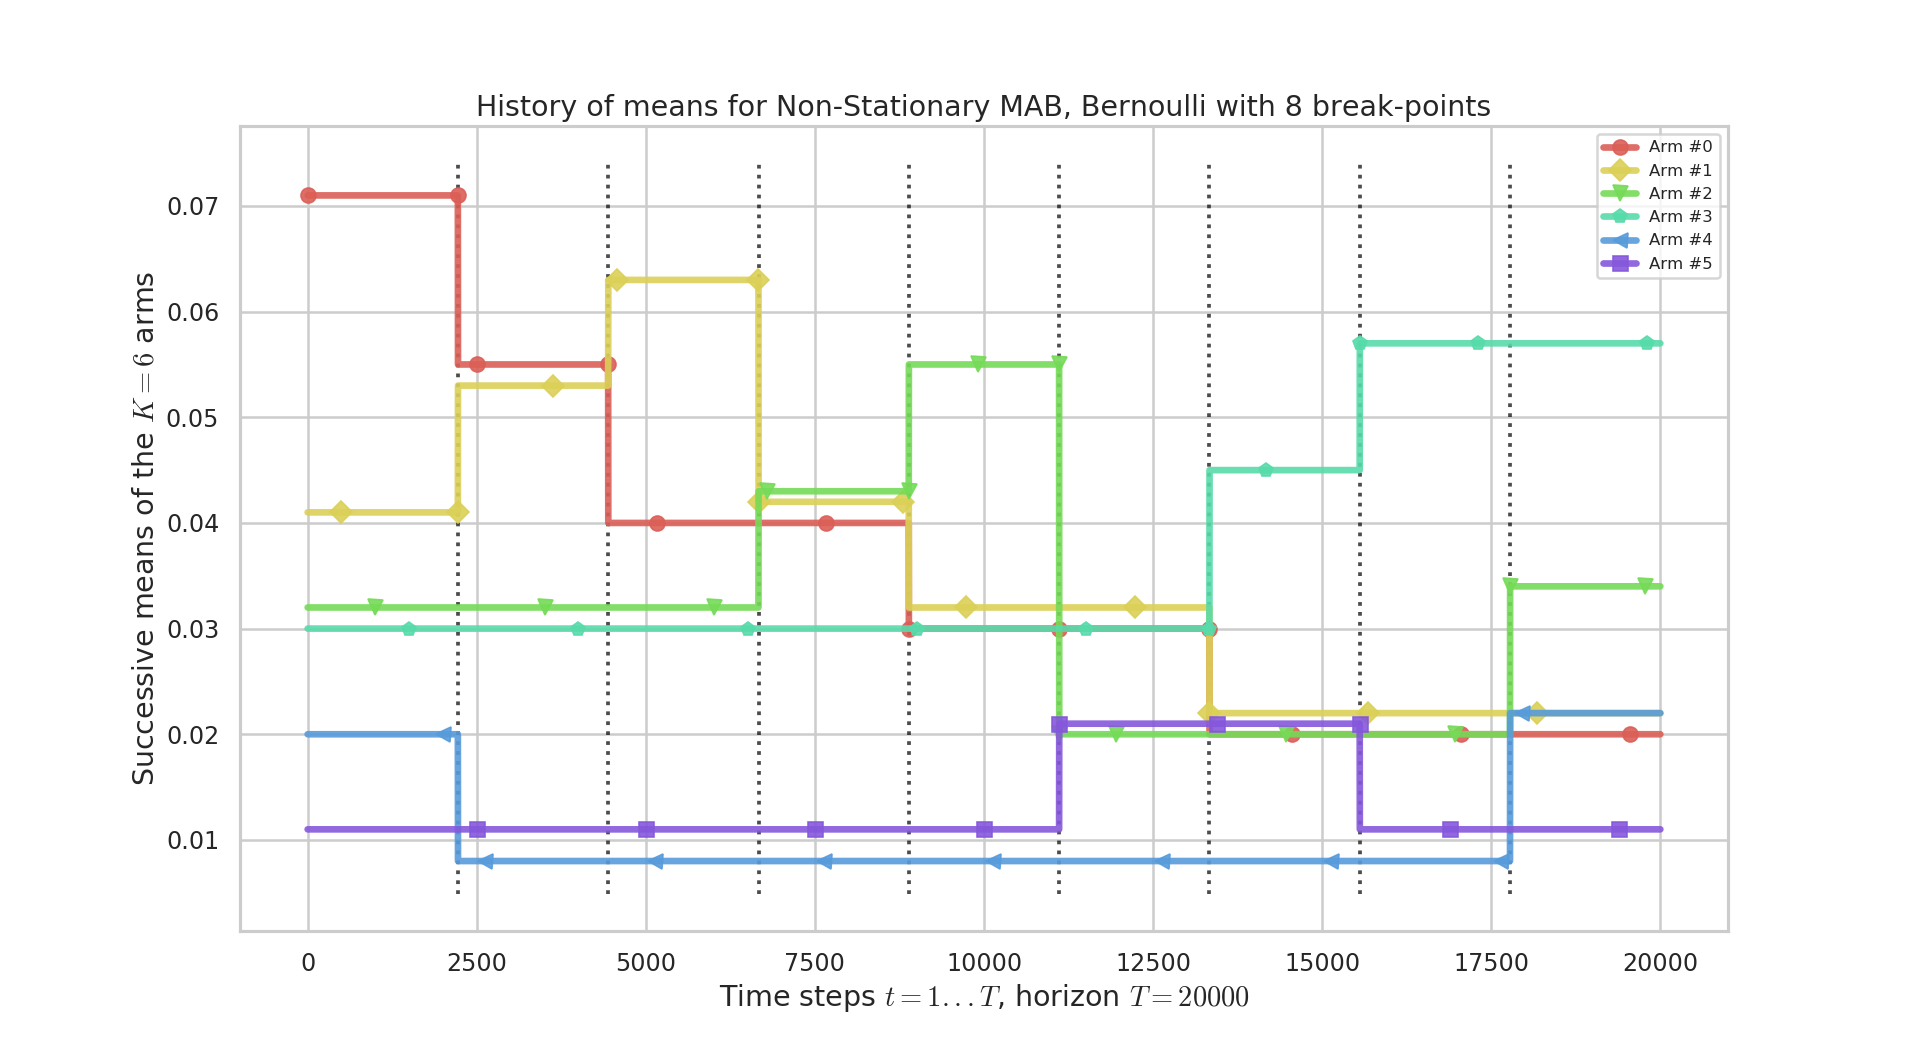
\includegraphics[width=0.80\linewidth]{2-Chapters/6-Chapter/nonstatbandits.git/figures/6_Problems/Problem_5.pdf}
    \caption{\textbf{Problem $3$}: $K=6$, $T=20000$, $C=19$ changes occur on most arms at $\Upsilon=8$ break-points.}
    \label{fig:6:Problem_5}
\end{figure}


% - Pb 4 changes are on all or almost arms at a time, but sequences don't have same length
\paragraph{Problem 4.}

Like problem $1$, it uses $K=3$ arms, $\Upsilon=4$ change-points and $T=5000$,
but the stationary sequences between successive change-points no longer have the same length, as illustrated in Figure~\ref{fig:6:Problem_4}.
Classical (stationary) algorithms such as \klUCB{} can be ``tricked'' by large enough stationary sequences, as they learn with a large confidence the optimal arm, and then fail to adapt to a new optimal arm after a change-point.
We observe below in Table~\ref{table:6:totalResults2} that they can suffer higher regret when the change-points are more spaced out, as this problem starts with a longer stationary sequence of length $T/2$.

\begin{figure}[h!]  % [htbp]
    \centering
    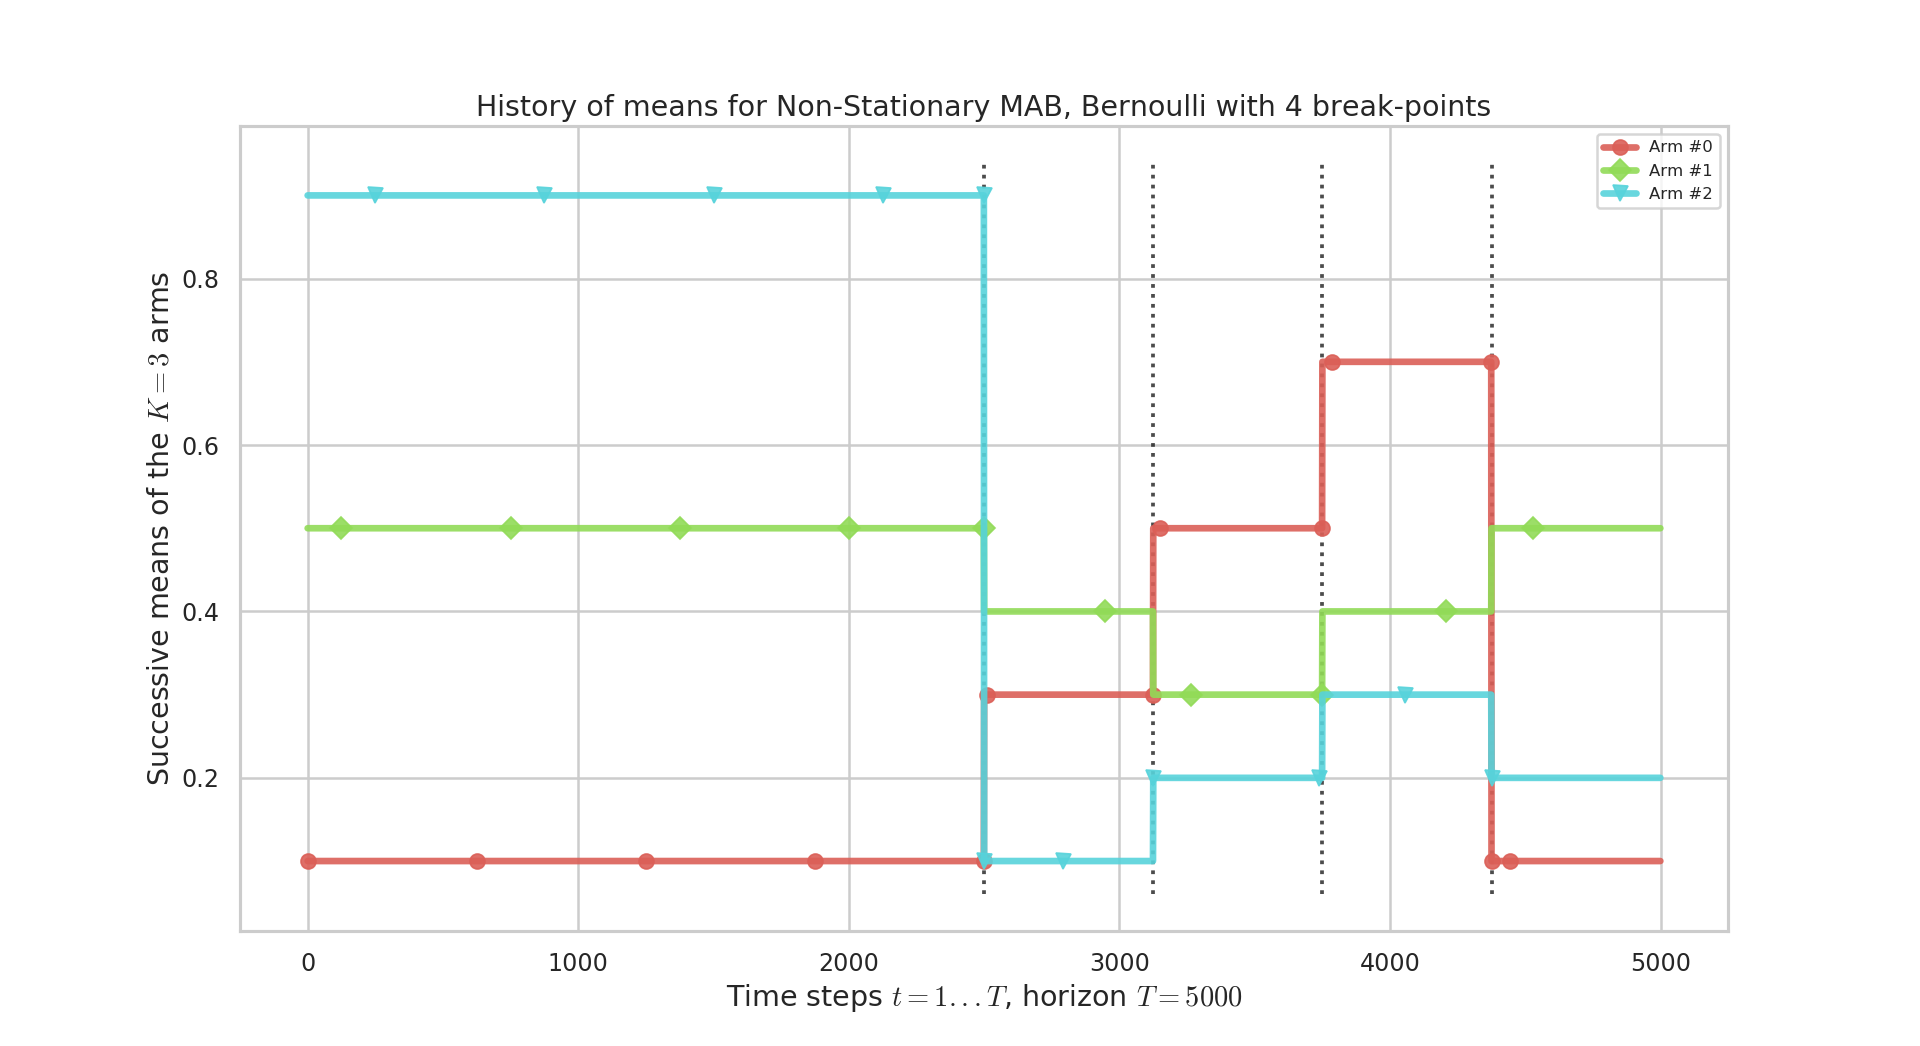
\includegraphics[width=0.80\linewidth]{2-Chapters/6-Chapter/nonstatbandits.git/figures/6_Problems/Problem_4.pdf}
    \caption{\textbf{Problem $4$}: $K=3$, $T=5000$, $C=12$ changes occur on all arms at $\Upsilon=4$ break-points.}
    % \caption{\textbf{Problem 4}: $K=3$ arms with $T=5000$, $\Upsilon=4$ changes occur on all arms at a time (\ie, $C=12$).}
    \label{fig:6:Problem_4}
\end{figure}


% - Pb 6 is Yahoo! example from Figure~3 in CUSUM-UCB paper \cite{LiuLeeShroff17}
\paragraph{Problem 5.}

Like problem $3$, this harder problem is also inspired from synthetic data obtained from a real-world database of clicks from \emph{Yahoo!}, but from another competitor paper, see Figure~3 from \cite{LiuLeeShroff17}.
%
It is much harder, with $\Upsilon=81$ change-points on $K=5$ arms for a longer horizon of $T=100000$.
Some arms change at almost every time steps, for a total number of breakpoints $C=179$, but the optimal arm is almost always the same one (\textcolor{red}{arm $0$, with $\bullet$}).
It is a good benchmark to see if the actively adaptive policies do not detect \emph{too many changes}, as the Oracle-Restart policy suffers higher regret in comparison to \klUCB.
Means are also bounded in $[0.01, 0.07]$, with small gaps of amplitude ranging from $0.02$ to $0.001$,
as shown in Figure~\ref{fig:6:Problem_6}.

\begin{figure}[h!]  % [htbp]
    \centering
    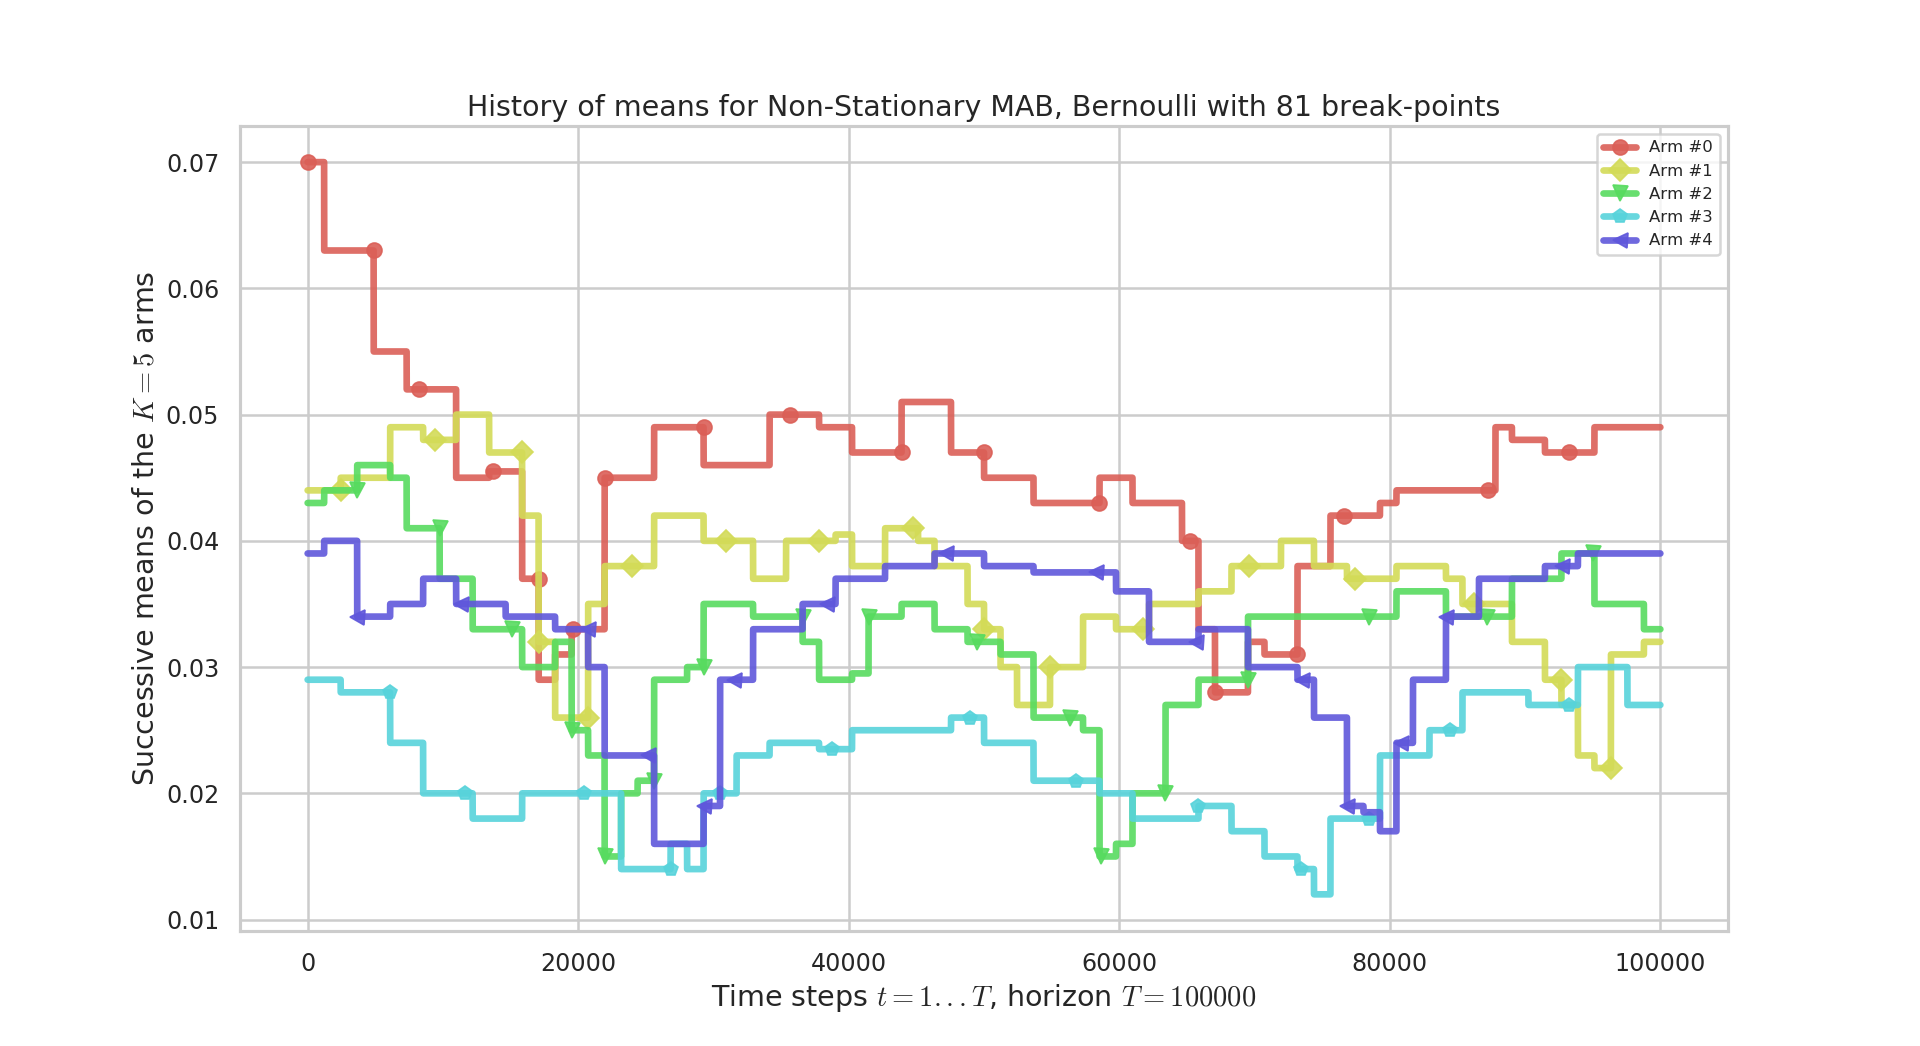
\includegraphics[width=0.80\linewidth]{2-Chapters/6-Chapter/nonstatbandits.git/figures/6_Problems/Problem_6.pdf}
    \caption{\textbf{Problem $5$}: $K=5$, $T=100000$, $C=179$ changes occur on some arms at $\Upsilon=81$ break-points.}
    % \caption{\textbf{Problem 5}: $K=5$, $T=100000$, $\Upsilon=81$ changes occurring on some arms at every time ($C=179$).}
    \label{fig:6:Problem_6}
\end{figure}

% \TODOE{tu as bien tuné CUSUM-UCB avec $\epsilon = 0.02$ dans ce cas?}

% \TODOE{La notion $\Delta^{\text{change}}$ est déjà définie dans la section 4, et ici elle ne veut pas dire la même chose...}


% -----------------------------------------------------------------
\paragraph{Results.}
\label{sub:6:NumericalResults}

% \subsubsection{Results in terms of final regret $R_T$}
% \label{subsub:6:regretPlots}

The two Tables~\ref{table:6:totalResults1} and \ref{table:6:totalResults2} show the final regret $R_T$ obtained for each algorithm.
Results highlighted in \textbf{bold} show the best non-oracle algorithm for each experiments,
with our proposal being the best non-oracle strategy for problems $1$ and $2$.
Thompson sampling and \klUCB{} are efficient,
and better than Discounted-\klUCB{} which is very inefficient.
DTS and SW-\klUCB{} can sometimes be more efficient than their stationary counterparts, but perform worse than the Oracle and most actively adaptive algorithms.
M-\klUCB{} and \CUSUMklUCB{} outperform the previous algorithms, but \GLRklUCB{} is often better.
%
On these problems, \GLRklUCB{} with \textbf{Local} restarts is always more efficient than with \textbf{Global} restarts. Note that on problem 2, all means change at every breakpoint, hence one could expect global restart to be more efficient, yet the experiments show the superiority of local restarts on every instances.

\TODOL{I could add the following algorithms, just to illustrate more:

- OracleRestart with UCB
- M- and CUSUM- with UCB (as defined in the papers)
- Exp3.S
}

\begin{table}[ht]
% \begin{footnotesize}
    \centering
    \begin{tabular}{c|cccccc}
    \textbf{Algorithms} $\;$ \textbackslash $\;$ \textbf{Problems} & Pb $1$ & Pb $2$ & Pb $3$ \\
        \hline
        Oracle-Restart \klUCB{} & $\mathbf{37 \pm 37}$ & $\mathbf{45 \pm 34}$ & $\mathbf{257 \pm 86}$ \\
        \hline
        \klUCB{} & $270 \pm 76$ & $162 \pm 59$ & $529 \pm 148$ \\
        Discounted-\klUCB{} & $1456 \pm 214$ & $1442 \pm 440$ & $1376 \pm 37$ \\
        SW-\klUCB{} & $177 \pm 34$ & $182 \pm 34$ & $1794 \pm 71$ \\
        \hline
        Thompson sampling & $493 \pm 175$ & $388 \pm 147$ & $1019 \pm 245$ \\
        DTS & $209 \pm 38$ & $249 \pm 39$ & $2492 \pm 52$ \\
        \hline
        \MklUCB{} & $290 \pm 29$ & $534 \pm 93$ & $645 \pm 141$ \\
        \CUSUMklUCB{} & $148 \pm 32$ & $152 \pm 42$ & $\mathbf{490 \pm 133}$ \\
        \hline
        \GLRklUCB{}(Local) & $\mathbf{74 \pm 31}$ & $\mathbf{113 \pm 34}$ & $513 \pm 97$ \\
        \GLRklUCB{}(Global) & $97 \pm 32$ & $134 \pm 33$ & $621 \pm 103$
    \end{tabular}
    \caption{Mean regret $\pm$ $1$ std-dev, for different algorithms on problems $1$, $2$ (with $T=5000$) and $3$ ($T=20000$).
    }
    \label{table:6:totalResults1}
% \end{footnotesize}
\end{table}

\begin{table}[ht]
    % \begin{small}
    \centering
    \begin{tabular}{c|cccccc}
        \textbf{Algorithms} $\;$ \textbackslash $\;$ \textbf{Problems} & Pb $4$ ($T=5000$) & Pb $4$ ($T=10000$) & Pb $5$ \\
        \hline
        Oracle-Restart \klUCB{} & $\mathbf{68 \pm 40}$ & $\mathbf{86 \pm 50}$ & $126 \pm 54$ \\
        \hline
        \klUCB{} & $615 \pm 74$ & $1218 \pm 123$ & $106 \pm 36$ \\
        SW-\klUCB{} & $202 \pm 33$ & $322 \pm 47$ & $228 \pm 27$ \\
        Discounted-\klUCB{} & $911 \pm 210$ & $1741 \pm 200$ & $2085 \pm 910$ \\
        \hline
        Thompson sampling & $756 \pm 65$ & $1476 \pm 137$ & $\mathbf{88 \pm 39}$ \\
        DTS & $250 \pm 39$ & $481 \pm 58$ & $238 \pm 24$ \\
        \hline
        \MklUCB{} & $337 \pm 46$ & $544 \pm 47$ & $116 \pm 36$ \\
        \CUSUMklUCB{} & $267 \pm 69$ & $343 \pm 94$ & $117 \pm 34$ \\
        \hline
        \GLRklUCB{}(Local) & $\mathbf{99 \pm 32}$ & $\mathbf{128 \pm 42}$ & $149 \pm 34$ \\
        \GLRklUCB{}(Global) & $128 \pm 32$ & $185 \pm 47$ & $152 \pm 32$
    \end{tabular}
    \caption{Mean regret $\pm$ $1$ std-dev. Problem $4$ use $K=3$ arms, and a first long stationary sequence. Problem $5$ use $K=5$, $T=20000$ and is much harder with $\Upsilon=82$ breakpoints and $C=179$ changes.}
    \label{table:6:totalResults2}
    % \end{small}
\end{table}

One can note that the best non-oracle strategies are actively adaptive,
thus the experiments confirm that an efficient bandit algorithm (\eg, \klUCB) combined with an efficient change point detector (\eg, \GLR) provides efficient strategies for the piece-wise stationary model.


\paragraph{Regret plots.}
\label{subsub:6:regretPlots}

We also include in Appendix~\ref{app:6:moreFigures} some figures showing the simulation results for the five problems.
The results in terms of mean regret $R_T$ are given above in Tables~\ref{table:6:totalResults1} and \ref{table:6:totalResults2}, but it is also interesting to observe two plots for each experiments.
%
First, we show the mean regret as a function of time (\ie, $R_t$ for $1 \leq t \leq T$), for the $9$ algorithms considered (Discounted-\klUCB{} is removed as it is always the most inefficient and suffers high regret).
%
Efficient stationary algorithms, like TS and \klUCB, typically suffer a linear regret after a change on the optimal arm changes if they had ``too'' many samples before the change-points (\eg, on Figure~\ref{fig:6:meanRegretPb1} and even more on Figures~\ref{fig:6:meanRegretPb4} and \ref{fig:6:meanRegretPb5}).
This illustrates the conjecture that classical algorithms can suffer linear regret even on simple piece-wise stationary problems.

On simple problems, like problem $1$, all the algorithms being designed for piece-wise stationary environments perform similarly, but as soon as the gaps are smaller or there is more changes, we clearly observe that our approach \GLRklUCB{} can outperform the two other actively adaptive algorithms \CUSUMklUCB{} and \MklUCB{} (\eg, on Figure~\ref{fig:6:meanRegretPb2}), and performs much more than passively adaptive algorithms DTS and SW-\klUCB{}  (\eg, on Figure~\ref{fig:6:meanRegretPb3}).
Our approach, with the two options of \textbf{Local} or \textbf{Global} restarts, performs very closely to the oracle for problem $4$.

Finally, in the case of hard problems, like problems $3$ and $5$, that have a lot of changes but where the optimal arm barely changes, we verify in Figure~\ref{fig:6:meanRegretPb5} that \klUCB{} and TS can outperform the oracle policy.
Indeed the oracle policy is suboptimal as it restarts as soon as one arm change but is unaware of the meaningful changes, and stationary policies which quickly identify the best arm will play it most of the times, achieving a smaller regret.
We note that, sadly, all actively adaptive policies fail to outperform stationary policies on such hard problems, because they do not observe enough rewards from each arm between two restarts (\ie, the Assumptions~\ref{ass:6:LongPeriodsGlobal} and \ref{ass:6:LongPeriods} for the two Theorems~\ref{thm:6:mainRegretBoundGlobal} and \ref{thm:6:mainRegretBound} are not satisfied).
We can also verify that the two options, \textbf{Local} and \textbf{Global} restart, for \GLRklUCB, give close results, and that the \textbf{Local} option is always better.

We also show the empirical distribution of the regret $R_T$, on Figure~\ref{fig:6:histogramRegretPb1}. It shows that all algorithms have a rather small variance on their regret, except Thompson Sampling which has a large tail due to its large mean regret on this (easy) non-stationary problems.



%----------------------------------------------------------------------------
\section{Conclusion}
\label{sub:6:conclusion}

In this chapter, we studied and presented the piece-wise stationary bandit model, and reviewed existing work.
%
We proposed a new algorithm for this problem, \GLRklUCB, which combines the \klUCB{} algorithm with the Bernoulli GLR change-point detector. This actively adaptive method attains state-of-the-art regret upper-bounds when tuned with a prior knowledge of the number of changes $\Upsilon_T$, but \emph{without any other prior knowledge on the problem}, unlike \CUSUMUCB{} and \MUCB{} that require to know a lower bound on the smallest magnitude of a change. We also gave numerical evidence of the efficiency of our proposal.

We believe that our new proof technique could be used to analyze \GLRklUCB{} under less stringent assumptions than the one made in this chapter (and in previous work), that would require only a few ``meaningful'' changes to be detected. This interesting research direction is left for future work,  but the hope is that the regret would be expressed in term of this number of meaningful changes instead of $\Upsilon_T$. We shall also investigate whether actively adaptive approaches can attain a $\cO(\sqrt{\Upsilon_T T})$ regret upper-bound without the knowledge of $\Upsilon_T$.
We also believe that combining change-point \emph{localization} with an efficient change-point detection algorithm, such as \GLRklUCB, could lead to an interesting class of algorithms, as suggested by \cite{Maillard2018GLR}.
Finally, we would like to study in the future possible extension of our approach to the slowly varying model, as studied in \cite{Besbes14stochastic,WeiSrivastava18Abruptly}.

\TODOL{Evoke here the possibility of study the piece-wise stationary distributed multi-player bandit model introduced in \cite{WeiSrivastava18Distributed} by using \MCTopM{} and \GLRklUCB{} with each other? }

% Finally, we hope that our proposal can be combined with our state-of-the-art $\mathrm{MCTopM}$ algorithm \cite{Besson2018ALT}, to efficiently tackle the piece-wise stationary distributed multi-player bandit model introduced in \cite{WeiSrivastava18Distributed}.


% \paragraph{Acknowledgments.}
% Thanks to Odalric-Ambrym Maillard at Inria Lille for useful discussions, and thanks to Christophe Moy at University Rennes 1.

\paragraph{A note on the simulation code.}
%
All the experiments used for this chapter were performed using SMPyBandits,
and we refer to the following page for details on how to reproduce them,
\href{https://SMPyBandits.GitHub.io/NonStationaryBandits.html}{\texttt{SMPyBandits.GitHub.io/NonStationaryBandits.html}}



% % ----------------------------------------------------------------------------
% \section{Conclusion}
% \label{sec:6:conclusion}

% In this chapter, we saw...

% Future works include...


\newpage
% ----------------------------------------------------------------------------
\section{Appendix}
\label{sec:6:appendix}

We start by including figures as complementary illustrations to the numerical results presented in Section~\ref{sec:6:NumericalExperiments} above.
We then give some additional useful results, along with their proofs, and then we give complementary numerical experiments to justify some choices made in the presentation of our proposal \GLRklUCB.

% -----------------------------------------------------------------
% -----------------------------------------------------------------
\subsection{Additional figures}\label{app:6:moreFigures}
% -----------------------------------------------------------------

We give here plots showing the mean regret $R_t$ as a function of time, and histograms of the distributions of the final regret $R_T$, for the different problems of our benchmark.

Figures~\ref{fig:6:meanRegretPb1} above and \ref{fig:6:histogramRegretPb1} below show that our two proposals are efficient against problem 1.
Then we show similar results for problem 2 in Figure~\ref{fig:6:meanRegretPb2}
and for problem 4 in Figure~\ref{fig:6:meanRegretPb4}.

% -----------------------------------------------------------------
\begin{figure}[h!]  % [htbp]
    \centering
    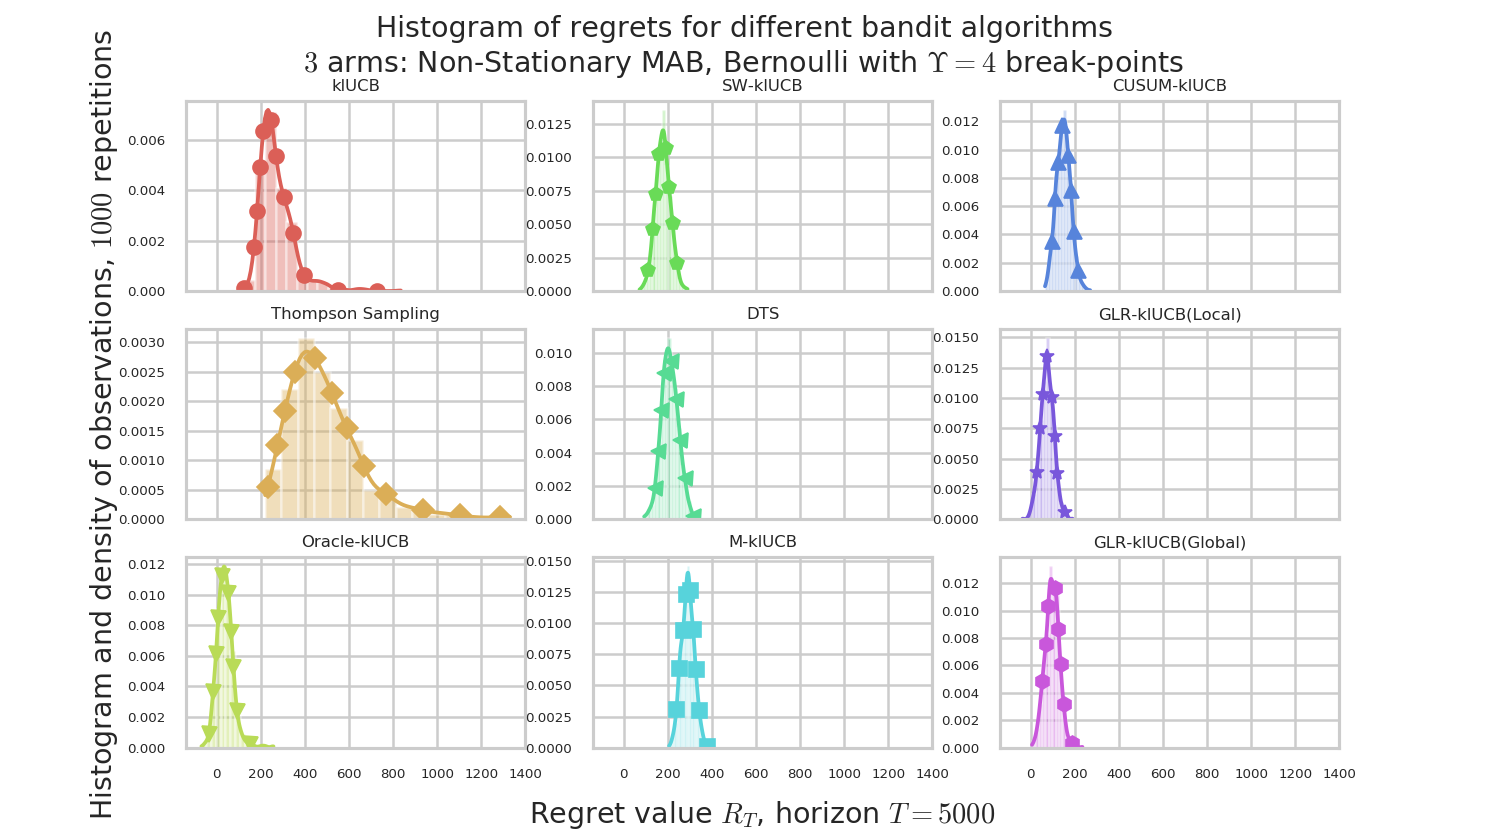
\includegraphics[width=1.09\linewidth]{2-Chapters/6-Chapter/nonstatbandits.git/figures/SP__K3_T5000_N1000__9_algos_pb1/main_HistogramsRegret_shareX____env1-1_1316297932259102962.pdf}
    \caption{Histograms of the distributions of regret $R_T$ ($T=5000$) for problem 1.}
    \label{fig:6:histogramRegretPb1}
\end{figure}

% -----------------------------------------------------------------
\begin{figure}[h!]  % [htbp]
    \centering
    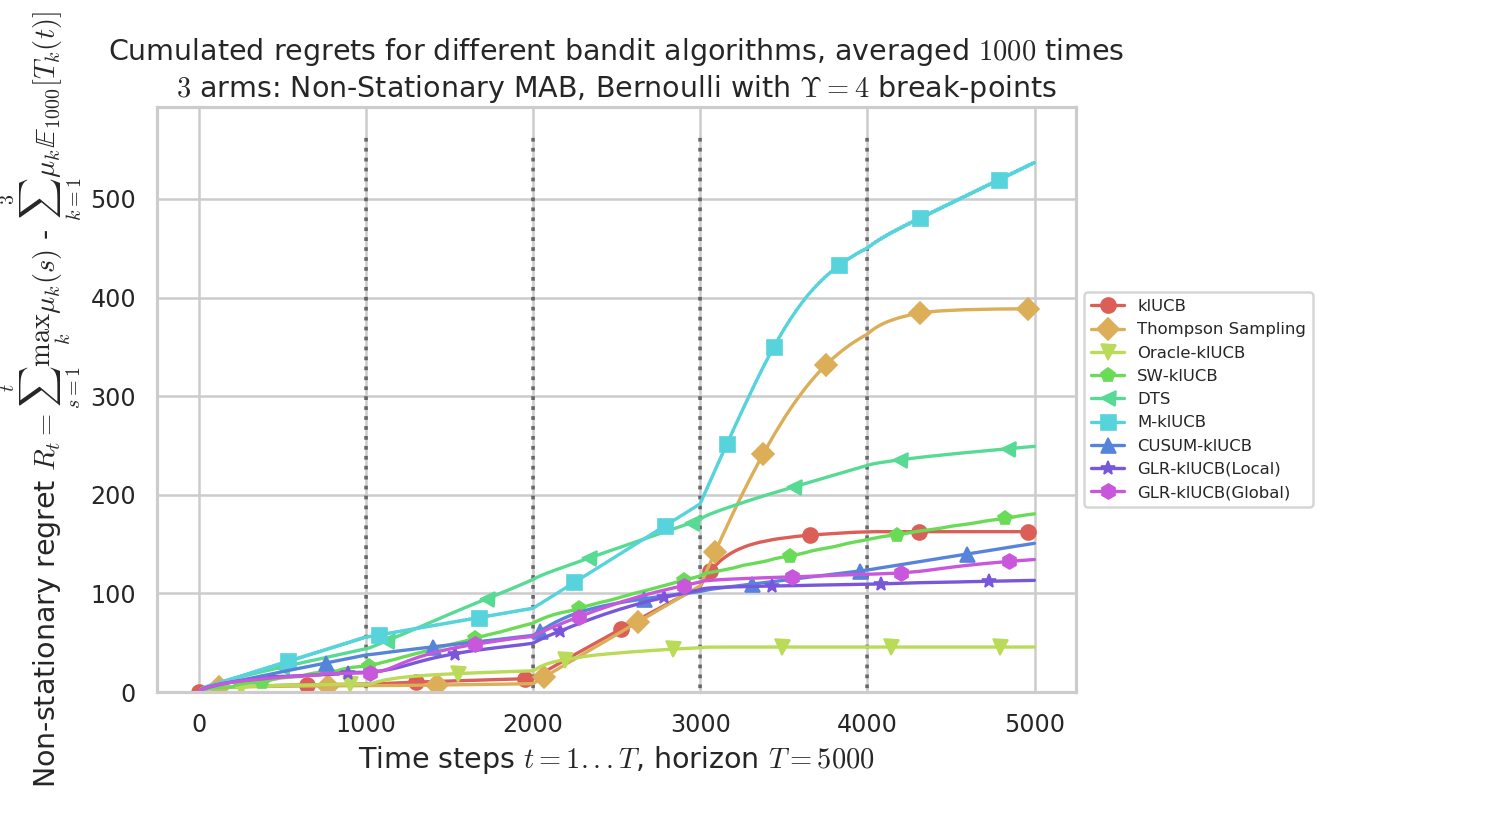
\includegraphics[width=1.09\linewidth]{2-Chapters/6-Chapter/nonstatbandits.git/figures/SP__K3_T5000_N1000__9_algos_pb2/main____env1-1_7882655236216606305.pdf}
    \caption{Mean regret as a function of time, $R_t$ ($1 \leq t \leq T = 5000$) for problem $2$.}
    \label{fig:6:meanRegretPb2}
\end{figure}

% -----------------------------------------------------------------
\begin{figure}[h!]  % [htbp]
    \centering
    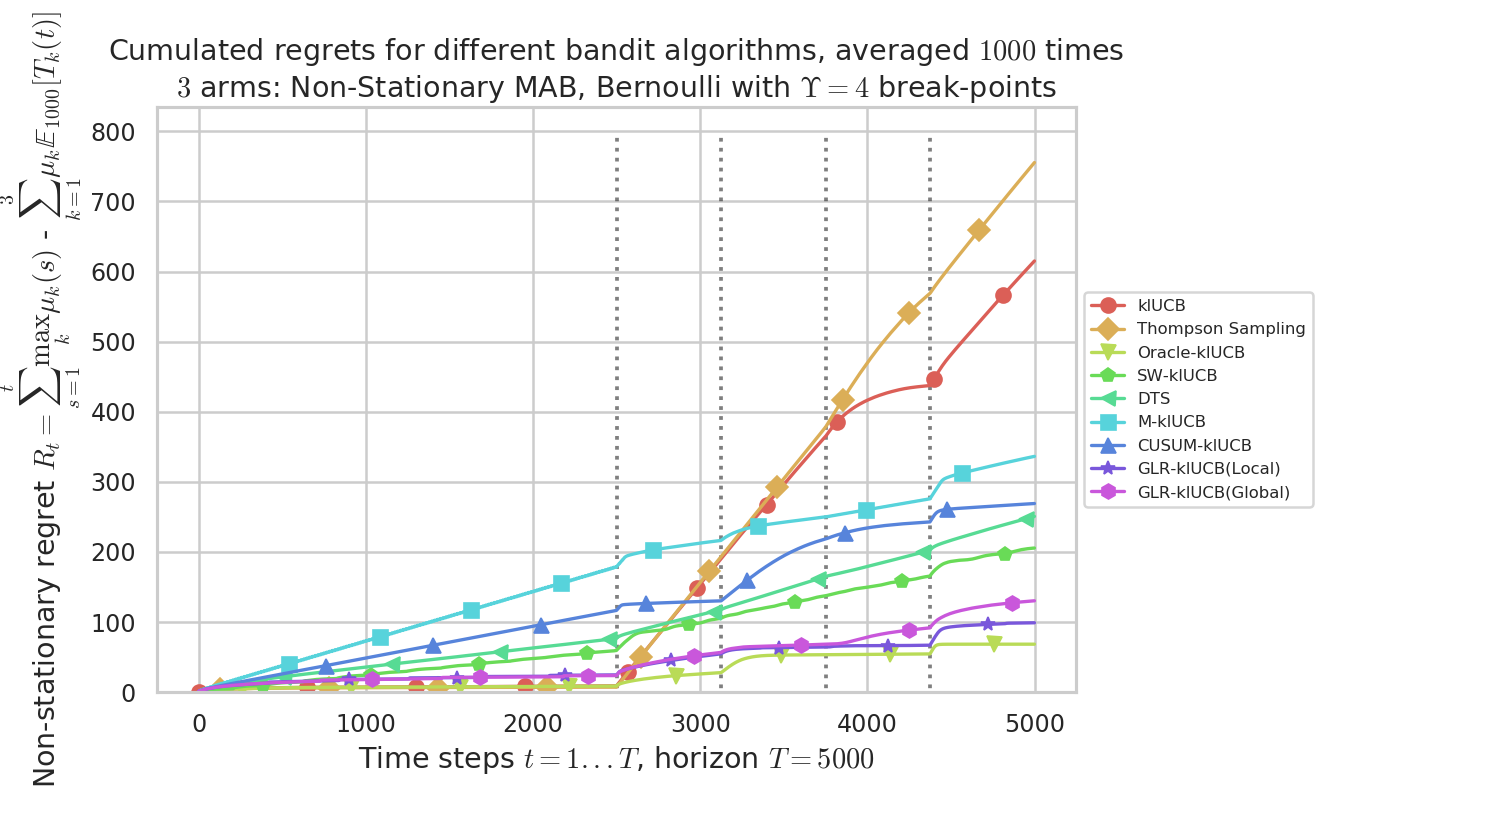
\includegraphics[width=1.09\linewidth]{2-Chapters/6-Chapter/nonstatbandits.git/figures/SP__K3_T5000_N1000__9_algos_pb4/main____env1-1_7471744535647872376.pdf}
    \caption{Mean regret as a function of time, $R_t$ ($1 \leq t \leq T = 5000$) for problem 4.}
    \label{fig:6:meanRegretPb4}
\end{figure}


For harder problems, like problems 3 and 5, the stationary policy \klUCB{} can outperform actively adaptive strategies, if the stationary intervals are too short or if the gap between arms are too small.
In other words, we illustrate in Figures~\ref{fig:6:meanRegretPb3} and \ref{fig:6:meanRegretPb5} that while the actively adaptive strategies can be very efficient when applied to problems that are not too difficult to track, they can become sub-optimal for difficult problems.

% -----------------------------------------------------------------
\begin{figure}[h!]  % [htbp]
    \centering
    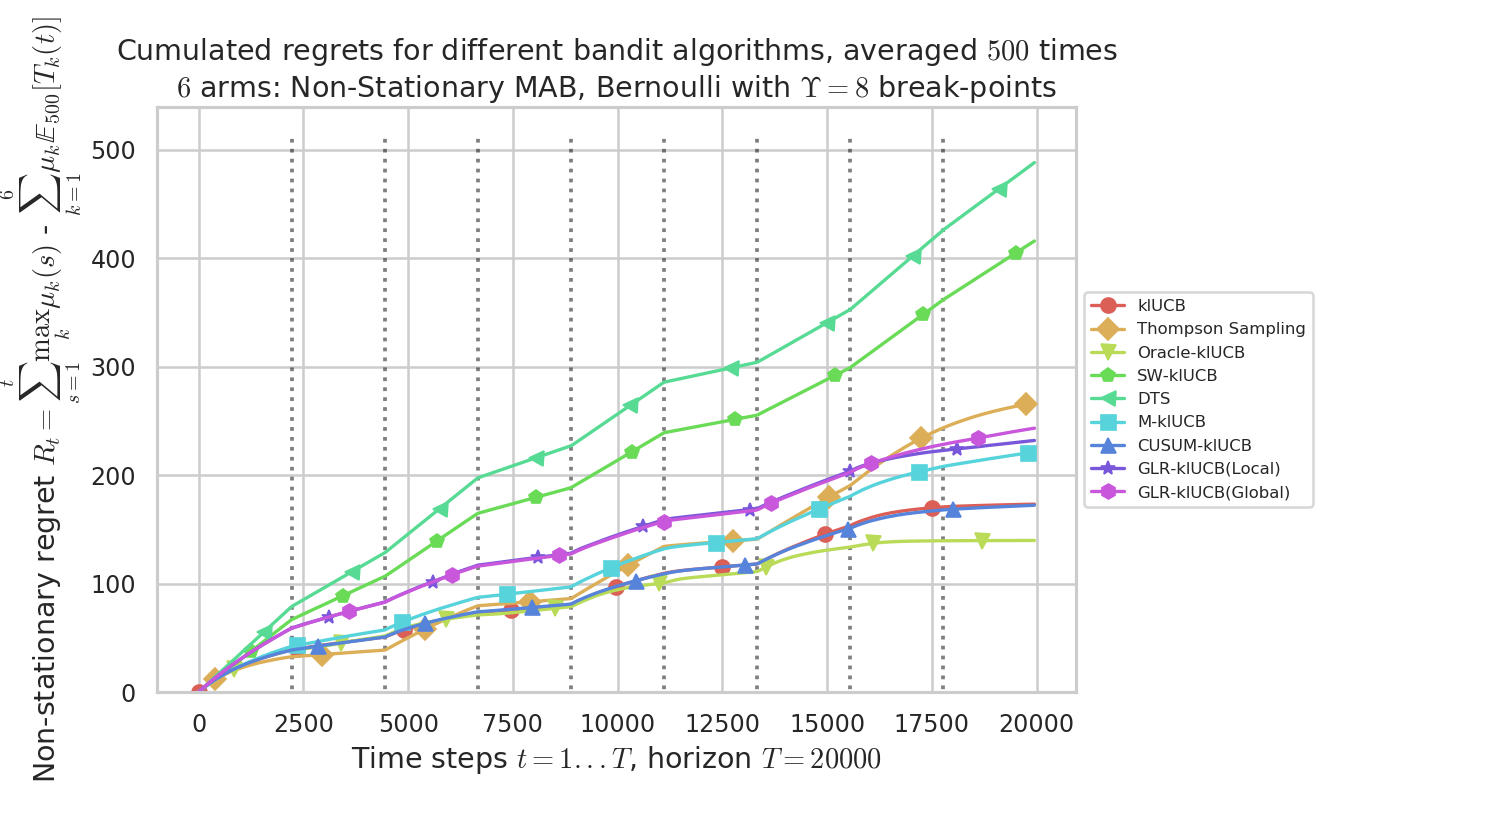
\includegraphics[width=1.09\linewidth]{2-Chapters/6-Chapter/nonstatbandits.git/figures/SP__K6_T20000_N500__9_algos_pb3/main____env1-1_8638317743626238996.pdf}
    \caption{Mean regret as a function of time, $R_t$ ($1 \leq t \leq T = 20000$) for problem 3.}
    \label{fig:6:meanRegretPb3}
\end{figure}


% -----------------------------------------------------------------
\begin{figure}[h!]  % [htbp]
    \centering
    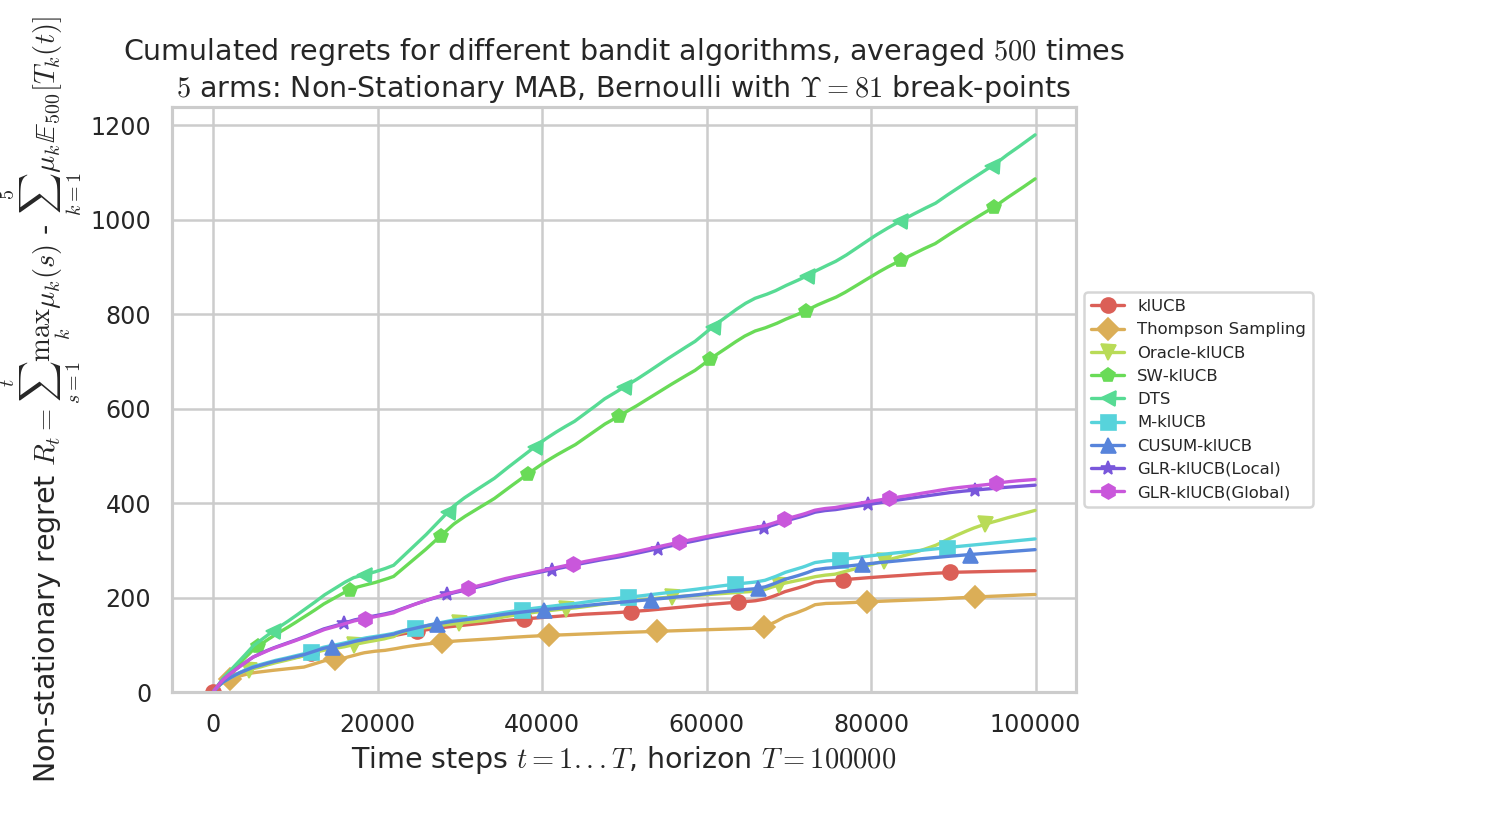
\includegraphics[width=1.09\linewidth]{2-Chapters/6-Chapter/nonstatbandits.git/figures/SP__K5_T100000_N500__9_algos_pb5/main____env1-1_950848333706043320.pdf}
    \caption{Mean regret as a function of time, $R_t$ ($1 \leq t \leq T = 100000$) for problem 5.}
    \label{fig:6:meanRegretPb5}
\end{figure}


% ----------------------------------------------------------------------------
% ----------------------------------------------------------------------------
\subsection{Omitted proofs}\label{proof:6:Conc}
% ----------------------------------------------------------------------------

This Appendix gives some proofs omitted in the main text of this chapter.
Missing proofs can be found in the article \cite{Besson2019GLRT}.



% % ----------------------------------------------------------------------------
% \subsubsection{Simplified expression for the GLR statistic}\label{app:6:GLR_with_kl}

% % Remember that the Generalized Likelihood Ratio statistic for the test presented in \eqref{eq:6:firstDefGLRT} in Section~\ref{sub:6:presentationOfGLRTest} is
% % \[\GLR(n) := \frac{\sup\limits_{\mu_0,\mu_1,\tau < n}\ell(X_1, \ldots, X_n ; \mu_0,\mu_1,\tau)}{\sup\limits_{\mu_0}\ell(X_1, \ldots, X_n ; \mu_0)},\]
% % %
% % where $\ell(X_1, \ldots, X_n ; \mu_0)$ and $\ell(X_1, \ldots, X_n ; \mu_0,\mu_1,\tau)$ respectively denote the likelihoods of the first $n$ observations under a model in $\cH_0$ and $\cH_1$.

% The Generalized Likelihood Ratio statistic for the test is presented above in \eqref{eq:6:firstDefGLRT} in Section~\ref{sub:6:presentationOfGLRTest}.
% %
% We refer to \cite{Basseville93} and reference therein for the generic proof, but we prove here the specific case of Bernoulli distributions.
% % For any $k \leq k'$, we denote $\widehat{\mu}_{k:k'} := \frac{1}{k - k' + 1} \sum_{l=k}^{k'} X_l$ denotes the average of the observations $X_l$ collected between the instants $k$ and $k'$.
% %
% We prove below that the GLR test is equivalent to
% \begin{align*}
%     \GLR(n)
%     &= \frac{\sup\limits_{\mu_0,\mu_1,\tau < n}\ell(X_1, \ldots, X_n ; \mu_0,\mu_1,\tau)}{\sup\limits_{\mu_0}\ell(X_1, \ldots, X_n ; \mu_0)} \\
%     &= \exp\Bigl[ \sup_{s \in [2,n-1]} \left[s \times \kl\left(\widehat{\mu}_{1:s},\widehat{\mu}_{1:n}\right) + (n-s) \times \kl\left(\widehat{\mu}_{s+1:n},\widehat{\mu}_{1:n}\right)\right] \Bigr].
% \end{align*}
% %
% % Remember that the binary relative entropy $\kl$, defined for $x,y\in[0,1]$
% % by $\kl(x,y) := x \ln\left(\frac{x}{y}\right) + (1-x)\ln\left(\frac{1-x}{1-y}\right)$,
% % with the usual convention that $t \log(t) = 0$ if $t=0$.

% \begin{proof}
%     First, we consider the denominator in the expression of $\GLR(n)$ \eqref{eq:6:firstDefGLRT}, that is the $\sup$ on $\mu_0$.
%     We have $\ell(X_1, \ldots, X_n ; \mu_0) = \prod_{i=1}^n \ell(X_i ; \mu_0)$ by independence of the observations $X_i$,
%     and $\ell(X_i ; \mu_0) = \mu_0^{X_i} (1-\mu_0)^{1-X_i}$ for Bernoulli distributions.
%     Therefore, taking the logarithm gives
%     \begin{align*}
%         \log\ell(X_1, \ldots, X_n ; \mu_0)
%         &= \sum_{i=1}^n X_i \log(\mu_0) + (1-X_i) \log(1-\mu_0) \\
%         &= \log(\mu_0) \times \left( \sum_{i=1}^n X_i \right) + \log(1-\mu_0) \times \left( n - \sum_{i=1}^n X_i \right) \\
%         &= n \left[ \widehat{\mu}_{1:n} \log(\mu_0) + (1 - \widehat{\mu}_{1:n}) \log(1-\mu_0) \right].
%     \end{align*}
%     %
%     For a constant $a\in[0,1]$, let $h(x) := a \log(x) + (1-a) \log(1-x)$ on $(0,1)$,
%     and we are trying to solve $\sup_{x\in[0,1]} h(x)$.
%     If $a=0$ or $a=1$, $h$ is maximum at $x=a$.
%     Now if $a\neq0$, As $h$ is of class $\cC^1$, we can just differentiate and find the root of its derivative:
%     $h'(x) = a/x - (1-a)/(1-x)$, so $h'(x) = 0$ if and only if $x=a$.
%     Thus in all cases, $\sup_{x\in[0,1]} h(x) = h(a)$.
%     %
%     Here, we have $a = \widehat{\mu}_{1:n}$, and thus we solve the $\sup_{\mu_0}$ optimization problem found in the denominator of the $\GLR(n)$ expression.
%     By replacing $\mu_0 = \widehat{\mu}_{1:n}$, we obtained the following (unique) solution,
%     \begin{equation}\label{eq:6:solutionPbOpt_for_1n}
%         \sup_{\mu_0} \log\ell(X_1, \ldots, X_n ; \mu_0) = n \left( \widehat{\mu}_{1:n} \log(\widehat{\mu}_{1:n}) + (1 - \widehat{\mu}_{1:n}) \log(1-\widehat{\mu}_{1:n}) \right).
%     \end{equation}

%     Now let us consider the nominator of the $\GLR(n)$ expression.
%     We can again work with log-likelihoods, and so we have
%     \begin{align*}
%         \log\ell(X_1, \ldots, X_n ; \mu_0,\mu_1,\tau)
%         &= \sum_{i=1}^{\tau} X_i \log(\mu_0) + (1-X_i) \log(1-\mu_0) + \sum_{i=\tau+1}^n X_i \log(\mu_1) + (1-X_i) \log(1-\mu_1) \\
%         &= s \bigl( \widehat{\mu}_{1:s} \log(\mu_0) + (1 - \widehat{\mu}_{1:s}) \log(1-\mu_0) \bigr) \\
%         & \;\;\;\; + (n-s) \bigl( \widehat{\mu}_{s+1:n} \log(\mu_1) + (1 - \widehat{\mu}_{s+1:n}) \log(1-\mu_1) \bigr).
%     \end{align*}
%     Because we solved in \eqref{eq:6:solutionPbOpt_for_1n} the $\sup$ for the denominator,
%     we have
%     \begin{align*}
%         \GLR(n)
%         % &= \frac{\sup\limits_{\mu_0,\mu_1,\tau < n}\ell(X_1, \ldots, X_n ; \mu_0,\mu_1,\tau)}{\sup\limits_{\mu_0}\ell(X_1, \ldots, X_n ; \mu_0)}, \\
%         &= \frac{\sup\limits_{\mu_0,\mu_1,\tau < n}\ell(X_1, \ldots, X_n ; \mu_0,\mu_1,\tau)}{ \exp\left[ n \left( \widehat{\mu}_{1:n} \log(\mu_0) + (1 - \widehat{\mu}_{1:n}) \log(1-\mu_0) \right) \right] }, \\
%         &= \sup\limits_{\mu_0,\mu_1,\tau < n} \frac{\ell(X_1, \ldots, X_n ; \mu_0,\mu_1,\tau)}{ \exp\left[ n \left( \widehat{\mu}_{1:n} \log(\widehat{\mu}_{1:n}) + (1 - \widehat{\mu}_{1:n}) \log(1-\widehat{\mu}_{1:n}) \right) \right] }, \\
%         &= \exp \Bigl[ \sup\limits_{\mu_0,\mu_1,\tau < n} \Bigl[ \log\Bigl[ \frac{\ell(X_1, \ldots, X_n ; \mu_0,\mu_1,\tau)}{ \exp\left[ n \left( \widehat{\mu}_{1:n} \log(\widehat{\mu}_{1:n}) + (1 - \widehat{\mu}_{1:n}) \log(1-\widehat{\mu}_{1:n}) \right) \right] } \Bigr] \Bigr] \Bigr],  \\
%         &= \exp \Bigl[ \sup\limits_{\mu_0,\mu_1, 1 < s < n} \Bigl[
%             s \bigl( \widehat{\mu}_{1:s} \log(\mu_0) + (1 - \widehat{\mu}_{1:s}) \log(1-\mu_0) \bigr) \\
%             & \hspace{35pt} + (n-s) \bigl( \widehat{\mu}_{s+1:n} \log(\mu_1) + (1 - \widehat{\mu}_{s+1:n}) \log(1-\mu_1) \bigr) \\
%             & \hspace{35pt} - n \bigl( \widehat{\mu}_{1:n} \log(\widehat{\mu}_{1:n}) + (1 - \widehat{\mu}_{1:n}) \log(1-\widehat{\mu}_{1:n}) \bigr)
%         \Bigr] \Bigr].
%     \end{align*}
%     By linearity and independence, we can separate the joint optimization problem on $\mu_0,\mu_1,s$ in two optimizations problems for $\mu_0,s$ and $\mu_1,s$, that can first be solved explicitly for $\mu_0$ (resp. $\mu_1$) and then left to be solved for $s$.
%     By definition, $n \; \widehat{\mu}_{1:n} = \sum_{i=1}^n X_i = s \;\widehat{\mu}_{1:s} + (n-s) \;\widehat{\mu}_{s+1:n}$, so the right hand side (negative) part involving $\widehat{\mu}_{1:n}$ can be distributed in the two left hand side (positive) terms,
%     which are both handled similarly.
%     For instance for $\mu_0$, we use the same computation as above with the function $h$ to find the optimum:
%     $\widehat{\mu}_{1:s} \log(\mu_0) + (1 - \widehat{\mu}_{1:s}) \log(1-\mu_0)$
%     is optimum for $\mu_0 = \widehat{\mu}_{1:s}$.
%     Similarly, the term for $\mu_1$ gives that $\sup_{\mu_1} \widehat{\mu}_{s+1:n} \log(\mu_1) + (1 - \widehat{\mu}_{s+1:n}) \log(1-\mu_1)$
%     is attained for $\mu_1 = \widehat{\mu}_{s+1:n}$.
%     Finally, by replacing the two expressions of the solutions for $\mu_0$ and $\mu_1$,
%     we obtain
%     \begin{align*}
%         \GLR(n)
%         = \exp \Bigl[ \sup\limits_{1 < s < n} \Bigl[
%             s \times \Bigl(
%                     & \widehat{\mu}_{1:s} \log(\widehat{\mu}_{1:s}) + (1 - \widehat{\mu}_{1:s}) \log(1-\widehat{\mu}_{1:s}) \\
%                     & - \widehat{\mu}_{1:s} \log(\widehat{\mu}_{1:n}) + (1 - \widehat{\mu}_{1:s}) \log(1-\widehat{\mu}_{1:n})
%             \Bigr) \\
%             + (n-s) \times \Bigl(
%                 & \widehat{\mu}_{s+1:n} \log(\widehat{\mu}_{s+1:n}) + (1 - \widehat{\mu}_{s+1:n}) \log(1-\widehat{\mu}_{s+1:n}) \\
%                 & - \widehat{\mu}_{s+1:n} \log(\widehat{\mu}_{1:n}) + (1 - \widehat{\mu}_{s+1:n}) \log(1-\widehat{\mu}_{1:n})
%             \Bigr)
%         \Bigr] \Bigr].
%     \end{align*}
%     We conclude by recognizing the expressions of $s \times \kl(\widehat{\mu}_{1:s}, \widehat{\mu}_{1:n})$
%     and $(n-s) \times \kl(\widehat{\mu}_{s+1:n}, \widehat{\mu}_{1:n})$.
% \end{proof}


% Consider $(Y_i)_{i\in\N}$ some data, and $t_0\in\N$, $t\in\N$ and any $s\in[t_0,t)$.
% For any $a<b$, define $\mu_{a:b} := \frac{1}{b-a+1} \sum_{i=a}^{b} Y_i$ the mean of samples from $a$ to $b$.

% In a one dimensional exponential family, \eg, Gaussian distributions of known variance ($\sigma=1$) or Bernoulli distributions, the Kullback-Leibler divergence of two distributions is expressed with a $\kl$ function of their mean.
% That is, for two distributions $\nu_1,\nu_2$ of means $\mu_1,\mu_2$,
% $$\KL(\nu_1,\nu_2) = \kl(\mu_1,\mu_2).$$

% The \GLR{} test is defined in \cite{Maillard2018GLR}, and is written like this.
% $$\GLR^{\kl}_{t_0 : s : t} = (s-t_0+1) \kl(\mu_{t_0:s}, \mu_{t_0:t}) + (t-s) \kl(\mu_{s+1:t}, \mu_{t_0:t}).$$

% \begin{lemma}[Simplified expression for $\GaussianGLR$]\label{lem:XXX}
%     For $\cN_1$, the exponential family of Gaussian distributions of variance $\sigma^2=1$,
%     the \GLR{} test can be simplified:
%     \begin{align}
%         \forall t_0 \leq s < t,\; \GaussianGLR_{t_0 : s : t} &= (s-t_0+1) \kl(\mu_{t_0:s}, \mu_{t_0:t}) + (t-s) \kl(\mu_{s+1:t}, \mu_{t_0:t})\\
%         &= \frac{(s-t_0+1)(t-s)}{t-t_0+1} \kl(\mu_{s+1:t}, \mu_{t_0:s}) = \frac{(s-t_0+1)(t-s)}{t-t_0+1} \frac{(\mu_{s+1:t}, \mu_{t_0:s})^2}{2}.
%     \end{align}
% \end{lemma}
% \begin{proof}
%     Define $k_1 := \kl(\mu_{t_0:s}, \mu_{t_0:t})$,
%     $k_2 := \kl(\mu_{s+1:t}, \mu_{t_0:t})$,
%     and $k_3 := \kl(\mu_{s+1:t}, \mu_{t_0:s})$.
%     In this family $\cN_1$, $\kl(x,y) = \frac{(x-y)^2}{2}$. Let us multiply everything by $2$ to avoid having this $\frac{1}{2}$ on every line.
%     % \begin{small}
%     \begin{align*}
%         &2 (s-t_0+1) k_1 + (t-s) k_2 \\
%         &=
%         (s-t_0+1)\mu_{t_0:s}^2 + (t-s)\mu_{s+1:t}^2 + (s-t_0+1+t-s)\mu_{t_0:t}^2 \\
%         &\;\;\;\;\;\;\;\;\;- 2 (s-t_0+1)\mu_{t_0:s}\mu_{t_0:t}
%         - 2 (t-s)\mu_{s+1:t}\mu_{t_0:t} \\
%         &= (s-t_0+1)\mu_{t_0:s}^2 + (t-s)\mu_{s+1:t}^2 + (t-t_0+1)\mu_{t_0:t}^2 \\
%         &\;\;\;\;\;\;\;\;\;- 2 (\underbrace{(s-t_0+1)\mu_{t_0:s}+(t-s)\mu_{s+1:t}}_{=\sum_{i=t_0}^{t} Y_i = (t-t_0+1) \mu_{t_0:t}})\mu_{t_0:t} \\
%         &= (s-t_0+1)\mu_{t_0:s}^2 + (t-s)\mu_{s+1:t}^2 - (t-t_0+1)\mu_{t_0:t}^2 \\
%         &= \frac{\left(\sum_{i=t_0}^{s} Y_i \right)^2}{s-t_0+1} + \frac{\left(\sum_{i=s+1}^{t} Y_i \right)^2}{t-s} - \frac{\left(\sum_{i=t_0}^{t} Y_i \right)^2}{t-t_0+1} \\
%         &= \frac{1}{t-t_0+1} \Bigl( \frac{(s-t_0+1) + (t-s)}{s-t_0+1} \left(\sum_{i=t_0}^{s} Y_i \right)^2 + \frac{(s-t_0+1) + (t-s)}{t-s} \left(\sum_{i=s+1}^{t} Y_i \right)^2 \\
%         &\;\;\;\;\;\;\;\;\;- \left(\sum_{i=t_0}^{s} Y_i + \sum_{i=s+i}^{t} Y_i \right)^2 \Bigr) \\
%         &= \frac{1}{t-t_0+1} \Bigl( \left(\sum_{i=t_0}^{s} Y_i \right)^2 + \frac{t-s}{s-t_0+1} \left(\sum_{i=t_0}^{s} Y_i \right)^2 + \left(\sum_{i=s+1}^{t} Y_i \right)^2 + \frac{s-t_0+1}{t-s} \left(\sum_{i=s+1}^{t} Y_i \right)^2 \\
%         &\;\;\;\;\;\;\;\;- \left(\sum_{i=t_0}^{s} Y_i \right)^2 - \left(\sum_{i=s+i}^{t} Y_i \right)^2 - 2 \left(\sum_{i=t_0}^{s} Y_i \right) \left(\sum_{i=s+i}^{t} Y_i \right) \Bigr) \\
%         &= \frac{1}{t-t_0+1} \Bigl(\frac{t-s}{s-t_0+1} \left(\sum_{i=t_0}^{s} Y_i \right)^2 + \frac{s-t_0+1}{t-s} \left(\sum_{i=s+1}^{t} Y_i \right)^2 - 2 \left(\sum_{i=t_0}^{s} Y_i \right) \left(\sum_{i=s+i}^{t} Y_i \right) \Bigr) \\
%         &= \frac{(s-t_0+1)(t-s)}{t-t_0+1} \Bigl( \frac{1}{(s-t_0+1)^2} \left(\sum_{i=t_0}^{s} Y_i \right)^2 + \frac{1}{(t-s)^2} \left(\sum_{i=s+1}^{t} Y_i \right)^2 \\
%         &\;\;\;\;\;\;\;\;\;- 2 \left(\frac{1}{s-t_0+1} \sum_{i=t_0}^{s} Y_i \right) \left(\frac{1}{t-s} \sum_{i=s+1}^{t} Y_i \right) \Bigr) \\
%         &= \frac{(s-t_0+1)(t-s)}{t-t_0+1} (\mu_{s+1:t} - \mu_{t_0:s})^2 = 2 \frac{(s-t_0+1)(t-s)}{t-t_0+1} k_3.
%     \end{align*}
%     as wanted.
%     % \end{small}
% \end{proof}

% This is not true for all one dimensional exponential family, for instance for Bernoulli distributions it is almost never the case.
% Imagine $t_0=0, t=2, s=1$ and data $Y_i = [0,1]$.
% Then $\mu_{t_0:s}=0$, $\mu_{s+1:t}=1$, $\mu_{t_0:t}=0.5$, and so $k_1 = \kl(0,0.5) = \log(2)$ and $k_2 = \kl(1,0.5)=\log(2)$ and $k_3=\kl(0,1)=-\infty$ so we do not have
% $(s-t_0+1) \kl(\mu_{t_0:s}, \mu_{t_0:t}) + (t-s) \kl(\mu_{s+1:t}, \mu_{t_0:t}) = \frac{(s-t_0+1)(t-s)}{t-t_0+1} \kl(\mu_{s+1:t}, \mu_{t_0:s})$.



% ----------------------------------------------------------------------------
\subsubsection{Proof of Lemma~\ref{lem:6:ConcFirst}.}
\label{app:6:proofConcFirst}
%
Using the same construction as in the proof of Theorem~14 in \cite{KK18Martingales}, one can prove that for every $\lambda \in I$ (for an interval $I$), there exists a non-negative super-martingale $M^\lambda (s)$ with respect to the filtration $\cF_t = \sigma(X_1,\dots,X_t)$ that satisfies $\bE[M^\lambda(s)] \leq 1$ and
\[\forall s \in \N^*, \ \ M^\lambda (s) \geq \mathrm{e}^{\lambda [s \, \kl(\widehat{\mu}_s,\mu) - 3\ln(1+\ln(s))] - g(\lambda)}\]
for some function $g : I \rightarrow \R$. This super-martingale is of the form
$M^\lambda (s) = \int \mathrm{e}^{\eta\sum_{i=1}^s X_i - \phi_\mu(\lambda)s} d\pi(\eta)$,
for a well-chosen probability distribution $\pi$, and the function $g$ can be chosen to be any
\begin{eqnarray*}
    g_{\xi} : \left[0; 1/(1+\xi)\right] & \longrightarrow & \R \\
    \lambda & \mapsto & \lambda(1+\xi) \ln \left(\frac{\pi^2}{3(\ln(1+\xi))^2}\right) -  \ln(1 - \lambda(1 + \xi))
\end{eqnarray*}
for a parameter $\xi \in [0,1/2]$.

Similarly, there exists an independent super-martingale $W^\lambda (r)$ w.r.t. the filtration $\cF_r' = \sigma(Y_1,\dots,Y_r)$ such that
\[\forall r \in \N^*, \ \ W^\lambda (r) \geq \mathrm{e}^{\lambda [r\kl(\widehat{\mu}'_r,\mu) - 3\ln(1+\ln(r))] - g(\lambda)},\]
for the same function $g(\lambda)$.
In the terminology of \cite{KK18Martingales}, the processes $\bm{X}(s) = s \, \kl(\widehat{\mu}_s,\mu) - 3\ln(1+\ln(s))$ and $\bm{Y}(s) = r \, \kl(\widehat{\mu}_r,\mu) - 3\ln(1+\ln(r))$ are called $g$-DCC for Doob-Cram\'er-Chernoff, as Doob's inequality can be applied in combination with the Cram\'er-Chernoff method to obtain deviation inequalities that are uniform in time.

Here we have to modify the technique used in their Lemma 4 in order to take into account the two stochastic processes, and the presence of super-martingales instead of martingales (for which Doob inequality still works).
One can write
%
\begin{align*}
    &\bP\bigl( \exists r \in \N^* : s \, \kl\left(\widehat{\mu}_{s},\mu\right) + r \, \kl\left(\widehat{\mu}_r',\mu'\right) > 3\ln(1+\ln(s)) + 3\ln(1+\ln(r)) + u \bigr) \\
    & \leq \bP\left(\exists r \in \N^* : M^\lambda(s)W^\lambda(r) > \mathrm{e}^{\lambda u - 2g(\lambda)}\right) \\
    & = \lim_{n \rightarrow \infty} \bP\left(\exists r \in [n] :  M^\lambda(s)W^\lambda(r) > \mathrm{e}^{\lambda u - 2g(\lambda)}\right) \\
    & = \lim_{n \rightarrow \infty} \bP\left(\sup_{r \in [n]}  M^\lambda(s)W^\lambda(r) > \mathrm{e}^{\lambda u - 2g(\lambda)}\right).
\end{align*}
%
Using that $\tilde{M}(r) = M^\lambda(s)W^\lambda(r)$ is a super-martingale with respect to the filtration $\tilde{\cF}_r = \sigma(X_1,\dots,X_s, Y_1,\dots,Y_r)$, one can apply Doob's maximal inequality to obtain
\begin{eqnarray*}
    \bP\left(\sup_{r \in [n]}  M^\lambda(s)W^\lambda(r) > \mathrm{e}^{\lambda u - 2g(\lambda)}\right) &\leq& \mathrm{e}^{-(\lambda u - 2g(\lambda))}\bE[\tilde{M}(1))] \\
    & = & \mathrm{e}^{-(\lambda u - 2g(\lambda))}\bE[M^\lambda(s)W^\lambda(1)] \\
    & \leq & \mathrm{e}^{-(\lambda u - 2g(\lambda))},
\end{eqnarray*}
using that $M^\lambda(s)$ and $W^\lambda(1)$ are independent and have an expectation smaller than $1$.

Putting things together yields
\[\bP\left(\exists r \in \N^* : s \, \kl\left(\widehat{\mu}_{s},\mu\right) + r \, \kl\left(\widehat{\mu}_r',\mu'\right) > 3\ln(1+\ln(s)) + 3\ln(1+\ln(r)) + u\right) \leq \mathrm{e}^{-\left(\lambda u - 2g_{\xi}(\lambda)\right)},\]
for any function $g_{\xi}$ defined above.
%
The conclusion follows by optimizing for both $\lambda$ and $\xi$, using Lemma~18 in \cite{KK18Martingales}.


% ----------------------------------------------------------------------------
\subsubsection{A Concentration Result Involving Two Arms}\label{proof:6:Chernoff2arms}

The following result is useful to control the probability of the good event in our two regret analyzes.
Its proof follows from a straightforward application of the Cram\'er-Chernoff method \cite{Boucheron2013}, and is given below.

\begin{lemma}\label{lem:6:Chernoff2arms}
\begin{leftbar}[lemmabar]  % XXX leftbar lemmabar, comment if needed
    Let $\widehat{\mu}_{i,s}$ be the empirical mean of $s$ \iid{} observations with mean $\mu_i$, for $i \in \{a,b\}$, that are $\sigma^2$-sub-Gaussian. Define $\Delta = \mu_a - \mu_b$. Then for any $s,r > 0$, we have
    \begin{equation}
        \bP\left(\frac{s \; r}{s+r}\Big(\widehat{\mu}_{a,s} - \widehat{\mu}_{b,r} - \Delta\Big)^2 \geq u \right) \leq 2\exp\left(- \frac{u}{2\sigma^2}\right).
    \end{equation}
\end{leftbar}  % XXX leftbar lemmabar, comment if needed
\end{lemma}


\paragraph{Proof of Lemma~\ref{lem:6:Chernoff2arms}.}

We first note that
\begin{align}\label{eq:6:Preparation}
	&\bP\left(\frac{s \; r}{s+r}\Big(\widehat{\mu}_{a,s} - \widehat{\mu}_{b,r} - \Delta\Big)^2 \geq u \right) \nonumber\\
	&\leq \bP\left(\widehat{\mu}_{a,s} - \widehat{\mu}_{b,r} \geq \Delta + \sqrt{\frac{s+r}{sr}u} \right) + \bP\left(\widehat{\mu}_{b,r} - \widehat{\mu}_{a,s} \geq -\Delta + \sqrt{\frac{s+r}{sr}u} \right),
\end{align}
and those two quantities can be upper-bounded similarly using the Cram\'er-Chernoff method.

Let $(X_i)$ and $(Y_i)$ be two \iid{} sequences that are $\sigma^2$ sub-Gaussian with mean $\mu_1$ and $\mu_2$ respectively. Let $n_1$ and $n_2$ be two integers and $\widehat{\mu}_{1,n_1}$ and $\widehat{\mu}_{2,n_2}$ denote the two empirical means based on $n_1$ observations from $X_i$, and $n_2$ observations from $Y_i$ respectively.
Then for every $\lambda > 0$, we have
\begin{eqnarray*}
    \bP\left(\widehat{\mu}_{1,n_1} - \widehat{\mu}_{2,n_2} \geq \mu_1 - \mu_2 + x \right)
    & \leq & \bP\left(\frac{1}{n_1}\sum_{i=1}^{n_1} (X_i-\mu_1) - \frac{1}{n_2}\sum_{i=1}^{n_2} (Y_i - \mu_2) \geq x \right)\\
    & \leq & \bP\left(\mathrm{e}^{\lambda \left(\frac{1}{n_1}\sum\limits_{i=1}^{n_1} (X_i-\mu_1) - \frac{1}{n_2}\sum\limits_{i=1}^{n_2} (Y_i - \mu_2)\right)} \geq \mathrm{e}^{\lambda x} \right)
\end{eqnarray*}
And so thanks to Markov's inequality, we obtain
\begin{eqnarray*}
    \bP\left(\widehat{\mu}_{1,n_1} - \widehat{\mu}_{2,n_2} \geq \mu_1 - \mu_2 + x \right)
    & \leq & \mathrm{e}^{-\lambda x}\bE\left[\mathrm{e}^{\lambda \frac{1}{n_1}\sum\limits_{i=1}^{n_1} (X_i-\mu_1)}\right]\bE\left[\mathrm{e}^{-\lambda \frac{1}{n_2}\sum\limits_{i=1}^{n_2} (Y_i-\mu_2)}\right] \\
    & = & \exp\left(- \lambda x + n_1\phi_{X_1 - \mu_1}\left(\frac{\lambda}{n_1}\right) + n_2\phi_{Y_1 - \mu_2}\left(-\frac{\lambda}{n_2}\right)\right) \\
    & \leq & \exp\left(- \lambda x + \frac{\lambda^2\sigma^2}{2n_2} + \frac{\lambda^2\sigma^2}{2n_1}\right),
\end{eqnarray*}
%
where the last inequality uses the sub-Gaussian property.
%
Choosing the value
\[\lambda = \frac{x}{2\left[\sigma^2/(2n_1) + \sigma^2/(2n_2)\right]}\]
which minimizes the right-hand side of the inequality yields
\[\bP\left(\widehat{\mu}_{1,n_1} - \widehat{\mu}_{2,n_2} \geq \mu_1 - \mu_2 + x \right) \leq \exp\left(- \frac{n_1n_2}{n_1+n_2}\frac{x^2}{2\sigma^2}\right).\]
%
Using this inequality twice in the right hand side of \eqref{eq:6:Preparation} concludes the proof.
\hfill{} $\qed$  % WARNING manually write this is a bad idea!

% -----------------------------------------------------------------

% -----------------------------------------------------------------
% ------------------------------------------------------------------------------------
% \subsection{Proof for \GLRklUCB{} with Local Changes}
% \label{proof:6:mainRegretBound}

% \TODOL{Si on veut gagner de la place, et éviter les redites, on peut dire que la preuve ressemble à celle pour Global changes, et qu'elle est traitée en annexe de \cite{Besson2019GLRT} de toute façon !}

% % \subsubsection{Proof of Theorem~\ref{thm:6:mainRegretBound}}

% Our analysis for the other variant of \GLRklUCB{} also relies on the general regret decomposition~\eqref{eq:6:GeneRegretBound} and follows the proof skeleton presented in Section~\ref{sub:6:proofSkeleton}, with the following appropriate ``good event'', that is shown to be likely in Lemma~\ref{lem:6:GoodEvent} below.
% %
% \begin{equation}\label{def:6:GoodEvenLocal}
%     \cE_T(\alpha,\delta) = \left(\forall i \in \{1, \ldots, K\}, \forall \ell \in \{1, \ldots, \NCi\}, \hat{\tau}^{(\ell)}_i \in \left[\tau_i^{(\ell)} + 1, \tau_i^{(\ell)} + d_i^{(\ell)}\right] \right),
% \end{equation}
% where $\widehat{\tau}_i^{(\ell)}$ is defined as the $\ell$-th change detected by the algorithm on arm $i$ and $d_i^{(\ell)}=d_i^{(\ell)}(\alpha,\delta)$ is defined as in Assumption~\ref{ass:6:LongPeriods}. Using this assumption, one can prove the following.

% \begin{lemma}\label{lem:6:GoodEvent}
%     The ``bad event'' is highly unlikely, as it satisfies $\bP((\cE_T(\alpha,\delta))^c) \leq 2 \; \delta \; \EffChange$.
% \end{lemma}


% We now turn our attention to upper bounding terms $(A)$ and $(B)$ in \eqref{eq:6:GeneRegretBound}.

% \paragraph{Upper bound on term $\bm{(A)}$.}
% %
% \begin{align*}
%     (A) & \leq \bE\left[\indic(\cE_T) \sum_{t=1}^T \indic\left(n_{i_t^*}(t) \kl\left(\widehat{\mu}_{i_t^*}(t), \mu_{i_t^*}(t)\right) \geq f(t - \tau_{i_t^*}(t))\right)\right] \\
%     & \leq \sum_{i=1}^K \sum_{k=1}^{\NCi}\bE\left[\indic(\cE_T) \sum_{t=1}^T \indic(i_t^* =i) \indic(\tau_i(t) = \widehat{\tau}_i^{(\ell)})\indic\left(n_{i}(t) \kl\left(\widehat{\mu}_{i}(t), \mu_{i}\right) \geq f(t - \widehat{\tau}_{i}^{(\ell)})\right)\right] \\
%     & \leq \sum_{i=1}^K \sum_{\ell=0}^{\NCi}\bE\left[\indic(\cE_T) \sum_{t=\hat{\tau}_i^{(\ell)}}^{\tau_i^{(\ell+1)}} \indic\left(n_{i}(t) \kl\left(\widehat{\mu}_{i}(t), \mu_{i}\right) \geq f(t - \widehat{\tau}_{i}^{(\ell)})\right) + d_i^{(\ell)}(T)\right] \\
%     & \leq \sum_{i=1}^K \sum_{\ell=0}^{\NCi}d_i^{(\ell+1)}(T) + \sum_{i=1}^K \sum_{\ell=0}^{\NCi}\bE\left[\indic(\cC_i^{(\ell)}) \sum_{t=\hat{\tau}_i^{(\ell)}}^{\tau_i^{(\ell+1)}}\indic\left(n_{i}(t) \kl\left(\widehat{\mu}_{i}(t), \mu_{i}\right) \geq f(t - \widehat{\tau}_{i}^{(\ell)})\right)\right],
% \end{align*}%
% %
% where we introduce the event $\cC_i^{(\ell)}$ that all the changes up to the $\ell$-th have been detected:
% \begin{equation}\cC_i^{(\ell)} = \left\{\forall j \leq \ell, \widehat{\tau}_i^{(j)} \in \left[\tau_i^{(j)} + 1, \tau_i^{(j)} + d_i^{(\ell)} \right] \right\}.\label{def:6:EventCi}\end{equation}
% Clearly, $\cE_T \subseteq \cC_i^{(\ell)}$ and $\cC_i^{(\ell)}$ is $\cF_{\widehat{\tau}_i^{(\ell)}}$-measurable. Observe that conditionally to $\cF_{\widehat{\tau}_i^{(\ell)}}$, when $\indic(\cC_i^{(\ell)})$ holds, $\widehat{\mu}_{i}(t)$ is the average of samples that have all mean $\mu_i^{(\ell)}$. Thus, introducing $\widehat{\mu}_s$ as a sequence of \iid{} random variables with mean $\mu_i^{(\ell)}$, one can write
% \begin{align*}
%     &\bE\left[\left.\indic(\cC_i^{(\ell)}) \sum_{t=\hat{\tau}_i^{(\ell)}}^{\tau_i^{(\ell+1)}} \indic\left(n_{i}(t) \kl\left(\widehat{\mu}_{i}(t), \mu_{i}\right) \geq f(t - \widehat{\tau}_{i}^{(\ell)})\right) \right| \cF_{\widehat{\tau}_i^{(\ell)}}\right]\\
%     & = \indic(\cC_i^{(\ell)}) \sum_{t=\hat{\tau}_i^{(\ell)}}^{\tau_i^{(\ell+1)}} \bE\left[\indic\left(n_{i}(t) \kl\left(\widehat{\mu}_{i}(t), \mu_{i}\right) \geq f(t - \widehat{\tau}_{i}^{(\ell)})\right) \;|\; \cF_{\widehat{\tau}_i^{(\ell)}}\right] \\
% % \end{align*}%
% % \begin{align*}
%     & \leq \indic(\cC_i^{(\ell)}) \sum_{t=1}^{\tau_i^{(\ell+1)} - \hat{\tau}_i^{(\ell)}} \bP\left(\exists s \leq t' : s \times \kl(\widehat{\mu}_{s},\mu_i^{(\ell)}) \geq f(t')\right) \\
%     & \leq \sum_{t=1}^T \frac{1}{t\ln(t)} \leq \ln(\ln(T)),
% \end{align*}%
% %
% where the last but one inequality relies on the concentration inequality given in Lemma 2 of \cite{KLUCBJournal}, and the fact that $f(t) = \ln(t) + 3 \ln(\ln(t))$. Finally, the law of total expectation gives
% \begin{equation}
%     (A) \leq \sum_{i=1}^K \sum_{\ell=0}^{\NCi}\left[d_i^{(\ell+1)}(T) + \ln(\ln(T))\right].
%     \label{eq:6:TermAFinal}
% \end{equation}

% \paragraph{Upper bound on term $\bm{(B)}$.}
% %
% Recall that $\mu^*_{i,\ell}$ is defined from the statement of Theorem~\ref{thm:6:mainRegretBound} as the smallest value that still outperforms arm $i$ on the interval between the $\ell$ and $(\ell+1)$-st change of $i$. We let $\tilde{\mu}_{i,s}^{(\ell)}$ denote the empirical mean of the first $s$ observations of arm $i$ made after time $t=\hat{\tau}_i^{(\ell)}+1$. To upper bound Term B, we introduce a sum over all arms and rewrite the sum in $t$ as a sum of consecutive intervals $[\tau_i^{(\ell)}+1, \tau_i^{(\ell+1)}]$.
% %
% The decomposition follows by using furthermore that on $\cE_T$, we have $\tau_i^{\ell} \leq \hat \tau_i^ \ell \leq \tau_i^{\ell+1}$ for all changes, by Assumption~\ref{ass:6:LongPeriods}.
% %
% \begin{align*}
%     (B) & \leq \sum_{i=1}^K\bE\Big[\indic(\cE_T)\sum_{\ell=1}^{\NCi} \sum_{t=\tau_i^{(\ell)}}^{\tau_i^{(\ell+1)}}\left(\mu_{i^*_t}(t) - \overline{\mu}_{i}^{(\ell)}\right)\indic\left(I_t = i, \UCB_i(t) \geq \mu^*_{i,\ell}\right)\Big] \\
%     & \leq \sum_{i=1}^K\sum_{\ell=1}^{\NCi}\bE\Big[\indic(\cE_T)\hat{\tau}_i^{(\ell)} + \indic(\cE_T) \sum_{t=\widehat{\tau}_i^{(\ell)}+1}^{\tau_i^{(\ell+1)}}\indic\left(I_t = i, \UCB_i(t) \geq \mu^*_{i,\ell}\right)\Big] \\
% %     & \leq \sum_{i=1}^K\sum_{\ell=1}^{\NCi}d_i^{(\ell)}+ \sum_{\ell=1}^{\NCi}\bE\Big[\indic(\cE_T) \sum_{t=\hat{\tau}_i^{(\ell)}+1}^{\tau_i^{(\ell+1)}}\sum_{s=1}^{t-\widehat{\tau}_i^{(\ell)}}\indic\left(I_t = i,n_i(t) = s\right) \indic\left(s \times \kl(\tilde{\mu}_{i,s}^{(\ell)}, \mu^*_{\ell,i}) \leq f(\tau_i^{(\ell+1)} - \widehat{\tau}_i^{(\ell)})\right)\Big] \\
%     & \leq \sum_{i=1}^K\sum_{\ell=1}^{\NCi}d_i^{(\ell)}+ \sum_{i=1}^K\sum_{\ell=1}^{\NCi}\bE\Big[\indic(\cC_i^{(\ell)}) \sum_{s=1}^{n_i(\tau_i^{(\ell+1)})}\indic\left(s \times \kl(\tilde{\mu}_{i,s}^{(\ell)}, \mu^*_{i,\ell}) \leq f(\tau_i^{(\ell+1)} - \tau_i^{(\ell)})\right)\Big].
% \end{align*}%
% %
% The last inequality relies on introducing a sum over $\indic(n_i(t) = s)$ and swapping the sums. Conditionally to $\cF_{\widehat{\tau}_i^{(\ell)}}$, when $\cC_i^{(\ell)}$ holds, for $s \in \{1, \ldots, n_i(\tau_i^{(\ell+1)})\}$, $\tilde{\mu}_{i,s}^{(\ell)}$ is the empirical mean from \iid{} observations of mean $\overline{\mu}_i^{(\ell)}$.
% Therefore, introducing $\widehat{\mu}_s$ as a sequence of \iid{} random variables with mean $\overline{\mu}_i^{(\ell)}$, it follows from the law of total expectation that
% %
% \begin{align*}
%     (B) & \leq \sum_{i=1}^K\sum_{\ell=1}^{\NCi} d_i^{(\ell)}
%     + \sum_{i=1}^K\sum_{\ell=1}^{\NCi} \sum_{s=1}^{\tau_i^{(\ell+1)}-\tau_i^{(\ell)}} \bP\left(s \times \kl(\widehat{\mu}_{s}, \mu^*_{i,\ell}) \leq f(\tau_i^{(\ell+1)} - \tau_i^{(\ell)})\right).
% \end{align*}%
% %
% As $\mu^*_{\ell,i} > \mu_i^{(\ell)}$ by definition, we can use the same analysis as in the proof of Fact~2 in Appendix~A.2 of \cite{KLUCBJournal} to show that
% % \begin{align*}
% %     (B)_i & \leq \sum_{\ell=1}^{\NCi}d_i^{(\ell)}+\sum_{\ell=1}^{\NCi}\left[ \frac{\ln(T) + 3\ln\ln(T)}{\kl(\mu_i^{(\ell)}, \mu^*_{\ell,i})} + \sqrt{\frac{2\pi(\kl'(\mu_i^{(\ell)},\mu^*_{\ell,i}))^2}{(\kl(\mu_i^{(\ell)}, \mu^*_{\ell,i}))^2}}\sqrt{\ln(T) + 3\ln\ln(T)} + 2\left(\frac{\kl'(\mu_i^{(\ell)},\mu^*_{\ell,i})}{\kl(\mu_i^{(\ell)}, \mu^*_{\ell,i})}\right)^2\right].
% % \end{align*}
% \begin{align}\label{eq:6:TermBFinal}
%     (B) & \leq \sum_{i=1}^K\sum_{\ell=1}^{\NCi}d_i^{(\ell)}+\sum_{i=1}^K\sum_{\ell=1}^{\NCi}\left[ \frac{\ln(T) + 3\ln\ln(T)}{\kl(\overline{\mu}_i^{(\ell)},\mu^*_{i,\ell})} + O\left(\sqrt{\log(T)}\right)\right].
% \end{align}
% The result follows by combining the decomposition~\eqref{eq:6:GeneRegretBound} with Lemma~\ref{lem:6:GoodEvent} and the bounds \eqref{eq:6:TermAFinal} and \eqref{eq:6:TermBFinal}.


% \subsubsection{Proof of Lemma~\ref{lem:6:GoodEvent}}\label{proof:6:GoodEvent}

% With the event $\cC_i^{(\ell)}$ defined in \eqref{def:6:EventCi}, a simple union bound yields
% \begin{align*}
%     \bP(\cE_T^c) & \leq \sum\limits_{i=1}^K\sum\limits_{\ell=1}^{\NCi} \underbrace{\bP\left(\widehat{\tau}_i^{(\ell)} \leq \tau_i^{(\ell)} \;|\; \cC_i^{(\ell-1)}\right)}_{(a)} + \sum\limits_{i=1}^K\sum\limits_{\ell=1}^{\NCi} \underbrace{\bP\left(\widehat{\tau}_i^{(\ell)} \geq \tau_i^{(\ell)} + d_i^{(\ell)} \;|\; \cC_i^{(\ell-1)}\right)}_{(b)}.
% \end{align*}

% The final result follows by proving that the terms $(a)$ and $(b)$ are both upper bounded by $\delta$.

% \paragraph{Upper bound on $(a)$: controlling the false alarms.}
% Under the bandit algorithm, the change point detector associated to arm $i$ is based on (possibly much) less than $t - \tau_i(t)$ samples from arm $i$, which makes false alarm even less likely to occur. More precisely, we upper bound term $(a)$ by
% %
% \begin{align*}
%     (a) & \leq \bP\left(\exists s < t \leq n_i(\tau_i^{(\ell)}) : s \times \kl\left(\tilde{\mu}_{i,1:s}^{(\ell-1)},\tilde{\mu}_{i,1:t}^{(\ell-1)}\right) + (t - s) \times \kl\left(\tilde{\mu}_{i,s+1:t}^{(\ell-1)},\tilde{\mu}_{i,1:t}^{(\ell-1)}\right) > \beta(t, \delta) \;|\; \cC_i^{(\ell-1)}\right) \\
%     & \leq \bP\left(\exists s < t : s \times \kl(\widehat{\mu}_{1:s},\mu_i^{(\ell-1)}) + (t - s) \times \kl(\widehat{\mu}_{s+1:t}, \mu_{i}^{(\ell-1)}) > \beta(t, \delta)\right),
% \end{align*}
% with $\hat\mu_{s:s'} = \sum_{r=s}^{s'} Z_{i,r}$ where $Z_{i,r}$ is an \iid{} sequence with mean $\mu_i^{(\ell-1)}$.
% Indeed, conditionally to $\cC_i^{(\ell-1)}$, the $n_i(\tau_i^{(\ell)})$ successive observations of arm $i$ arm starting from $\hat \tau_i^{(\ell)}$ are \iid{} with mean $\mu_i^{(\ell-1)}$.
% Using Lemma~\ref{lem:6:ConcFirst}, term $(a)$ is upper bounded by $\delta$.


% \paragraph{Upper bound on term $(b)$: controlling the delay.}
% %
% Controlling the detection delay on arm $i$ under an adaptive sampling scheme can be tricky. Here we need to leverage the forced exploration (Proposition~\ref{prop:6:EnoughSamples}) to be sure we have enough samples to ensure detection: the effect is that delays will be scaled by the exploration parameter $\alpha$.

% First, it follows from Proposition~\ref{prop:6:EnoughSamples} that there exists $\overline{t} \in \left\{\tau_i^{(\ell)}, \dots, \tau_i^{(\ell)} + d_i^{(\ell)} \right\}$ such that
% $n_i(\overline{t}) - n_i(\tau_i^{(\ell)}) = \overline{r}$ where $\overline{r} = \lfloor \frac{\alpha}{K} d_i^{(\ell)}\rfloor$
% (as the mapping $t\mapsto n_i(t) - n_i(\tau_i^{(\ell)})$ is non-decreasing, is $0$ at $t=\tau_i^{(\ell)}$ and its value at $\tau_i^{(\ell)}+d_i^{(\ell)}$ is larger than $\overline{r}$).
% Using that $(\widehat{\tau}_i^{(\ell)} \geq \tau_i^{(\ell)} + d_i^{(\ell)}) \subseteq (\widehat{\tau}_i^{(\ell)} \geq \overline{t})$,
% the event $(\widehat{\tau}_i^{(\ell)} \geq \tau_i^{(\ell)} + d_i^{(\ell)})$ further implies that
% \[
%     n_i(\tau_i^{(\ell)}) \, \kl\left(\tilde{\mu}^{\ell-1}_{i,n_i(\tau_i^{(\ell)})},\tilde{\mu}^{\ell-1}_{i,n_i(\overline{t})}\right)
%     +  \overline{r} \, \kl\left(\tilde{\mu}^{\ell-1}_{i,n_i(\tau_i^{(\ell)}) : n_i(\overline{t})},\tilde{\mu}^{\ell-1}_{i,n_i(\overline{t})}\right) \leq \beta(n_i(\tau_i^{(\ell)}) + \overline{r},\delta),
% \]
% where $\tilde{\mu}^{\ell-1}_{i,s}$ denotes the empirical mean of the $s$ first observation of arm $i$ since the $(\ell-1)$-th restart $\hat{\tau}_i^{(\ell-1)}$ and  $\tilde{\mu}^{\ell-1}_{i,s:s'}$ the empirical mean that includes observation number $s$ to number $s'$. Conditionally to $\cC^{(\ell-1)}_i$, $\tilde{\mu}^{\ell-1}_{i,n_i(\tau_i^{(\ell)})}$ is the empirical mean of $n_i(\tau_i^{(\ell)})$ \iid{} replications of mean $\mu_i^{\ell-1}$, whereas $\tilde{\mu}^{\ell-1}_{i,n_i(\tau_i^{(\ell)}) : n_i(\overline{t})}$ is the empirical mean of $\overline{r}$ \iid{} replications of mean $\mu_i^{\ell}$.

% Moreover, due to Proposition~\ref{prop:6:EnoughSamples}, $n_i(\tau_i^{(\ell)})$ lies in $
% \left\{\left\lfloor \frac{\alpha}{K}\left(\tau_i^{(\ell)}-\widehat{\tau}_i^{(\ell-1)}\right)\right\rfloor, \dots, \tau_i^{(\ell)}-\widehat{\tau}_i^{(\ell-1)} \right\}$.
% %
% Conditionally to $\cC_i^{(\ell-1)}$, one obtains furthermore using that $d_i^{(\ell-1)} \leq (\tau_i^{(\ell)} - \tau_i^{(\ell-1)})/2$ -- which follows from Assumption~\ref{ass:6:LongPeriods} -- that
% \begin{eqnarray*}
%     n_i(\tau_i^{(\ell)})& \in &  \left\{ \left\lfloor \frac{\alpha}{K}\left(\tau_i^{(\ell)}-\tau_i^{(\ell-1)} - d_i^{(\ell-1)}\right)\right\rfloor, \dots, \left(\tau_i^{(\ell)}-\tau_i^{(\ell-1)}\right) \right\} \\
%     n_i(\tau_i^{(\ell)})& \in& \left\{ \left\lfloor \frac{\alpha}{2K}\left(\tau_i^{(\ell)}-\tau_i^{(\ell-1)}\right)\right\rfloor, \dots, \left(\tau_i^{(\ell)}-\tau_i^{(\ell-1)}\right) \right\} = \cI_k.
% \end{eqnarray*}

% Introducing $\widehat{\mu}_{a,s}$ (resp. $\widehat{\mu}_{b,s}$) the empirical mean of $s$ \iid{} observations with mean $\widehat{\mu}_i^{(\ell-1)}$ (resp. $\widehat{\mu}_i^{(\ell)}$), such that $\widehat{\mu}_{a,s}$ and $\widehat{\mu}_{b,r}$ are independent, it follows that
% \[
%     (b)  \leq \bP\left(\exists s \in \cI_k : s \, \kl\left(\widehat{\mu}_{a,s},\frac{s\widehat{\mu}_{a,s}+\overline{r}\widehat{\mu}_{b,\overline{r}}}{s+\overline{r}} \right) +  \overline{r} \, \kl\left(\widehat{\mu}_{b,\overline{r}},\frac{s\widehat{\mu}_{a,s}+\overline{r}\widehat{\mu}_{b,\overline{r}}}{s+\overline{r}}  \right)  \leq \beta(s+\overline{r},\delta)\right),
% \]
% where we have also used that $\tilde{\mu}^{\ell-1}_{i,n_i(\overline{t})} = \frac{n_i(\tau_i^{(\ell)})\tilde{\mu}^{\ell-1}_{i,n_i(\tau_i^{(\ell)})} + \overline{r}\tilde{\mu}^{\ell-1}_{i,n_i(\tau_i^{(\ell)}) : n_i(\overline{t})}}{n_i(\tau_i^{(\ell)}) + \overline{r}}$.

% Using Pinsker's inequality (Lemma~\ref{lem:2:Pinsker}) and introducing the gap $\Delta_i^{(\ell)} = \mu_i^{(\ell-1)} - {\mu}_i^{(\ell)}$, one can write
% \begin{align}
%     (b) & \leq \bP\left(\exists s \in \cI_k : \frac{2s\overline{r}}{s+\overline{r}}\left(\widehat{\mu}_{a,s} - \widehat{\mu}_{b,\overline{r}} \right)^2  \leq \beta(s+\overline{r},\delta)\right)\nonumber\\
%     & \leq \bP\left(\exists s \in \N : \frac{2sr}{s+r}\left(\widehat{\mu}_{a,s} - \widehat{\mu}_{b,s} - \Delta_i^{(\ell)}\right)^2  \geq \beta(s+r,\delta)\right) \nonumber\\
%     & + \bP\left(\exists s \in \cI_k : \frac{2s\overline{r}}{s+\overline{r}}\left(\widehat{\mu}_{a,s} - \widehat{\mu}_{b,\overline{r}} - \Delta_i^{(\ell)}\right)^2  \leq \beta(s+\overline{r},\delta), \frac{2s\overline{r}}{s+\overline{r}}\left(\widehat{\mu}_{a,s} - \widehat{\mu}_{b,\overline{r}}\right)^2  \leq \beta(s+\overline{r},\delta)\right) \nonumber
% \end{align}
% %

% Using Lemma~\ref{lem:6:Chernoff2arms} stated in Appendix~\ref{proof:6:Chernoff2arms}, and a union bound, the first term in the right hand side is upper bounded by $\delta$ (as $\beta(r+s,\delta) \geq \beta(r,\delta) \geq \log(3s\sqrt{s}/\delta)$). For the second term, we use the observation
% \[\frac{2s \; \overline{r}}{s+\overline{r}}\left(\widehat{\mu}_{a,s} - \widehat{\mu}_{b,\overline{r}} - \Delta_i^{(\ell)}\right)^2  \leq \beta(s+\overline{r},\delta) \ \ \Rightarrow \ \ |\widehat{\mu}_{a,s} - \widehat{\mu}_{b,\overline{r}}| \geq |\Delta_i^{(\ell)}| - \sqrt{\frac{s+\overline{r}}{2\overline{r}s}\beta(s+\overline{r},\delta)}\]
% and finally get
% %
% \begin{equation}\label{eq:6:FromHere}
%     (b) \leq \delta + \bP\left(\exists s \in \cI_k : |\Delta_i^{(\ell)}| \leq 2\sqrt{\frac{s+\overline{r}}{2s\overline{r}}\beta(s+\overline{r},\delta)}\right).
% \end{equation}
% %
% Define $s_{\min} = \left\lfloor \frac{\alpha}{K} (\tau_i^{(\ell)}-\tau_i^{(\ell-1)})/2\right\rfloor$. Using that the mappings $s \mapsto (s+\overline{r})/s\overline{r}$ and $s \mapsto \beta(s + \overline{r},\delta)$ are respectively decreasing and increasing in $s$, one has, for all $s\in \cI_k$,
% \begin{eqnarray*}
%     2\frac{s+\overline{r}}{s \; \overline{r}}\beta\left(s+\overline{r}, \delta\right) & \leq &
%     2\frac{s_{\min}+\overline{r}}{s_{\min} \; \overline{r}}\beta\left(T, \delta\right) \leq \frac{4\beta(T,\delta)}{\left\lfloor \frac{\alpha}{K}d_i^{(\ell)}\right\rfloor},
% \end{eqnarray*}
% %
% where the last inequality follows from the fact that $\overline{r} \leq s_{\min}$ as $d_i^{(\ell)} \leq (\tau_i^{(\ell)} - \tau_i^{(\ell-1)})/2$ by Assumption~\ref{ass:6:LongPeriods}. Now the definition of $d_i^{(\ell)}$ readily implies that
% \[\left\lfloor \frac{\alpha}{K}d_i^{(\ell)}\right\rfloor > 4\beta(T,\delta) / \left(\Delta_i^{(\ell)}\right)^2,\]
% which yields
% \[\forall s \in \cI_k, \ \ 2\frac{s+\overline{r}}{s \; \overline{r}}\beta\left(s+\overline{r}, \delta\right) \leq \left(\Delta_i^{(\ell)}\right)^2.\]
% Hence, the probability in the right-hand side of \eqref{eq:6:FromHere} is zero, which yields $(b) \leq \delta$.


% % -----------------------------------------------------------------
% % -----------------------------------------------------------------
\subsection{Time and memory costs of \GLRklUCB}
\label{app:6:EmpiricalPerformances}

As demonstrated in Section~\ref{sec:6:NumericalExperiments}, our proposal is empirically efficient in terms of regret, but it is important to also evaluate its cost in terms of both \emph{time} and \emph{memory}.
Remember that $\Upsilon_T$ denotes the number of change-points.
If we denote $d_{\max}$ the longest duration of a stationary sequence, the worst case is $d_{\max} = T$ for a stationary problem, and the easiest case is $d_{\max} \simeq T / \Upsilon_T$ typically for $\Upsilon_T$ evenly spaced change-points.
%
We begin by reviewing the costs of the algorithms designed for stationary problems and then of other approaches.


\paragraph{Classical algorithms.}
%
For a stationary bandit problem, almost all \emph{classical algorithms} (\ie, designed for stationary problems) need and use a storage proportional to the number of arms, \ie, $\bigO{K}$, as most of them only need to store a number of pulls and the empirical mean of rewards for each arm.
They also have a time complexity $\bigO{K}$ at every time step $t\in[T]$, hence an optimal total time complexity of $\bigO{KT}$.
In particular, this case includes \UCB, Thompson sampling and \klUCB.

\paragraph{Oracle algorithms.}
%
Most algorithms designed for abruptly changing environments are more costly, both in terms of storage and computation time, as they need more storage and time to test for changes.
The \emph{oracle algorithm} presented in Section~\ref{sec:6:NumericalExperiments}, combined with any efficient index policy, needs a storage at most $\bigO{K \Upsilon_T}$ as it stores the change-points, and have an optimal time complexity of $\bigO{K T}$
too\footnote{Note that if implemented naively, that is if testing is $t$ is a change-points takes a time $\bigO{\Upsilon_T}$, its performance is sub-optimal, as it is of the order of $\bigO{K T \Upsilon_T}$. However, if the change-points are stored in a \emph{dynamic linked list}, and the head is removed when it is found to be equal to the current time step, then the test at a time $t$ costs only a constant time $\bigO{1}$, hence the total time complexity is bounded by $\bigO{K T}$ and the oracle algorithm is indeed optimal in terms of time complexity.}.

\paragraph{Passively adaptive algorithms.}
%
Passively adaptive algorithms should intuitively be more efficient, but as they use a non-constant storage, they are actually as costly as the oracle.
For instance SW-UCB uses a storage of $\bigO{K \tau}$, increasing as $T$ increases, and similarly for other passively adaptive algorithms.
We highlight that to our knowledge, the Discounted Thompson sampling algorithm (DTS) is the only algorithm tailored for abruptly changing problems that is both efficient in terms of regret (see the simulations results, even though it has no theoretical guarantee), and optimal in terms of both computational and storage costs. Indeed, it simply needs a storage proportional to the number of arms, $\bigO{K}$, and a time complexity of $\bigO{KT}$ for a horizon $T$ (see the pseudo-code in \cite{RajKalyani17}).
Note that the discounting scheme in Discounted-\UCB{} (D-UCB) from \cite{Kocsis06} requires to store the whole history, and not only empirical rewards of each arm, as after observing a reward, all previous rewards must be multiplied by $\gamma^n$ if that arm was not seen for $n>0$ times. So the storage cannot be simply proportional to $K$, but needs to grows as $t$ grows.
Therefore, D-UCB costs $\bigO{K T}$ in memory and $\bigO{K T^2}$ in time.


\paragraph{Actively adaptive algorithms.}
%
Limited memory actively adaptive algorithms, like \MUCB, are even more costly.
For instance, \MUCB{} would have the same cost of $\bigO{K T d_{\max}}$, except that \cite{CaoZhenKvetonXie18} introduces a window-size $w$ and run their CPD algorithm only using the last $w$ observations of each arm. If $w$ is constant w.r.t. the horizon $T$, their algorithm has a storage cost bounded by $\bigO{K w}$ and a running time of $\bigO{K T w}$, being comparable to the cost $\bigO{K T}$ of the oracle approach.
However in practice, as well as in the theoretical results, the window size should depend on $T$ and a prior knowledge of the minimal change size $\widehat{\delta}$ (see Remark~1 in \cite{CaoZhenKvetonXie18}), and $w = \cO(\log(T) / \widehat{\delta}^2)$.
Hence it makes more sense to consider that \MUCB{} has a time cost bounded by $\bigO{K T \log(T)}$ and a memory costs bounded by $\bigO{K \log(T)}$, which is better than our proposal but more costly than the oracle or DTS or stationary algorithms.


\paragraph{Time and memory cost of \GLRklUCB.}
%
On the other hand, actively adaptive algorithms are more efficient (when tuned correctly) but at the price of being more costly, both in terms of time and memory.
The two algorithms using the \CUSUM{} or \GLR{} tests (as well as \PHT), when used with an efficient and low-cost index policy (that is, choosing the arm to play only costs $\bigO{K}$ at any time $t$), are found to be efficient in terms of regret.
However, they need to store all past rewards and pulls history, to be able to reset them when the CPD algorithm tells to do, so they have a memory cost of $\bigO{K d_{\max}}$, that is $\bigO{K T}$ in the worst case (compared to $\bigO{K}$ for algorithms designed for the stationary setting).
%
They are also costly in terms of computation time, as at current time $t$, when trying to detect a change with $n_i$ observations of arm $i$ (\ie, $(Z_{i,n})_{1\leq n \leq n_i}$ in Algorithm~\ref{algo:6:GLRklUCB}), the CPD algorithm (\CUSUM{} or \GLR) costs a time $\bigO{n_i}$.
Indeed, it needs to compute sliding averages for every $s$ in an interval of size $n_i$ (\ie, $\mu_{\text{left}}=\mu_{1:s}$ and $\mu_{\text{right}}=\mu_{s+1:n_i}$) and a test for each $s$ which costs a constant time $\bigO{1}$ (\eg, computing two $\kl$ and checking for a threshold for our \GLR{} test).
So for every $s$, the running time is $\bigO{1}$, if the sliding averages are computed iteratively based on a simple scheme: first, one compute the total average $\mu_{t_0:t}$ and set $\mu_{\text{left}}=0$ and $\mu_{\text{right}}=\mu_{t_0:t}$. Then for every successive values of $s$, both the left and right sliding window means can be updated with a single memory access and two computations (\ie, $\bigO{1}$):
%
\begin{equation}
    z \leftarrow Z_{i, s + 1},\,\,
    \mu_{\text{left}} \leftarrow \frac{s \mu_{\text{left}} + z}{s + 1},\,\,
    \mu_{\text{right}} \leftarrow \frac{(n_i + 1 - s) \mu_{\text{right}} - z}{n_i - s},\,\,
    s \leftarrow s + 1.
\end{equation}
%
To sum up, at every time step the CPD algorithm needs a time $\bigO{n_i}=\bigO{d_{\max}}$, and at the end, the time complexity of \CUSUMklUCB{} as well as \GLRklUCB{} is $\bigO{K T d_{\max}}$, which can be up-to $\bigO{K T^2}$, much more costly than $\bigO{K T}$ for \klUCB{} for instance.

Our proposal \GLRklUCB{} requires a storage of the order of $\bigO{K d_{\max}}$ and a running time of the order of $\bigO{K T d_{\max}}$, and the two bounds are validated experimentally, see Table~\ref{table:6:TimeCosts}.

% \TODOL{Also for detection delay? Also for false alarm probability?}


\paragraph{Empirical measurements of computation times and memory costs.}
%
A theoretical analysis shows that there is a large gap between the costs of stationary or passively adaptive algorithms,
and the costs of actively adaptive algorithms, for both computation time and memory consumption.
% because the later need to store a large number of rewards and pulls history, while the first can keep a storage that grows as $\bigO{K}$ independently on the horizon.
%
We include here an extensive comparison of memory costs of the different algorithms.
%
For instance on the same experiment as the one used for Table~\ref{table:6:effectOptimizations}, that is problem 1 with $T=5000$, and then with $T=10000$ and $T=20000$, and $100$ independent runs,
in our Python implementation (using the SMPyBandits library, \cite{SMPyBandits}), we can measure the (mean) real memory cost\footnote{We used one core of an Intel $i5$ Core CPU, with GNU/Linux Ubuntu $18.04$, Python v$3.6$, and $8$ Gb of RAM.} of the different algorithms.
The Tables \ref{table:6:TimeCosts} and \ref{table:6:MemoryCosts} included below give the mean ($\pm$ 1 standard-deviation) of real computation time and memory consumption, used by the algorithms.
The computation time is normalized by the horizon, to reflect the (mean) time used for each time steps $t\in[T]$.
%
We also found that our two optimizations described below in \ref{sub:6:IdeasOptimizations} do not reduce the memory, thus we used $\Delta n = \Delta s = 20$ to speed-up the simulations.
%
The conclusions to draw for these two Tables \ref{table:6:TimeCosts} and \ref{table:6:MemoryCosts} are twofold.


\begin{small} %XXX WARNING
\begin{table}[ht]
    \begin{small} %XXX WARNING
    \centering
    \begin{tabular}{c|cccccc}
    \textbf{Algorithms} $\;$ \textbackslash $\;$ \textbf{Problems} & $T=5000$ & $T=10000$ & $T=20000$ \\
        \hline
        Thompson sampling & $\boldsymbol{55 \,\mu\text{\textbf{s}} \pm 11\, \mu\text{\textbf{s}}}$ & $\boldsymbol{51 \,\mu\text{\textbf{s}} \pm 6\, \mu\text{\textbf{s}}}$ & $\boldsymbol{49 \,\mu\text{\textbf{s}} \pm 4 \,\mu\text{\textbf{s}}}$ \\
        DTS & $62 \,\mu\text{s} \pm 11 \,\mu\text{s}$ & $60 \,\mu\text{s} \pm 8\, \mu\text{s}$ & $59 \,\mu\text{s} \pm 7 \,\mu\text{s}$ \\
        \hline
        \klUCB{} & $122 \,\mu\text{s} \pm 13 \,\mu\text{s}$ & $125 \,\mu\text{s} \pm 13 \,\mu\text{s}$ & $128 \,\mu\text{s} \pm 11 \,\mu\text{s}$ \\
        Discounted-\klUCB{} & $94 \,\mu\text{s} \pm 10 \,\mu\text{s}$ & $97 \,\mu\text{s} \pm 12 \,\mu\text{s}$ & $103 \,\mu\text{s} \pm 12 \,\mu\text{s}$ \\
        SW-\klUCB{} & $162 \,\mu\text{s} \pm 21 \,\mu\text{s}$ & $169 \,\mu\text{s} \pm 18 \,\mu\text{s}$ & $167 \,\mu\text{s} \pm 12 \,\mu\text{s}$ \\
        \hline
        Oracle-Restart \klUCB{} & $159 \,\mu\text{s} \pm 31 \,\mu\text{s}$ & $157 \,\mu\text{s} \pm 21 \,\mu\text{s}$ & $149 \,\mu\text{s} \pm 15 \,\mu\text{s}$ \\
        \hline
        \MklUCB{} & $202 \,\mu\text{s} \pm 25 \,\mu\text{s}$ & $220 \,\mu\text{s} \pm 26 \,\mu\text{s}$ & $230 \,\mu\text{s} \pm 19 \,\mu\text{s}$ \\
        \CUSUMklUCB{} & $264 \,\mu\text{s} \pm 53 \,\mu\text{s}$ & $227 \,\mu\text{s} \pm 31 \,\mu\text{s}$ & $270 \,\mu\text{s} \pm 33 \,\mu\text{s}$ \\
        \GLRklUCB{} & $314 \,\mu\text{s} \pm 50 \,\mu\text{s}$ & $399 \,\mu\text{s} \pm 33 \,\mu\text{s}$ & $920 \,\mu\text{s} \pm 180 \,\mu\text{s}$
    \end{tabular}
    \caption{\textbf{Normalized} computation time, for each time step $t\in[T]$, for different horizons.}
    \label{table:6:TimeCosts}
    \end{small} %XXX WARNING
\end{table}
\end{small} %XXX WARNING

\begin{small} %XXX WARNING
\begin{table}[ht]
    \begin{small} %XXX WARNING
    \centering
    \begin{tabular}{c|cccccc}
    \textbf{Algorithms} $\;$ \textbackslash $\;$ \textbf{Problems} & $T=5000$ & $T=10000$ & $T=20000$ \\
        \hline
        Thompson sampling & $813$ B $\pm$ $63$ B & $819$ B $\pm$ 27 B & $818$ B $\pm$ $35$ B \\\
        DTS & $946$ B $\pm$ $38$ B & $946$ B $\pm$ $38$ B & $946$ B $\pm$ $39$ B \\
        \hline
        \klUCB{} & $937$ B $\pm$ $164$ B & $931$ B $\pm$ $172$ B & $933$ B $\pm$ $164$ B \\
        Discounted-\klUCB{} & $1$ KiB $\pm$ $79$ B & $1$ KiB $\pm$ $94$ B & $1$ KiB $\pm$ $78$ B \\
        SW-\klUCB{} & $6$ KiB $\pm$ $976$ B & $8$ KiB $\pm$ $1$ KiB & $12$ KiB $\pm$ $2$ KiB \\
        \hline
        Oracle-Restart \klUCB{} & $11$ KiB $\pm$ $3$ KiB & $19$ KiB $\pm$ $7$ KiB & $31$ KiB $\pm$ $17$ KiB \\
        \hline
        \MklUCB{} & $4$ KiB $\pm$ $1$ KiB & $6$ KiB $\pm$ $2$ KiB & $9$ KiB $\pm$ $4$ KiB \\
        \CUSUMklUCB{} & $8$ KiB $\pm$ $4$ KiB & $11$ KiB $\pm$ $6$ KiB & $15$ KiB $\pm$ $10$ KiB \\
        \GLRklUCB{} & $19$ KiB $\pm$ $7$ KiB & $32$ KiB $\pm$ $15$ KiB & $75$ KiB $\pm$ $26$ KiB
    \end{tabular}
    \caption{\textbf{Non normalized} memory costs, for the same problem (Pb 1) with different horizons.}
    \label{table:6:MemoryCosts}
    \end{small} %XXX WARNING
\end{table}
\end{small} %XXX WARNING


First, we verify the results stated above for the time complexity of different algorithms.
On the one hand, stationary and passively adaptive algorithms all have a time complexity scaling as $\bigO{T}$, as their normalized computation time is almost constant w.r.t. $T$.
We check that TS and DTS are the fastest algorithms, $2.5$ to $3$ times faster than \klUCB-based algorithms, due to the fact that sampling from a Beta posterior is typically faster than doing a (small) numerical optimization step to compute the $\sup$ in the \klUCB{} indexes.
We also check that the passively adaptive algorithms add a non-trivial but constant overhead on the computation times of their based algorithm, \eg, SW-\klUCB{} compared to \klUCB, or DTS compared to TS.
On the other hand, we also check that actively adaptive algorithms are most costly.
\MklUCB{} normalized computation time is not increasing much when the horizon is doubled, as the window-size $M$ was set to a constant w.r.t. the horizon $T$ for this experiment.
The complexity of \GLRklUCB{} follows the $\bigO{K T^2}$ bound we presented above.

Second, we also verify the results for the memory costs of the different algorithms.
Similarly, stationary and passively adaptive algorithms based on a discount factor (D-UCB, DTS) have a memory cost constant w.r.t. the horizon $T$, as stated above,
while algorithms based on a sliding-window have a memory cost increasing w.r.t. the horizon $T$.
The Oracle-Restart and the actively adaptive algorithms see their memory costs increase similarly.
These measurements validate the upper-bound we gave on their memory costs, $\bigO{K d_{\max}}$, as $d_{\max} \simeq T / \Upsilon$ for this problem with evenly spaced change-points.


%-----------------------------------------------------------------------------
\subsection{Two numerical optimization tricks for \GLRklUCB}\label{sub:6:IdeasOptimizations}

As the main weakness of \GLRklUCB{} is its numerical efficiency, as shown in Table~\ref{table:6:TimeCosts},
% In order to empirically improve
we suggest here two simple ideas to drastically speed-up its computation time.

\begin{enumerate}
    \item
    The \emph{first optimization}, parametrized by a constant $\Delta n \in\N^*$, is the following idea.
    We can test for statistical changes not at all time steps $t\in[T]$ but only every $\Delta n$ time steps (\ie, for $t$ satisfying $t \mod \Delta n = 0$).
    In practice, instead of sub-sampling for the \emph{time} $t$, we propose to sub-sample for the number of samples of arm $i$ before calling \GLR{} to check for a change on arm $i$, that is, $n_i(t)$ in Algorithm~\ref{algo:6:GLRklUCB}.
    %
    Note that the first heuristic using $\Delta n$ can be applied to \MUCB{} as well as \CUSUM-\UCB{} and \PHT-\UCB{}, with similar speed-up and typically leading to similar consequences on the algorithm's performance.

    \item
    The \emph{second optimization} is in the same spirit, and uses a parameter $\Delta s \in\N^*$.
    When running the \GLR{} test with data $Z_1,\dots,Z_t$, instead of considering every splitting time steps $s\in[t]$, in the same spirit, we can skip some and test not at all time steps $s$ but only every $\Delta s$ time steps.
\end{enumerate}

% DONE Include precise reference to the point in the previous section when Emilie introduced this idea mathematically, with the sub-sampling ideas for $\cT$ and $\cS_t$

The new \GLR{} test is using the stopping time $\tilde{T_\delta}$ defined in \eqref{def:6:GLRTricks},
with $\cT = \{t \in [T], t \mod \Delta n = 0\}$
and $\cS_t = \{s \in [t], s \mod \Delta s = 0\}$.
The goal is to speed up the computation time of every call to the \GLR{} test (\eg, choosing $\Delta s = 10$, every call should be about $10$ times faster), and to speed up the overhead cost of running the tests on top of the index policy (\klUCB), by testing for changes less often (\eg, choosing $\Delta n = 10$ should speed up the all computation by a factor $10$).

\paragraph{Empirical validation of these optimization tricks.}
%
We consider the problem 1 presented above (Figure~\ref{fig:6:Problem_1}), with $T=5000$ and $100$ repetitions, and we give the means ($\pm$ 1 standard-deviation) of both regret and computation time of \GLRklUCB{} with \textbf{Local} restarts, for different parameters $\Delta n$ and $\Delta s$, in Table~\ref{table:6:effectOptimizations} below.
The other parameters of \GLRklUCB{} are chosen as $\delta = 1/\sqrt{K \Upsilon_T T}$ and $\alpha = 0.1\sqrt{K\log(T)/T}$ (from Corollary~\ref{cor:6:Local}).
The algorithm analyzed in Section~\ref{sec:6:RegretAnalysis} corresponds to $\Delta n = \Delta s = 1$.

On the same problem,
the Oracle-Restart \klUCB{} obtained a mean regret of $37 \pm 37$ for a running time of $711$ ms $\pm$ $95$ ms,
while \klUCB{} obtained a regret of $270 \pm 76$ for a time of $587$ ms $\pm$ $47$ ms.
In comparison with the two other efficient approaches, M-\klUCB{} obtained a regret of $290 \pm 29$ for a time of $943$ ms $\pm$ $102$ ms,
and \CUSUMklUCB{} obtained a regret of $148 \pm 32$ for a time of $46$ s $\pm$ $5$ s.
%
This shows that our proposal is very efficient compared to stationary algorithms, and comparable to the state-of-the-art actively adaptive algorithm.
Moreover, this shows that two heuristics efficiently speed-up the computation times of \GLRklUCB.
Choosing small values, like $\Delta n = 20, \Delta s = 20$, can speed-up \GLRklUCB, making it fast enough to be comparable to recent efficient approaches like \MUCB{} and even comparable to the oracle policy.
%
It is very satisfying to see that the use of these optimizations do not reduce much the regret of \GLRklUCB, as it still outperforms most state-of-the-art algorithms, and significantly reduces the computation time as wanted.
With such numerical optimization, \GLRklUCB{} is not significantly slower than \klUCB{} while being much more efficient for piece-wise stationary problems.

\begin{small} %XXX WARNING
\begin{table}[ht]
    \begin{small} %XXX WARNING
    \centering
    % \begin{minipage}[b]{0.49\linewidth}\centering
        \begin{tabular}{c|cccc}
            $\Delta n$ $\;$ \textbackslash $\;$ $\Delta s$ & $1$ & $5$ & $10$ & $20$ \\
            \hline
            $1$ & $44 \pm 29$ & $44 \pm 28$ & $50 \pm 31$ & $53 \pm 28$ \\
            $5$ & $48 \pm 29$ & $41 \pm 30$ & $44 \pm 28$ & $47 \pm 31$ \\
            $10$ & $51 \pm 32$ & $43 \pm 26$ & $47 \pm 28$ & $46 \pm 29$ \\
            $20$ & $46 \pm 31$ & $46 \pm 34$ & $46 \pm 31$ & $49 \pm 31$
        \end{tabular}
    % \end{minipage}
    \hspace{0.5cm}

    % \begin{minipage}[b]{0.49\linewidth}\centering
        \begin{tabular}{c|cccc}
            % \backslashbox{$\Delta n$}{$\Delta s$}
            $\Delta n$ $\;$ \textbackslash $\;$ $\Delta s$
            & $1$ & $5$ & $10$ & $20$ \\
            \hline
            $1$ & $\mathbf{50 \,\text{s}\, \pm 4.5 \,\text{s}}$ & $11.1$ s $\pm$ $1.2$ s & $5.8$ s $\pm$ $0.5$ s & $3.3$ s $\pm$ $0.3$ s \\
            $5$ & $17.9$ s $\pm$ $1.6$ s & $5.08$ s $\pm$ $3.3$ s & $2.5$ s $\pm$ $0.3$ s & $1.7$ s $\pm$ $0.2$ s  \\
            $10$ & $14.9$ s $\pm$ $1.9$ s & $3.47$ s $\pm$ $0.4$ s & $2.1$ s $\pm$ $0.2$ s & $1.4$ s $\pm$ $0.2$ s \\
            $20$ & $12.1$ s $\pm$ $1.1$ s & $3.02$ s $\pm$ $0.3$ s & $1.9$ s $\pm$ $0.2$ s & $\mathbf{1.4 \,\text{s}\, \pm 0.1 \,\text{s}}$
        \end{tabular}
    % \end{minipage}
    \caption{Effects of the two optimizations parameters $\Delta n$ and $\Delta s$, on the mean regret $R_T$ (top) and mean computation time (bottom) for \GLRklUCB{} on a simple problem. Using the optimizations with $\Delta n = \Delta s = 20$ does not reduce the regret much but speeds up the computations by about a \textbf{factor} $\mathbf{50}$.}
    \label{table:6:effectOptimizations}
    \end{small} %XXX WARNING
\end{table}
\end{small} %XXX WARNING


% ----------------------------------------------------------------------------
\subsection{Sensitivity analysis of the exploration probability $\alpha$}\label{sec:6:choosingAlpha0}

As demonstrated in our experiments in Section~\ref{sec:6:NumericalExperiments},
the choice of $\alpha=\alpha_0\sqrt{\Upsilon_T\log(T)/T}$ for the exploration probability is a good choice for \GLRklUCB{} to be efficient (for the \textbf{local restarts} option).
The dependency w.r.t. the horizon $T$ comes from Corollary~\ref{cor:6:Local} when $\Upsilon_T$ is unknown, and we observe in the Table~\ref{table:6:sensibilityAlpha0} below that the value of $\alpha_0$ does not influence much the performance, as long as $\alpha_0\leq1$.
Different values of $\alpha_0$ are explored, for problems $1$, $2$ and $4$, and we average the results over $100$ independent runs.
Other parameters are set to \textbf{Local} restarts, $\delta_T=1/\sqrt{\Upsilon_T T}$, and $\Delta n = \Delta s = 10$ to speed-up the experiments.
%
In the three experiments, \GLRklUCB{} performs closely to the Oracle-Restart \klUCB{}, and outperforms all or almost all the other approaches, for all choices of $\alpha_0$.
We observe in Table~\ref{table:6:sensibilityAlpha0} that the parameter $\alpha_0$ does not have a significative impact on the performance,
and that surprisingly, choosing $\alpha_0 = 0$ does not reduce the empirical performance of \GLRklUCB, which means that on some problems there is no need of a forced exploration.
However, the analysis of \GLRklUCB{} is based on the forced exploration, and we found that for a larger number of arms, or for problems when the optimal arm change constantly, the forced exploration is required.
%
The same observations can be made for other variants of our algorithm, for instance with \textbf{Global} restarts, or other values of $\Delta n$, $\Delta s$, or other values of $\delta$.

\begin{small} %XXX WARNING
\begin{table}[ht]
    \begin{small} %XXX WARNING
    \centering
    \begin{tabular}{c|cccccc}
        \textbf{Choice of} $\alpha_0$ $\;$ \textbackslash $\;$ \textbf{Problems} & Problem $1$ & Problem $2$ & Problem $4$ \\
        \hline
        $\alpha_0=1$     & $51 \pm 29$ & $79 \pm 35$ & $82 \pm 45$ \\
        $\alpha_0=0.5$   & $38 \pm 29$ & $70 \pm 35$ & $76 \pm 39$ \\
        $\alpha_0=0.1$   & $33 \pm 29$ & $69 \pm 31$ & $68 \pm 32$ \\
        $\mathbf{\alpha_0=0.05}$  & $\mathbf{36 \pm 29}$ & $\mathbf{65 \pm 33}$ & $\mathbf{67 \pm 36}$ \\
        $\alpha_0=0.01$  & $38 \pm 33$ & $66 \pm 33$ & $71 \pm 37$ \\
        $\alpha_0=0.005$ & $40 \pm 27$ & $69 \pm 30$ & $73 \pm 56$ \\
        $\alpha_0=0.001$ & $38 \pm 30$ & $69 \pm 34$ & $67 \pm 34$ \\
        $\alpha_0=0$     & $36 \pm 32$ & $66 \pm 36$ & $67 \pm 33$
    \end{tabular}
    \caption{Mean regret $\pm$ $1$ std-dev, for different choices of scaling factor for the forced exploration probability $\alpha_0\in[0,1]$ (\ie, $\alpha=\alpha_0 \alpha_T$), on three problems of horizon $T=5000$, for \GLRklUCB{} with \textbf{local restarts}, with $\alpha_T = \alpha_0\sqrt{\Upsilon_T \log(T)/T}$.}
    \label{table:6:sensibilityAlpha0}
    \end{small} %XXX WARNING
\end{table}
\end{small} %XXX WARNING


% ----------------------------------------------------------------------------
\subsection{Sensitivity analysis of the confidence level $\delta$}\label{sec:6:choosingDelta}

Similarly, the choice of $\delta=\delta_0 / \sqrt{\Upsilon_T T}$ for the confidence level is a good choice for \GLRklUCB{} to be efficient (for the \textbf{local restarts} option).
The dependency w.r.t. the horizon $T$ comes from Corollary~\ref{cor:6:Local} when $\Upsilon_T$ is unknown, and we observe in the Table~\ref{table:6:sensibilityDelta} below that the value of $\delta_0$ does not influence much the performance of our proposal, as long as $\delta_0\leq1$.
Different values of $\delta_0$ are explored, for problems $1$, $2$ and $4$, and we average the results over $100$ independent runs.
Other parameters are set to \textbf{Local} restarts, $\alpha_T = 0.1 \sqrt{\Upsilon_T\log(T)/T}$, and $\Delta n = \Delta s = 10$ to speed-up the experiments.
%
We observe in Table~\ref{table:6:sensibilityDelta} that the parameter $\delta_0$ has no significative impact on the performance,
and that choosing $\delta_0 = 1$ is indeed a valid choice.
Inspired by Occam's razor, we recommend this choice of $\delta_0=1$ in practice.
%
The same observations can be made for other variants of our algorithm, for instance with \textbf{Global} restarts, or other values of $\Delta n$, $\Delta s$, or other values of $\alpha$.

\begin{small} %XXX WARNING
\begin{table}[ht]
    \begin{small} %XXX WARNING
    \centering
    \begin{tabular}{c|cccccc}
        \textbf{Choice of} $\delta_0$ $\;$ \textbackslash $\;$ \textbf{Problems} & Problem $1$ & Problem $2$ & Problem $4$ \\
        \hline
        $\delta_0=1000$       & $\mathbf{65 \pm 31}$ & $106 \pm 35$ & $\mathbf{93 \pm 34}$ \\
        $\delta_0=500$        & $70 \pm 28$ & $104 \pm 35$ & $94 \pm 33$ \\
        $\delta_0=100$        & $72 \pm 32$ & $105 \pm 34$ & $95 \pm 32$ \\
        $\delta_0=50$         & $72 \pm 32$ & $112 \pm 31$ & $94 \pm 31$ \\
        $\delta_0=10$         & $75 \pm 32$ & $107 \pm 31$ & $97 \pm 33$ \\
        $\delta_0=5$          & $76 \pm 31$ & $\mathbf{103 \pm 30}$ & $97 \pm 32$ \\
        \textcolor{blue}{$\delta_0=1$}  & $72 \pm 32$ & $111 \pm 30$ & $96 \pm 31$ \\
        $\delta_0=0.5$        & $72 \pm 30$ & $117 \pm 35$ & $97 \pm 31$ \\
        $\delta_0=0.1$        & $70 \pm 29$ & $111 \pm 29$ & $99 \pm 32$ \\
        $\delta_0=0.05$       & $68 \pm 29$ & $116 \pm 37$ & $101 \pm 30$ \\
        $\delta_0=0.01$       & $74 \pm 29$ & $114 \pm 32$ & $101 \pm 32$ \\
        $\delta_0=0.005$      & $76 \pm 26$ & $114 \pm 34$ & $101 \pm 31$ \\
        $\delta_0=0.001$      & $76 \pm 29$ & $117 \pm 34$ & $102 \pm 32$
    \end{tabular}
    \caption{Mean regret $\pm$ $1$ std-dev, for different choices of scaling factor for the confidence level $\delta_0$ (\ie, $\delta=\delta_0 \delta_T$), on three problems of horizon $T=5000$, for \GLRklUCB{} with $\delta=\delta_0 / \sqrt{\Upsilon_T T}$.}
    \label{table:6:sensibilityDelta}
    \end{small} %XXX WARNING
\end{table}
\end{small} %XXX WARNING


% ----------------------------------------------------------------------------
\subsection{Comparison of different threshold functions $\beta$}\label{sec:6:exploringDifferentThresholdFunctions}

% In only one or two short numerical experiment, for example Pb 1 and 2, I can present in a table the regret obtained by \GLRklUCB, both local and global or only local, for different values of the threshold functions.
%
% This is already coded, see https://smpybandits.github.io/docs/Policies.GLR_UCB.html?highlight=glr#Policies.GLR_UCB.threshold_BernoulliGLR

We compare the following threshold functions, $\beta(n,\delta)$ for $n\in\N^*$ and $\delta>0$, that can be used in the B-GLRT test used for the \GLRklUCB{} algorithm (see the details in equation \eqref{eq:whenDoesGLRklUCBrestart} and in Algorithm~\ref{algo:6:GLRklUCB}).
%
In the B-GLRT test, there is a $\sup$ optimization problem on $s\in[2,n-1]$, and this $\sup$ is compared with the threshold $\beta(n,\delta)$. The threshold function given in \eqref{def:6:beta} was chosen to have Lemma~\ref{lem:6:FalseAlarm}, that is a false alarm probability bounded by $\delta$.
%
We note that we also considered the possibility of using a threshold that could be a function of both $n$ the sample size as well as $s\in[2,n-1]$ the ``splitting index'' between means $\widehat{\mu}_{1:s}$ and $\widehat{\mu}_{s+1:n}$.
We did some preliminary experiments to explore this direction and did not find a significant difference, in terms of numerical efficient of the resulting \GLRklUCB{} algorithm, and mathematically the analysis presented in Section~\ref{subsec:6:PropGLR} is simpler to follow if the threshold are uniform on $s$.

\begin{enumerate}
    \item
    The first variant is the one we advised to use in practice for \GLRklUCB,
    it is very simple to compute numerically:
    \[ \beta_1(n, \delta) := \log\left(\frac{3 n^{3/2}}{\delta}\right) = -\log(\delta) + \log(3) + 3/2 \log(n). \]

    \item
    The second variant is smaller and does not use this power $3/2$:
    \[ \beta_2(n, \delta) := \log\left(\frac{1}{\delta}\right) + \log(1 + \log(n)). \]

    \item
    The third variant is using the function $\cT$, as introduced by \eqref{def:6:function_T}.
    The function $\cT$ is computed with a numerical approximation\footnote{~The Lambert $\cW$ function is available in Python as \texttt{scipy.special.lambertw} from \texttt{scipy} \cite{scipy}.} of the Lambert function $\cW$, as explained in Section~\ref{par:6:falseAlarm},
    \[ \beta_3(n, \delta) := 2 \mathcal{T}\left(\frac{\log(2 n^{3/2}) / \delta}{2}\right) + 6 \log(1 + \log(n)). \]

    \item
    The forth variant is using the function $\widetilde{\mathcal{T}}(x) = x + 4 \log(1 + x + \sqrt{2x})$, as a simple approximation of $\cT(x)$, which is valid and quite accurate as soon as $x \geq 5$,
    \[ \beta_4(n, \delta) := 2 \widetilde{\mathcal{T}}\left(\frac{\log(2 n^{3/2}) / \delta}{2}\right) + 6 \log(1 + \log(n)). \]
\end{enumerate}

As before, we consider the three problems $1$, $2$ and $4$, with time horizon $T=5000$,
and we present in Table~\ref{table:6:exploringDifferentThresholdFunctions} the mean results of $100$ independent runs.
We only consider the variant of \GLRklUCB{} based on \textbf{Local restarts}, and we used the parameters $\alpha_T,\delta_T$ as given by the Corollary~\ref{cor:6:Local},
and with the deterministic exploration scheme.

\begin{small} %XXX WARNING
\begin{table}[ht]
    \begin{small} %XXX WARNING
    \centering
    \begin{tabular}{c|cccccc}
        \textbf{Threshold function} $\;$ \textbackslash $\;$ \textbf{Problems} & Problem $1$ & Problem $2$ & Problem $4$ \\
        \hline
        $\beta_1(n,\delta)$ & $\mathbf{70 \pm 30}$ & $109 \pm 32$ & $99 \pm 29$ \\
        $\beta_2(n,\delta)$ & $73 \pm 28$ & $99 \pm 32$ & $\mathbf{88 \pm 32}$ \\
        \hline
        $\beta_3(n,\delta)$ & $77 \pm 27$ & $\mathbf{89 \pm 32}$ & $134 \pm 35$ \\
        $\beta_4(n,\delta)$ & $77 \pm 30$ & $101 \pm 30$ & $135 \pm 30$
    \end{tabular}
    \caption{Mean regret $\pm$ $1$ standard-deviation, for different choices of threshold function $\beta(n,\delta)$, on three problems of horizon $T=5000$, for \GLRklUCB.}
    \label{table:6:exploringDifferentThresholdFunctions}
    \end{small} %XXX WARNING
\end{table}
\end{small} %XXX WARNING

As we could expect, the two choices $\beta_1$ and $\beta_2$ give similar results, as well as $\beta_3$ and $\beta_4$. The first two choices give better performance in most cases, and they are computationally less costly.
The threshold $\beta_1$ is closer mathematically to the threshold $\beta_3$, that was used in the analysis, and thus it is the one we advise to use in practice.
The sum-up of these experiments is that it sufficient to use the simplest and most explicit threshold $\beta_1$, instead of the more complicated one that was used for the analysis.
Therefore, the choice of threshold function $\beta_1(n, \delta) := \log\left(3 n^{3/2} / \delta\right)$ for our proposal \GLRklUCB{} presented in Algorithm~\ref{algo:6:GLRklUCB} is validated by these experiments, and this choice gives good empirical performance.


% ----------------------------------------------------------------------------
\subsection{Comparison of mechanisms used to enforce uniform exploration}\label{sec:6:exploringDifferentForcedExplorationMechanisms}

% In only one or two short numerical experiment, for example Pb 1 and 2, I can present in a table the regret obtained by \GLRklUCB, both local and global or only local, for different options of the forced exploration mechanism (uniform random, tracking, deterministic).
%
% This is already coded, see
% https://smpybandits.github.io/docs/Policies.GLR_UCB.html?highlight=glr#Policies.GLR_UCB.GLR_IndexPolicy_WithTracking
% https://smpybandits.github.io/docs/Policies.GLR_UCB.html?highlight=glr#Policies.GLR_UCB.GLR_IndexPolicy_WithDeterministicExploration

We compare the following exploration mechanisms that can be used to enforce a sufficient exploration of all arms in the \GLRklUCB{} algorithm.
All options are parametrized by a constant $\alpha\in(0,1)$, which represents the fraction of time steps spent in the forced exploration, either in average or in total.
%
Note that the analysis we gave in Section~\ref{sec:6:RegretAnalysis} is based on the deterministic exploration, but with a careful handling of random events and if we prove a result similar to Proposition~\ref{prop:6:EnoughSamples}, we believe our analysis could also be extended to another exploration mechanism.

\begin{enumerate}
    \item
    The \textbf{deterministic exploration}
    corresponds to one described in Algorithm~\ref{algo:6:GLRklUCB}.
    At time $t$, if $t \mod \left\lfloor \frac{K}{\alpha}\right\rfloor \in [K]$, then the arm $A_t \leftarrow t \mod \left\lfloor \frac{K}{\alpha}\right\rfloor$ is played.
    It is the simplest, both the compute numerically and to handle mathematically, as the proof of Proposition~\ref{prop:6:EnoughSamples} is short and simple.
    Its deterministic nature makes it the easiest choice for the proof skeleton given in Section~\ref{sub:6:proofSkeleton}, as the set $\cD(T,\alpha)$ used in the decomposition \eqref{eq:6:GeneRegretBound} of the regret is deterministic and thus it greatly simplifies the manipulation of expectations and random events.
    Note that this mechanism is also the one used by \MUCB{} \cite{CaoZhenKvetonXie18}.

    \item
    The \textbf{uniform random exploration} is the one proposed for \CUSUMUCB{} \cite{LiuLeeShroff17}.
    At time $t$, a random arm is played with probability $\alpha/K$. That is, first we sample a boolean variable from a Bernoulli law of mean $\alpha$, so that $0$ indicates a random play, and $1$ indicates a play using the $\UCB$ indexes. Then if it is a random play, arm $i\in[K]$ is selected uniformly at random (with probability $1/K$), and arm $A_t = i$ is played.
    Proving a result like Proposition~\ref{prop:6:EnoughSamples} is not much harder for this second mechanism,
    but the difficulty lies in extending the proof skeleton we give in Section~\ref{sub:6:proofSkeleton} to have a random set $\cD(T,\alpha)$.

    \item
    The \textbf{tracking-based exploration} mechanism is inspired by the tracking trick used in \cite{Garivier16BAI}, and it is actually quite intuitive.
    At any time $t$, instead of having a uniform probability of sampling forcing an exploration of every arm, it can make sense to force exploring arms that are not explored enough. This way, we actively enforce that each arm have enough samples.
    At time $t$, the goal is for any arm $i$ to have been sampled more than $\alpha (t - \tau_i)$ time, if $t - \tau_i$ represents the number of time steps since the last restart on this arm.
    So the tracking-based exploration samples an arm $i$ uniformly at random among the set of arms $i$ such that $n_i(t) < \alpha (t - \tau_i)$, if it is not empty, otherwise it plays according to the $\UCB$ indexes.
    Numerically, it is more complicated than the two previous solutions but it stays reasonably efficient.
    It was the first direction we pursued for our analysis, but we dropped it since mathematically, it was harder to prove a result like Proposition~\ref{prop:6:EnoughSamples}, and it was also harder to incorporate the randomness of this exploration scheme in the regret decomposition \eqref{eq:6:GeneRegretBound}.
\end{enumerate}

As before, we consider the three problems $1$, $2$ and $4$, with time horizon $T=5000$,
and we present in Table~\ref{table:6:exploringDifferentForcedExplorationMechanisms} the mean results of $100$ independent runs.
We include the two variants of \GLRklUCB, based on \textbf{Local restarts} or \textbf{Global restarts}, for which we used the parameters $\alpha_T,\delta_T$ as given by the two Corollaries~\ref{cor:6:Global} and \ref{cor:6:Local}.

\begin{small} %XXX WARNING
\begin{table}[ht]
    \begin{small} %XXX WARNING
    \centering
    \begin{tabular}{c|cccccc}
        \textbf{Exploration mechanism} $\;$ \textbackslash $\;$ \textbf{Problems} & Problem $1$ & Problem $2$ & Problem $4$ \\
        \hline
        Deterministic exploration (Local)   & $\mathbf{68 \pm 33}$ & $116 \pm 36$ & $99 \pm 33$ \\
        Deterministic exploration (Global)  & $97 \pm 28$ & $134 \pm 36$ & $131 \pm 32$ \\
        \hline
        Uniform random exploration (Local)  & $74 \pm 30$ & $\mathbf{108 \pm 33}$ & $106 \pm 31$ \\
        Uniform random exploration (Global) & $91 \pm 30$ & $134 \pm 33$ & $129 \pm 33$ \\
        \hline
        Tracking-based exploration (Local)  & $73 \pm 32$ & $104 \pm 33$ & $\mathbf{89 \pm 29}$ \\
        Tracking-based exploration (Global) & $96 \pm 26$ & $133 \pm 32$ & $120 \pm 30$
    \end{tabular}
    \caption{Mean regret $\pm$ $1$ standard-deviation, for different choices of exploration mechanisms, on three problems of horizon $T=5000$, for \GLRklUCB, with local or global restarts.}
    \label{table:6:exploringDifferentForcedExplorationMechanisms}
    \end{small} %XXX WARNING
\end{table}
\end{small} %XXX WARNING

As expected, all options give similar results, and each of the three options was found to outperform the two others in one of the three problems considered for this experiments (problems $1$, $2$ and $4$).
The result highlighted in \textbf{bold} in Table~\ref{table:6:exploringDifferentForcedExplorationMechanisms} shows the best algorithm in each problem (\ie, the algorithm and its option that obtains the smaller mean regret in the considered column).
We note that in terms of its average regret on the different problems, the tracking-based exploration is the best choice.
%
The sum-up of these experiments is that it sufficient to use the simplest exploration scheme based on a deterministic exploration,
rather than a more complicated exploration scheme based on tracking.
Therefore, our choice of the deterministic exploration scheme for our proposal \GLRklUCB{} presented in Algorithm~\ref{algo:6:GLRklUCB} is validated by these experiments, and this choice gives good empirical performance.

